% Please compile this file using LuaLatex
%\documentclass[12pt,preprint]{aastex} 
\documentclass[12pt, oneside]{book}

    
%% Sets page size, margins and spacing
\usepackage[top=2.54cm,bottom=2.54cm,left=3.81cm,right=2.54cm,marginparwidth=1.75cm]{geometry}
\usepackage{setspace,caption}
% line spacing
\linespread{1.67}
\selectfont
% reduce item separation
\usepackage{enumitem}
\setlist[1]{itemsep=-5px}
\usepackage{listings}
\usepackage{titling}
% date time
\usepackage{datetime}
\newdateformat{monthyeardate}{\monthname[\THEMONTH], \THEYEAR}


%% Language and font encodings
\usepackage[english]{babel}
\usepackage[utf8]{inputenc}	% Para caracteres en español
\usepackage{csquotes}
\usepackage[T1]{fontenc}
\usepackage{romannum}
\usepackage{amsmath,amsthm,amsfonts,amssymb,amscd}
\usepackage{multirow,booktabs}
\usepackage[]{xcolor}
\usepackage{deluxetable}
\usepackage{fullpage}
\usepackage{lastpage}
\usepackage{enumitem}
\usepackage{fancyhdr}
\usepackage{mathrsfs}
\usepackage{ textcomp }
\usepackage{ gensymb }

\usepackage{wrapfig}
\usepackage{subcaption}
\usepackage{float}
\usepackage{setspace}
\usepackage{indentfirst}
\usepackage{calc}
\usepackage{multicol}
\usepackage{cancel}
\usepackage[retainorgcmds]{IEEEtrantools}
%\geometry{margin=1in, headsep=0.25in}
\usepackage{amsmath}
\usepackage{siunitx}
\usepackage[final]{pdfpages}

\newlength{\tabcont}
\setlength{\parindent}{0.0in}
\setlength{\parskip}{0.05in}
\usepackage{empheq}
\usepackage{framed}
\usepackage[most]{tcolorbox}
\usepackage{xcolor}


\usepackage[round]{natbib}
\setcitestyle{aysep={}} 
\bibliographystyle{plainnat}
\colorlet{shadecolor}{orange!15}
\parindent 0in
\parskip 12pt
\geometry{headsep=0.25in}
%\doublespacing
% Use index
\usepackage{makeidx}
\makeindex

\newcommand{\dtoprule}{\specialrule{1pt}{0pt}{0.4pt}\specialrule{0.3pt}{0pt}{\belowrulesep}}
\newcommand{\dbottomrule}{\specialrule{0.3pt}{0pt}{0.4pt}\specialrule{1pt}{0pt}{\belowrulesep}}
\newcommand{\rncaps}[1]{\MakeUppercase{\romannumeral #1}}

% \documentclass[12pt, oneside]{book}
% \newcommand{\RomanNumeralCaps}[1]
%     {\MakeUppercase{\romannumeral #1}}

% %% Language and font encodings
% \usepackage[english]{babel}
% \usepackage{csquotes}
% \usepackage[T1]{fontenc}
% \usepackage{romannum}

% %% Sets page size, margins and spacing
% \usepackage[top=3cm,bottom=2cm,left=3cm,right=3cm,marginparwidth=1.75cm]{geometry}
% \usepackage{setspace,caption}
% % line spacing
% \linespread{1.5}
% \selectfont
% % reduce item separation
% \usepackage{enumitem}
% \setlist[1]{itemsep=-5px}
% % set the bibliography
% \usepackage[style=numeric-comp]{biblatex}
% \addbibresource{bib_file/bibliography.bib}
% \usepackage{listings}

% %% Useful packages
% \usepackage{xparse} % define commands
% \usepackage{amsmath}
% \usepackage{amsthm}
% \usepackage{mathtools}
% \usepackage{amssymb}
% \usepackage{graphicx}
% \usepackage[colorinlistoftodos]{todonotes}
% \usepackage[colorlinks=true, allcolors=black]{hyperref}
% \usepackage{multirow}


% %% Additional Packages
% % for graphics
% \usepackage{tikz}
% % Use index
% \usepackage{makeidx}
% \makeindex
% % Use sub figure
% \usepackage{caption}
% \usepackage[justification=centering, position=bottom]{subcaption}
% % better reference
% \usepackage[capitalise]{cleveref}
% % Add bibliography to table of contents
% \usepackage[nottoc,numbib]{tocbibind}
% % to reference title
% \usepackage{titling}
% % date time
% \usepackage{datetime}
% \newdateformat{monthyeardate}{\monthname[\THEMONTH], \THEYEAR}
% %\usepackage[showframe=true]{geometry}

% %% Define theorem environments
% \newtheorem{definition}{Definition}[chapter]
% \newtheorem{theorem}{Theorem}[chapter]
% \newtheorem{lemma}[theorem]{Lemma}
% \newtheorem{corollary}[theorem]{Corollary}
% \newtheorem{example}{Example}[chapter]

% %% Define useful functions
% % \keyword function is used for crucial words,
% % you can both highlight and index that word.
% % Typically used in definitions.
% \NewDocumentCommand\keyword{mo}{%'mo' means #1 is 'm'andatory and #2 is 'o'ptional
%   \IfNoValueTF{#2}%
%   {{\boldmath\textbf{#1}}\index{\MakeLowercase{#1}}}%
%   {{\boldmath\textbf{#1}}\index{\MakeLowercase{#2}}}%
% }

% %% Define the set notation
% \DeclarePairedDelimiter\set\{\}  %chktex 21

\title{Using Eclipses to Probe Physical Conditions along the Jet in SS433 }
\author{Xinyi Liu}

\begin{document}
  %%% Preface
  % The title page
  \begin{titlepage}
    \thispagestyle{empty}
    \doublespacing\centering

    \vfill
    \LARGE \textbf{\thetitle{}} \\
    \large BY \\
    \textbf{\theauthor{}} \\

    \vfill
    A Study \\
    Presented to the Faculty \\
    of \\
    Wheaton College \\
    in Partial Fulfillment of the Requirements \\
    for \\
    Graduation with Departmental Honors \\
    in Physics and Astronomy \\
    Norton, Massachusetts \\
    \monthyeardate\today

    \vfill
  \end{titlepage}

  \frontmatter
  \chapter{Abstract}
The Galactic X-ray binary SS 433 is the only known astrophysical object to exhibit strong, relativistically red- and blue-shifted lines from elements such as S, Si, Fe, Ni. The X-ray emission lines originate in a jet outflow that is launched somewhere very close to the compact accretor (a black hole or a neutron star). During 2018 August 10-14, SS 433 was observed using the High Energy Transmission Grating Spectrometer system on the Chandra X-ray Observatory. A total of 116 ksec of Chandra HETGS observation was made during 2018 August 10-14, which was split in one 20 ksec and one 96 ksec observation. The 20 ksec observation started at an orbital phase of 0.802, three days before an eclipse and the 96 ksec observation started at an orbital phase of 0.109 in the middle of the eclipse. The observations were designed to take advantage of the eclipse and carry out time-resolved spectroscopy and timing studies to infer spatial variation of physical properties such as composition, temperature, and density at different distances along the jet. In addition to phenomenological fits to determine properties of the observed emission lines, we will present results from fitting collisionally ionized plasma models. The observation indicates that the redshift of the Western jet was 0.034 while the predicted redshift value is -0.0097. This suggests the independent motion of the two jets. The disappearance of the Fe {\sc xxv} line from the Eastern jet and the high photon index of the power law at the end of the long observation suggest the accretor might not has come out of the eclipse. 
  \chapter{Acknowledgement}
I want to first thank my thesis advisor Professor
Dipankar Maitra for giving me inspiring instructions and enormous supports when I was working on this thesis.  Professor Maitra encouraged me to present my work in different conferences, which push me make progresses along this process. Professor Maitra helped me go through many tough situations and gave me confidence when I was in troubles. Without his support, I could not accomplish this thesis and learn so many physics and astronomy knowledge.

Then, I want to thank my parents and other family members for being supportive during my four-year study at Wheaton. I had so many wonderful experiences at Wheaton and all of these cannot exist without my family's supports. I want to thank my mother who teaches me to become a dedicated person and my dad who is willing to know my thesis and give me encouragements when things did not go well. 

I want to thank all professors who
reviewed this thesis and provided useful feedbacks.
These professors are four members of my thesis committee: Professor Dipankar Maitra, Professor John Collins,
Professor Jason Goodman, and Professor Rachel Decoste.

I want to thank Dr. Herman Marshall from MIT Kavli Institute who gave me helpful advice when I was working on this thesis, and Prof. Michael Nowak from Washington University of St. Louis and Dr. David Huenemoerder from MIT Kavli Institute who answered my questions through email several times.

I want to thank all my friends who cheered me up when I was down during this tough year. I would like to especially thank my friend Zhuo Chen, who helped me in so many situations and added laughter to my life; Cheng Zhang, my role model, who keeps giving me inspirations in math study and adding fun to my life; Shi Shen, who always takes care of me and lets me know so many interesting things; and my sister and friend Xinru Liu, who always stands with me and exchanged knowledge with me when we are both working on theses.

I want to thank all professors in math and physics department who let me realize the beauty of math and physics. Before entering the college, I never thought that I could be majoring in either math or physics. With their helps, I was able to learn so many wonderful knowledge and discover the potentials of myself.

Finally I want to thank again all my dear friends
for these fun and memorable four years of college.
Most importantly, I want to express my gratitude to all professors who I had classes with. They not only taught me with knowledge, but also prepared me to face future challenges.
  
  % The toc
  \tableofcontents{}
  \mainmatter  % chktex 1
  %%% The chapters
  %\chapter{Notes}
\section{Background Reading}
I read the thesis paper \textit{The Remarkable Outflows from the Galactic Microquasar SS433} written by Robert Jeffrey to know the very basic background of SS 433 and the goal of my project. I read \textit{Chandra Guide}, which tells about how all parts of Chandra work, including the high resolution mirror assembly, and Chandra High Energy Transmission Grating. I have been reading three papers published by Herman Marshall that are on the similar topic as my project. The Figure 13. in the 2013 paper is a good reference to look at.  










\section{Chandra Software Process}
At first I used Ciao, an X-ray data analysis software, to get used to the files that I will deal with when proceed the X-ray data. Then I moved to ISIS (Integrated Spectrographic Innovative Software), also an X-ray data analysis software, which supports analysis of high resolution X-ray spectra by combining in one
package tools to query a database of atomic data and plasma emission models. 
From tgcat, I searched "ss 433" in "Quick Search" and downloaded the 1999 obsid 106 Chandra data. The package includes matrix files (RMF and ARF) and pha file. The first thing to do is to create a binned spectrum graph and see if it matches the one that made by the author of the paper. I looked up online manual for ISIS \url{http://space.mit.edu/asc/isis/manual.pdf} and codes written by other people that can operate on the matrix files. \url{http://cxc.harvard.edu/proposer/threads/binary/index.html#simulate.}
I only plotted the spectrums of HEG +1 and HEG -1 (two high-energy gratings beside zeroth order) and the one that combined both of them. \\
The next step would be find the range of interest for MEG, where there are evident emission lines by looking at other papers. After finding the range, I will do the same spectrum plotting process to MEG and we should be able to combine HEG and MEG eventually.

Update: MEG range: 0.4 - 5.0 KeV (31-2.5 A)

10/3\\
I will download the short observation from 
\url{http://cda.harvard.edu/chaser/obsRetrieveEntry.do?obsid=20132} and create RMF and ARF and pha files. 




10/8\\
Tgcat is installed. Under tgcat, bin has three items, chandra-get, download\_obsid, and setup\_obsdir. The directory configuration is done with the shell-script, \textbf{setup\_obsdir}, which may be run independently on already-retrieved Chandra archival data.
Above the directory of the datafile (20132), run setup\_obsdir, and then initiate Ciao to add tools in the path. Run ISIS and .load extract.sh to extract pha, rmf, arf files in 20132.\\\\
Downloaded three files that Hermann made that are used for fitting models. Need to understand what they mean, and find out what codes cannot work out, i.e. add\_order.


10/9\\
Filled the spreadsheet which contains the information of the observation, including the MJD dates, orbital phases, precession phases, and the redshift of the red and the blue shifts.
To find the orbital phases and precession phases, use the c file ss-z.c, plug in the MJD dates and ask for the output of  phi\_o, phi\_p, phi\_n, zred, and zblu. 
We can use zred and zblue to find the observed wavelength of the elements from both jets. The formula is $z = \dfrac{\lambda_{obs} - \lambda_{rest}}{\lambda_{rest}}$.

10/10\\
I made a spectrum using the combination of Heg+1 and Heg-1 and label the elements on the graphs. 

10/11\\
Met Herman and he gave us the add\_order file which makes the code work fine. However, the command r\_plot\_counts(meg) does not work properly. 
In aped\_4Tpar\_alldata\_v4.txt, xaped(1).norm1 means the multiple coefficient of the first plasma of one of the jet (which one?). Parameter 15 ties to 2 means parameter 15 shares the same value with parameter 2. Frozen value are not changing when doing modeling. 

10/12\\
I edited aped\_4Tpar\_alldata\_v4.txt and make the parameters of the second jet not tied to the ones of the first jet (tied-to = 0). The following two graphs show the models when parameters are tied and not tied, respectively.

\begin{figure}[h!]
    \centering
    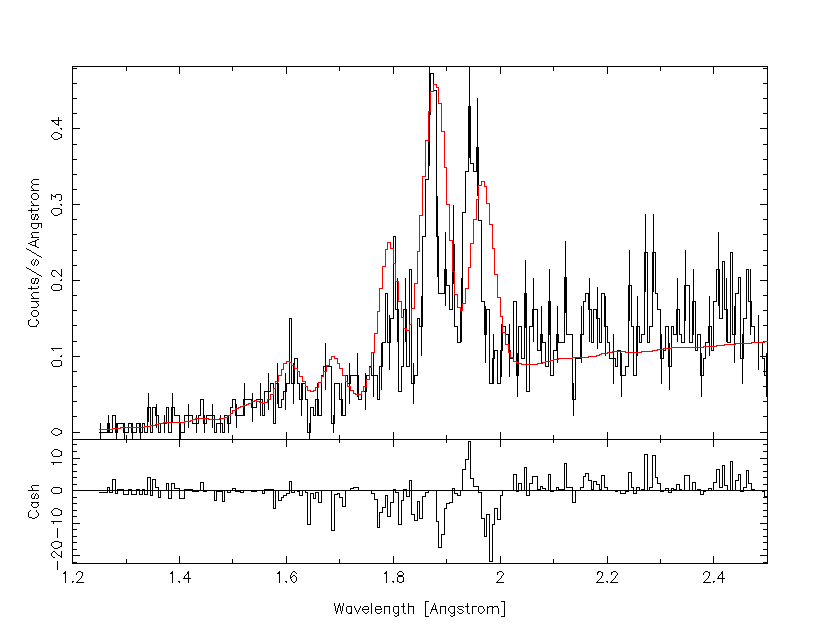
\includegraphics[width=.8\linewidth]{Chapters/Figures/aped_model_tied.png}
    \caption{The aped model with the parameters of two jets tied to each other}
    \label{fig:my_label}
\end{figure}
\newpage
\begin{figure}[h!]
    \centering
    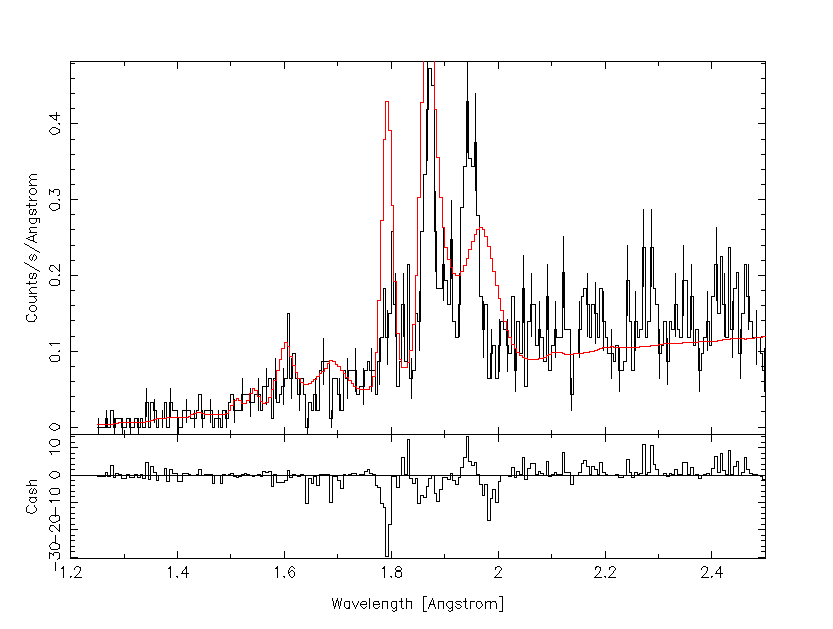
\includegraphics[width=.8\linewidth]{Chapters/Figures/aped_model_untied.png}
    \caption{The aped model with the parameters of two jets not tied to each other}
    \label{fig:my_label}
\end{figure}

10/17\\
Run the fit\_line\_gl4 script, which will produce the gaussian fits for those emission lines. The output files are named as par\_\#lines\_g4.txt. 
The first graph shows almost the same as the one created by fit plasma model script. The only difference is bin number of group\_data is 4 in the current script and is 2 in the plasma script.
Some questions about the fit\_line\_gl4 script.\\
1. Where do the values of line\-wave come from?  Why some line\_wave need to find the average?\\
Update: The line is a blend of two lines and the calculation applies the weights. For example, all lines for H-like ions would be a blend of the alpha1 and alpha2 lines\\
2. conf\_loop generates single-parameter confidence limits for specified parameters (redshift, sigma, rest\_wave.lambda, gaussian properties, etc.) Why it is generating so many files?\\
Update: for each file, it is estimating the parameters by a small regions under the gaussian curve.\\ 
3. What is the difference between the files in conf\_loop and par\_\#lines\_g4.txt?

10/18\\
More questions about fit\_line\_gl4 script.\\
1. What file should go inside load\_par("pars\_all\_lines.txt"); (line 369)? Should it be par\_9lines\_g4.txt?\\
2. How to plot a gaussian plot of just one line?\\
3. Where do those redshift values of two jets come from? Why they are different from the theoretical values? 


10/23\\
Created a new script to plot the fitted line for the spectrum. I moved the plotting command up before the confidence loop and finally got the fitted lines. However, when I changed the redshift to the one that we expect (0.0089 and 0.068), the fitted lines do not catch some important lines. 

10/30\\
To see the line at a certain wavelength is produced by which element and which jet, I plot the graph line by line

First, I plotted the continuum model without fitting any line. See Fig~\ref{fig:continuum}

\begin{figure}[h!]
    \centering
    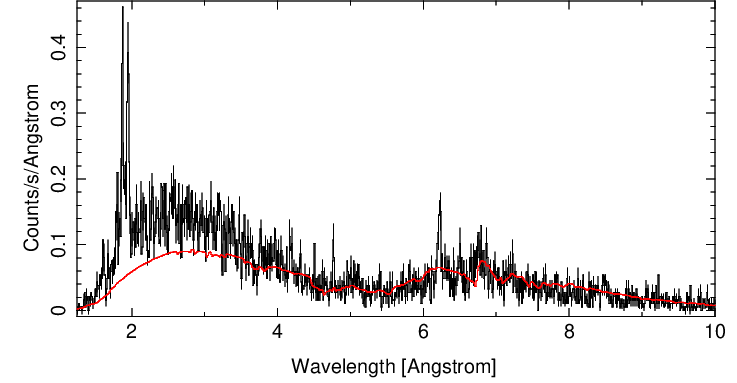
\includegraphics[width=1\linewidth]{Chapters/Figures/unfitted.png}
    \caption{The continuum model prior to fitting lines.}
    \label{fig:continuum}
\end{figure}

The final fitted graph with all lines shows in Fig~\ref{fig:all_lines_1} and Fig~\ref{fig:all_lines_2}

\begin{figure}[h!]
    \centering
    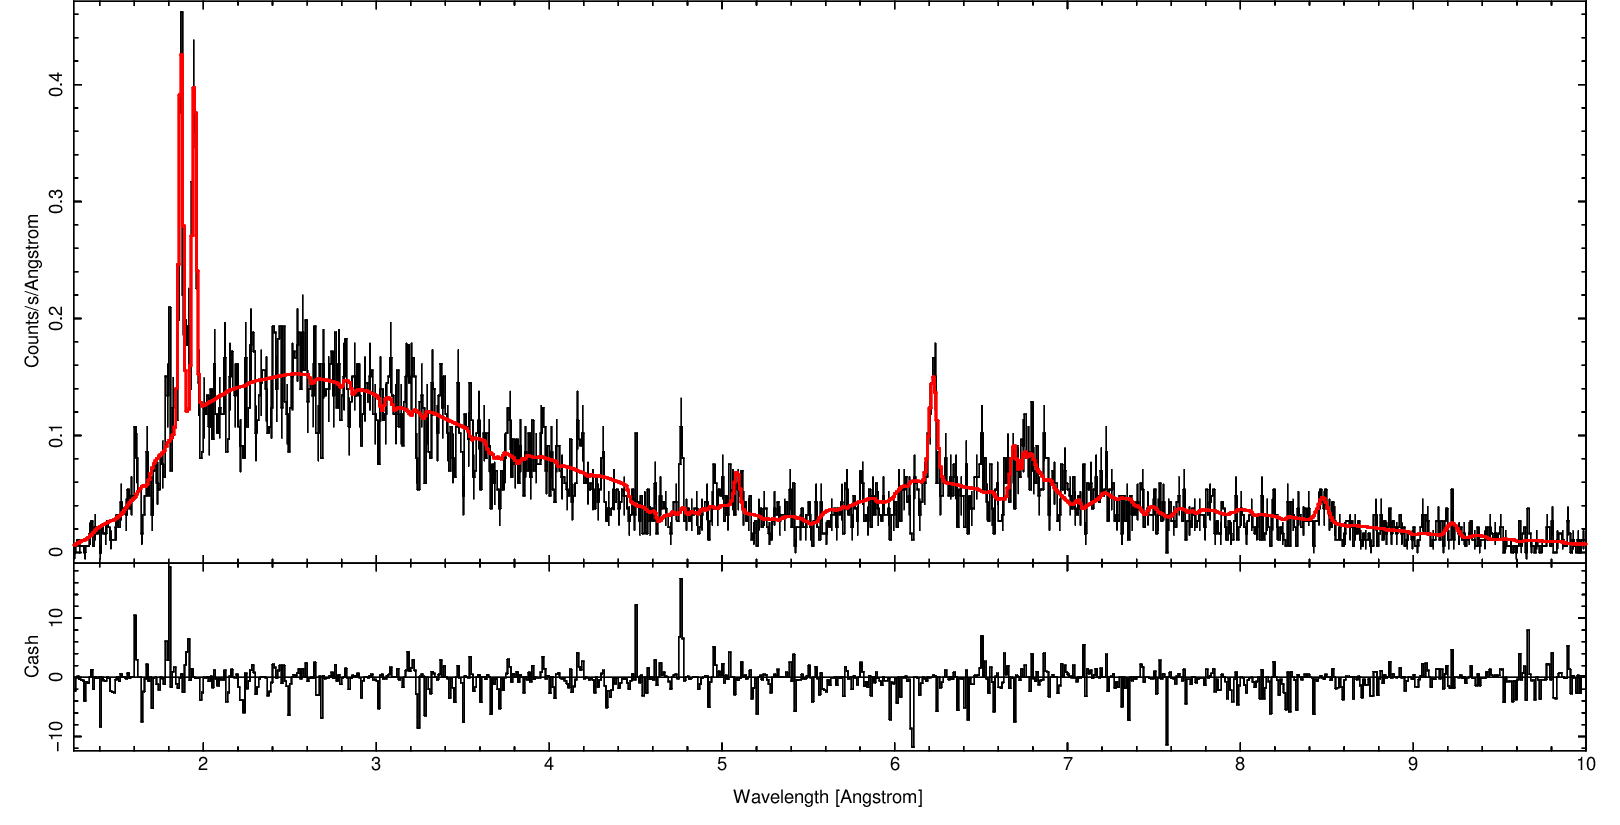
\includegraphics[width=1\linewidth]{Chapters/Figures/all_lines_fitted_heg.png}
    \caption{The fitted lines for the most prominent emissions in the HEG range}
    \label{fig:all_lines_1}
\end{figure}

\begin{figure}[h!]
    \centering
    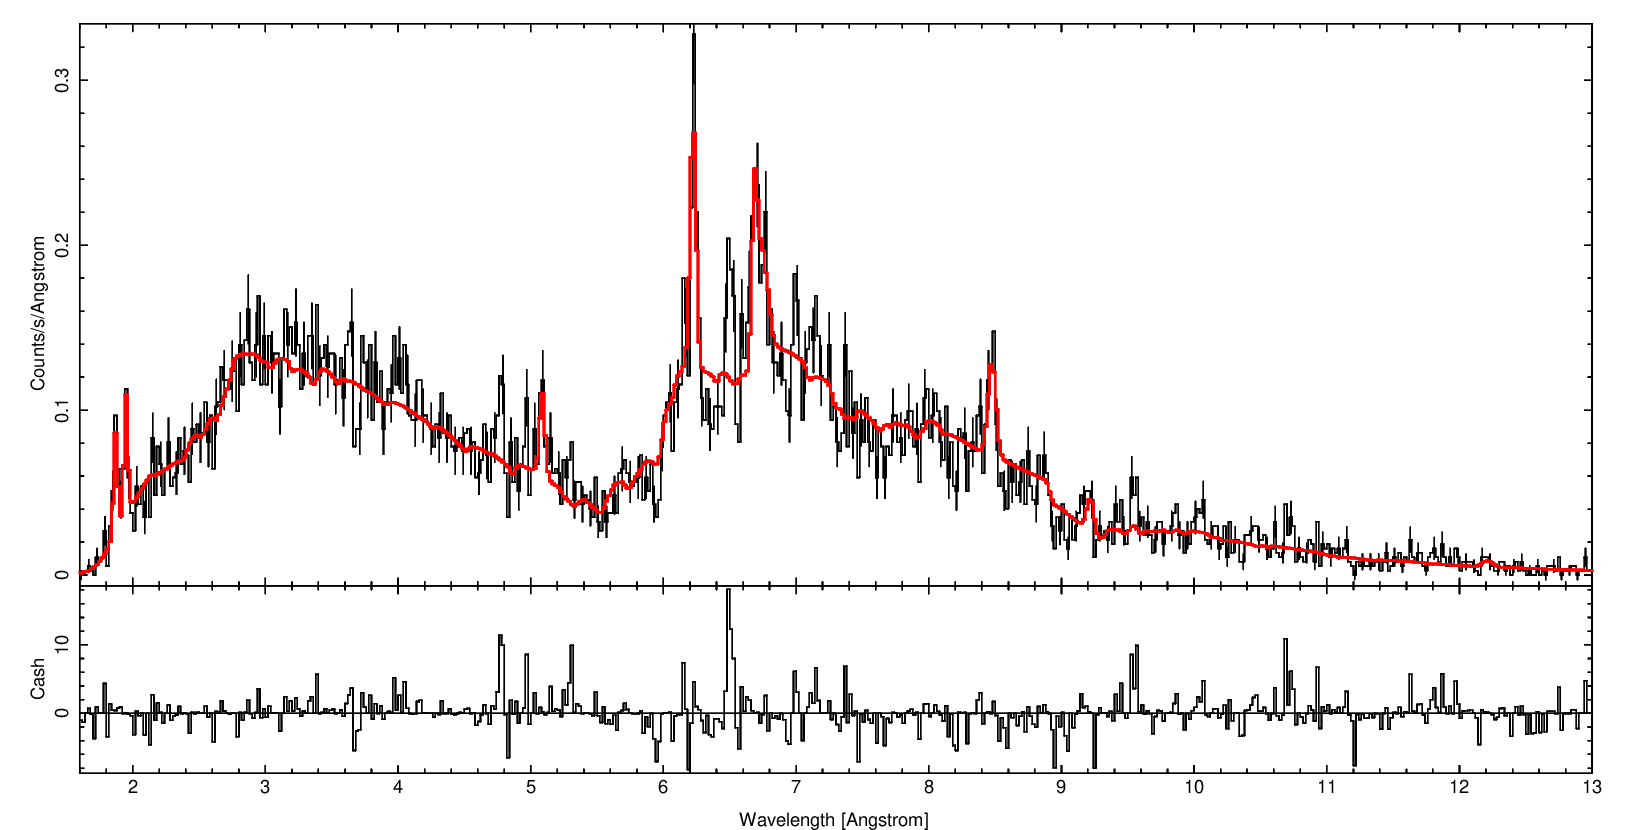
\includegraphics[width=1\linewidth]{Chapters/Figures/all_lines_fitted_meg.png}
    \caption{The fitted lines for the most prominent emissions in the MEG range}
    \label{fig:all_lines_2}
\end{figure}

Here are some zoomed-in graphs. See Fig~\ref{fig:zoomin2}, Fig~\ref{fig:zoomin1} and Fig~\ref{fig:zoomin3}

\begin{figure}[h!]
    \centering
    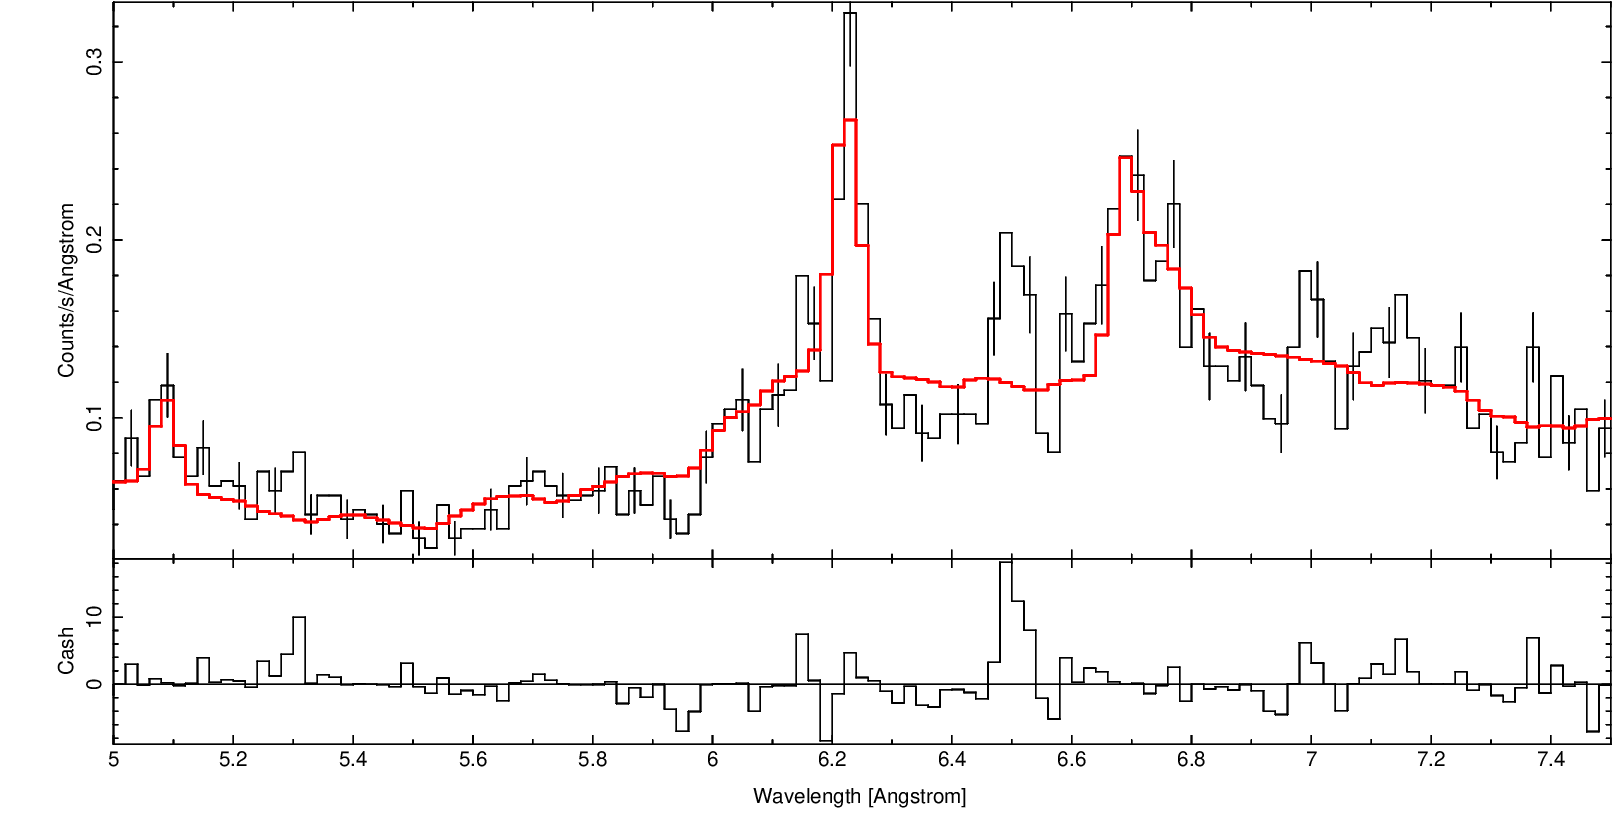
\includegraphics[width=1\linewidth]{Chapters/Figures/zoomin4.png}
    \caption{The zoom-in graph with perceived emission lines of S {\footnotesize\Romannum{15}}, Si {\footnotesize\Romannum{14}}, Si {\footnotesize\Romannum{13}r}, Si {\footnotesize\Romannum{13}i}, Si {\footnotesize\Romannum{13}f}}.
    \label{fig:zoomin2}
\end{figure}

\begin{figure}[h!]
    \centering
    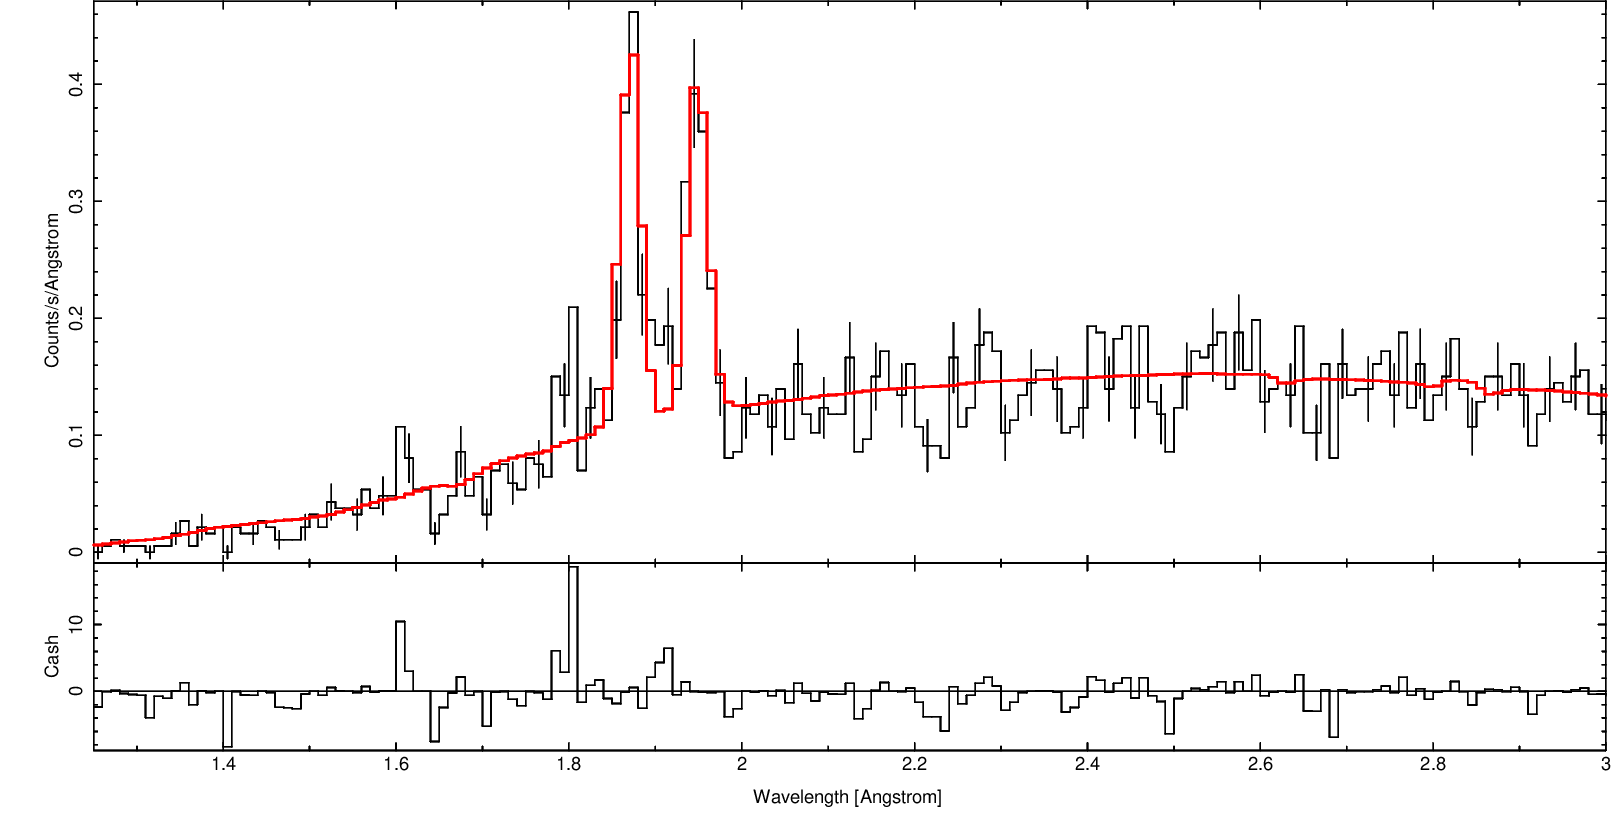
\includegraphics[width=1\linewidth]{Chapters/Figures/zoomin1.png}
    \caption{The zoom-in graph with perceived emission lines of Fe {\footnotesize\Romannum{26}}, Fe {\footnotesize\Romannum{25}}, and Fe {\footnotesize\Romannum{1}}}
    \label{fig:zoomin1}
\end{figure}


\begin{figure}[h!]
    \centering
    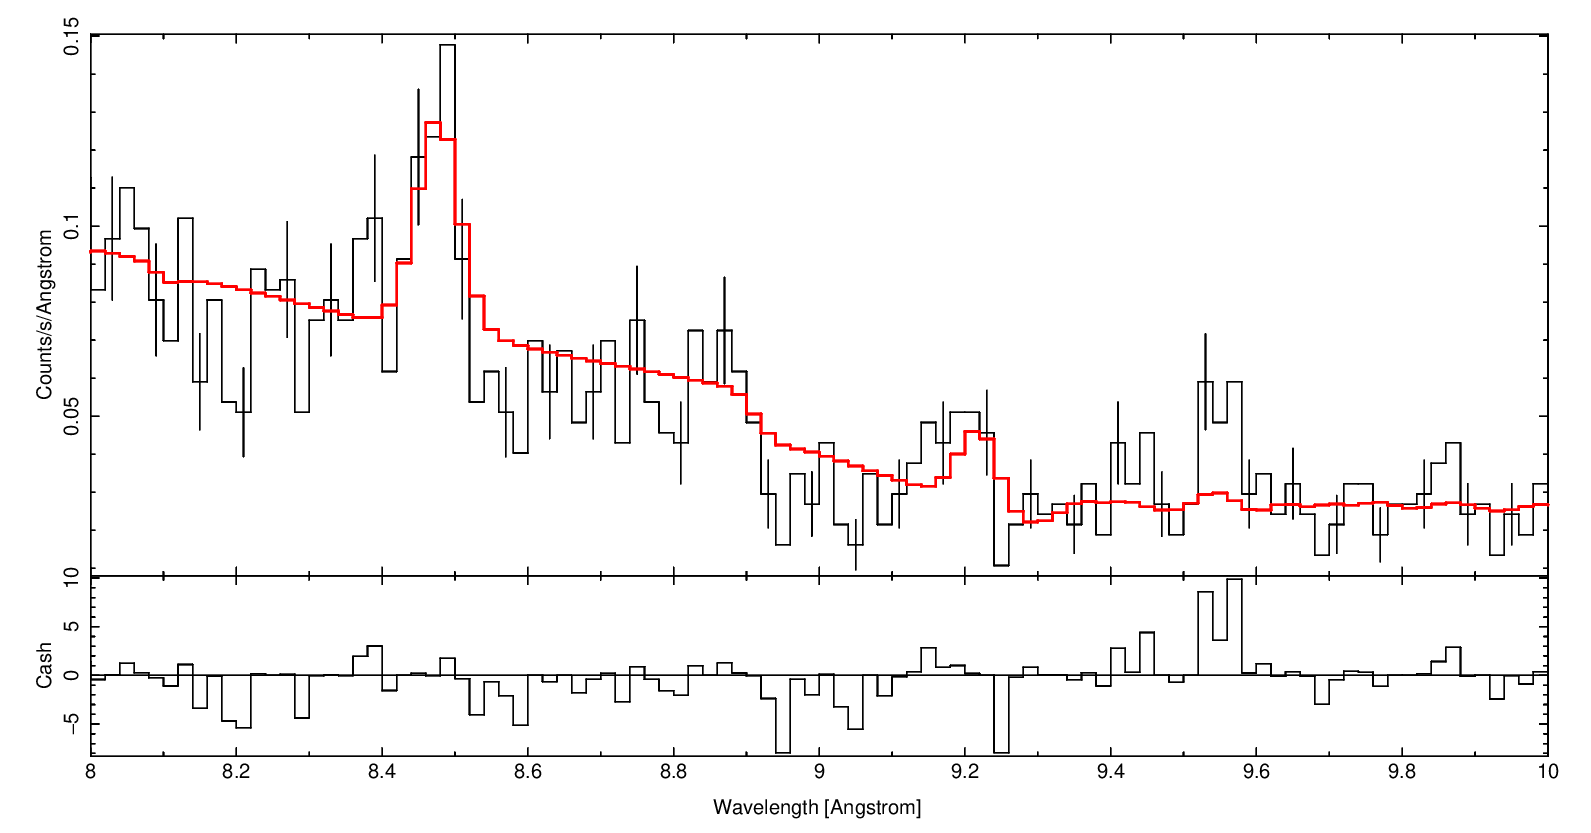
\includegraphics[width=1\linewidth]{Chapters/Figures/zoomin3.png}
    \caption{The zoom-in graph with perceived emission lines of Mg {\footnotesize\Romannum{12}}, and Mg {\footnotesize\Romannum{11}i}, Mg {\footnotesize\Romannum{11}r}, Mg {\footnotesize\Romannum{11}f}}.
    \label{fig:zoomin3}
\end{figure}

\clearpage

%\begin{verbatim}
    
\lstset{basicstyle=\footnotesize\ttfamily,breaklines=true}
\begin{lstlisting}[breaklines]
  idx  param     tie-to  freeze   value   min   max
  1  redshift(1).z    0   0  0.008250389   0.00825  0.009562  
  2  redshift(2).z    0   0   0.05083716  0.04  0.09  
  3  sigma(1).beta    0   0  0.003910095  0.0025  0.01  
  4  sigma(2).beta    0   0  0.006209743   0.005   0.015  
  5  wabs(1).nH     0   0  0.3721895     0  100000  10^22
  6  rest_wave(1).lambda  0   1     6.1823     0     0  
  7  rest_wave(2).lambda  0   1     8.4211     0     0  
  8  rest_wave(3).lambda  0   1    12.1351     0     0  
  9  rest_wave(4).lambda  0   1     5.0553     0     0  
 10  rest_wave(5).lambda  0   1    6.64795     0     0  
 11  rest_wave(6).lambda  0   1    6.68659     0     0  
 12  rest_wave(7).lambda  0   1    6.74029     0     0  
 13  rest_wave(8).lambda  0   1     1.8545     0     0  
 14  rest_wave(9).lambda  0   1     1.7799     0     0  
 15  rest_wave(10).lambda   0   1     9.1688     0     0  
 16  rest_wave(11).lambda   0   1     9.2297     0     0  
 17  rest_wave(12).lambda   0   1     9.3143     0     0  
 18  rest_wave(13).lambda   0   1     1.5883     0     0  
 19  rest_wave(14).lambda   0   1     1.8545     0     0  
 20  powerlaw(1).norm   0   0   0.01042019     0   1e+10  
 21  powerlaw(1).PhoIndex   0   0    0.93563    -2     9  
 22  gauss(1).area    0   0   0.0001349136     0     0  photons/s/cm^2
 23  gauss(1).center  0   1   6.233306     0    40  A
#=>  (1+redshift(1).z)*rest_wave(1).lambda
 24  gauss(1).sigma   0   1   0.02437282   1e-06     1  A
#=>  (1+redshift(1).z)*rest_wave(1).lambda*sigma(1).beta
 25  gauss(2).area    0   0   7.185216e-05     0     0  photons/s/cm^2
 26  gauss(2).center  0   1   8.490577     0    40  A
#=>  (1+redshift(1).z)*rest_wave(2).lambda
 27  gauss(2).sigma   0   1   0.03319897   1e-06     1  A
#=>  (1+redshift(1).z)*rest_wave(2).lambda*sigma(1).beta
 28  gauss(3).area    0   0   6.199978e-05     0     0  photons/s/cm^2
 29  gauss(3).center  0   1   12.23522     0    40  A
#=>  (1+redshift(1).z)*rest_wave(3).lambda
 30  gauss(3).sigma   0   1   0.04784087   1e-06     1  A
#=>  (1+redshift(1).z)*rest_wave(3).lambda*sigma(1).beta
 31  gauss(4).area    0   0   9.408116e-05     0     0  photons/s/cm^2
 32  gauss(4).center  0   1   5.097008     0    40  A
#=>  (1+redshift(1).z)*rest_wave(4).lambda
 33  gauss(4).sigma   0   1   0.01992979   1e-06     1  A
#=>  (1+redshift(1).z)*rest_wave(4).lambda*sigma(1).beta
 34  gauss(5).area    0   0   0.0001372658     0     0  photons/s/cm^2
 35  gauss(5).center  0   1   6.702798     0    40  A
#=>  (1+redshift(1).z)*rest_wave(5).lambda
 36  gauss(5).sigma   0   1   0.02620858   1e-06     1  A
#=>  (1+redshift(1).z)*rest_wave(5).lambda*sigma(1).beta
 37  gauss(6).area    0   0   2.145622e-05     0     0  photons/s/cm^2
 38  gauss(6).center  0   1   6.741757     0    40  A
#=>  (1+redshift(1).z)*rest_wave(6).lambda
 39  gauss(6).sigma   0   1   0.02636091   1e-06     1  A
#=>  (1+redshift(1).z)*rest_wave(6).lambda*sigma(1).beta
 40  gauss(7).area    0   0   1.301116e-05     0     0  photons/s/cm^2
 41  gauss(7).center  0   1     6.7959     0    40  A
#=>  (1+redshift(1).z)*rest_wave(7).lambda
 42  gauss(7).sigma   0   1   0.02657262   1e-06     1  A
#=>  (1+redshift(1).z)*rest_wave(7).lambda*sigma(1).beta
 43  gauss(8).area    0   0   0.0004757573     0     0  photons/s/cm^2
 44  gauss(8).center  0   1   1.948778     0    40  A
#=>  (1+redshift(2).z)*rest_wave(8).lambda
 45  gauss(8).sigma   0   1   0.01210141   1e-06     1  A
#=>  (1+redshift(2).z)*rest_wave(8).lambda*sigma(2).beta
 46  gauss(9).area    0   0   0.0004765693     0     0  photons/s/cm^2
 47  gauss(9).center  0   1   1.870385     0    40  A
#=>  (1+redshift(2).z)*rest_wave(9).lambda
 48  gauss(9).sigma   0   1   0.01161461   1e-06     1  A
#=>  (1+redshift(2).z)*rest_wave(9).lambda*sigma(2).beta
 49  gauss(10).area   0   0   6.577367e-05     0     0  photons/s/cm^2
 50  gauss(10).center   0   1   9.244446     0    40  A
#=>  (1+redshift(1).z)*rest_wave(10).lambda
 51  gauss(10).sigma  0   1   0.03614667   1e-06     1  A
#=>  (1+redshift(1).z)*rest_wave(10).lambda*sigma(1).beta
 52  gauss(11).area   0   0  -2.833654e-05     0     0  photons/s/cm^2
 53  gauss(11).center   0   1   9.305849     0    40  A
#=>  (1+redshift(1).z)*rest_wave(11).lambda
 54  gauss(11).sigma  0   1   0.03638675   1e-06     1  A
#=>  (1+redshift(1).z)*rest_wave(11).lambda*sigma(1).beta
 55  gauss(12).area   0   0   2.449444e-05     0     0  photons/s/cm^2
 56  gauss(12).center   0   1   9.391147     0    40  A
#=>  (1+redshift(1).z)*rest_wave(12).lambda
 57  gauss(12).sigma  0   1   0.03672028   1e-06     1  A
#=>  (1+redshift(1).z)*rest_wave(12).lambda*sigma(1).beta
 58  gauss(13).area   0   0   -1.86183e-05     0     0  photons/s/cm^2
 59  gauss(13).center   0   1   1.669045     0    40  A
#=>  (1+redshift(2).z)*rest_wave(13).lambda
 60  gauss(13).sigma  0   1   0.01036434   1e-06     1  A
#=>  (1+redshift(2).z)*rest_wave(13).lambda*sigma(2).beta
 61  gauss(14).area   0   0   0.0001318383     0     0  photons/s/cm^2
 62  gauss(14).center   0   1     1.8698     0    40  A
#=>  (1+redshift(1).z)*rest_wave(14).lambda
 63  gauss(14).sigma  0   1  0.007311097   1e-06     1  A
#=>  (1+redshift(1).z)*rest_wave(14).lambda*sigma(1).beta
\end{lstlisting}
%\end{verbatim}


% \begin{table}[t]
% \begin{tabular}{|p{1cm}||p{4cm}|p{2cm}|p{2cm}|p{2.5cm}|p{2cm}|p{2cm}| }
%   \hline
%   \multicolumn{7}{|c|}{Parameter Table} \\
%   \hline
%     idx & Parameter & tie-to & freeze & value & min & max\\
%     \hline
%     1 & redshift(1).z  &        0  &   0     &   0.0065721 &  -0.001094  &  0.018906  \\
%     2 & redshift(2).z    &      0   &  0    &   0.05084416  &      0.04   &     0.09\\  
%     3 & sigma(1).beta    &      0   &  0   &   0.003289482  &    0.0025    &    0.01  \\
%     4 & sigma(2).beta     &     0  &   0  &    0.005581536  &     0.005   &    0.015  \\
%     5 & wabs(1).nH     &        0  &   0   &     0.3711946  &     0     & 100000 $10^{22}$  \\
%     6 & rest\_wave(1).lambda  &  0  &   1   &     6.1823  &     0     &      0  \\
%     7 & rest\_wave(2).lambda  &  0  &   1    &    8.4211  &     0     &      0  \\
%     8 & rest\_wave(3).lambda  &  0    & 1   &     12.1351 &     0      &     0  \\
%     9 & rest\_wave(4).lambda  &  0   &  1     &   5.0553  &       0     &      0  \\
%     10 & rest\_wave(5).lambda &   0  &   1    &  6.64795  &       0     &      0  \\
%     11 & rest\_wave(6).lambda  &  0  &   1    & 6.68659  &  0    &       0  \\
%     12 &  rest\_wave(7).lambda &   0  &   1  &  6.74029  &    0      &     0  \\
%     13 &  rest\_wave(8).lambda  &  0  &   1  & 1.8545   &    0      &     0  \\
%     14 & rest\_wave(9).lambda  &  0  &   1   & 1.7799    & 0   &    0  \\
%     15 & rest\_wave(10).lambda &  0  &   1   &   9.1688    &  0  &    0  \\
%     16 & rest\_wave(11).lambda &  0  &   1   &  9.2297   &    0  &   0\\  
%     17 & rest\_wave(12).lambda &  0  &   1   &  
%     9.3143   &    0  &   0  \\
%     18 & rest\_wave(13).lambda &  0  &   1  & 1.5883   &    0  &   0  \\
%     19 & rest\_wave(14).lambda &  0  &   1  &     1.8545   &    0  &   0  \\

%   \end{tabular}
% \end{table}
\newpage
11/15
After we fit the lines, we found that there are some lines that are missed fitting. I added Fe26 with redshift 1 and S16 with redshift 1 and the fitted lines show up well. I added some labels on the line fitting graph. We found that Fe26 from the "red"/western jet is overlapping with Fe25 from the "blue"/eastern jet. Look at Fig~\ref{fig:labeled1} and Fig~\ref{fig:labeled2}
\begin{figure}[h!]
    \centering
    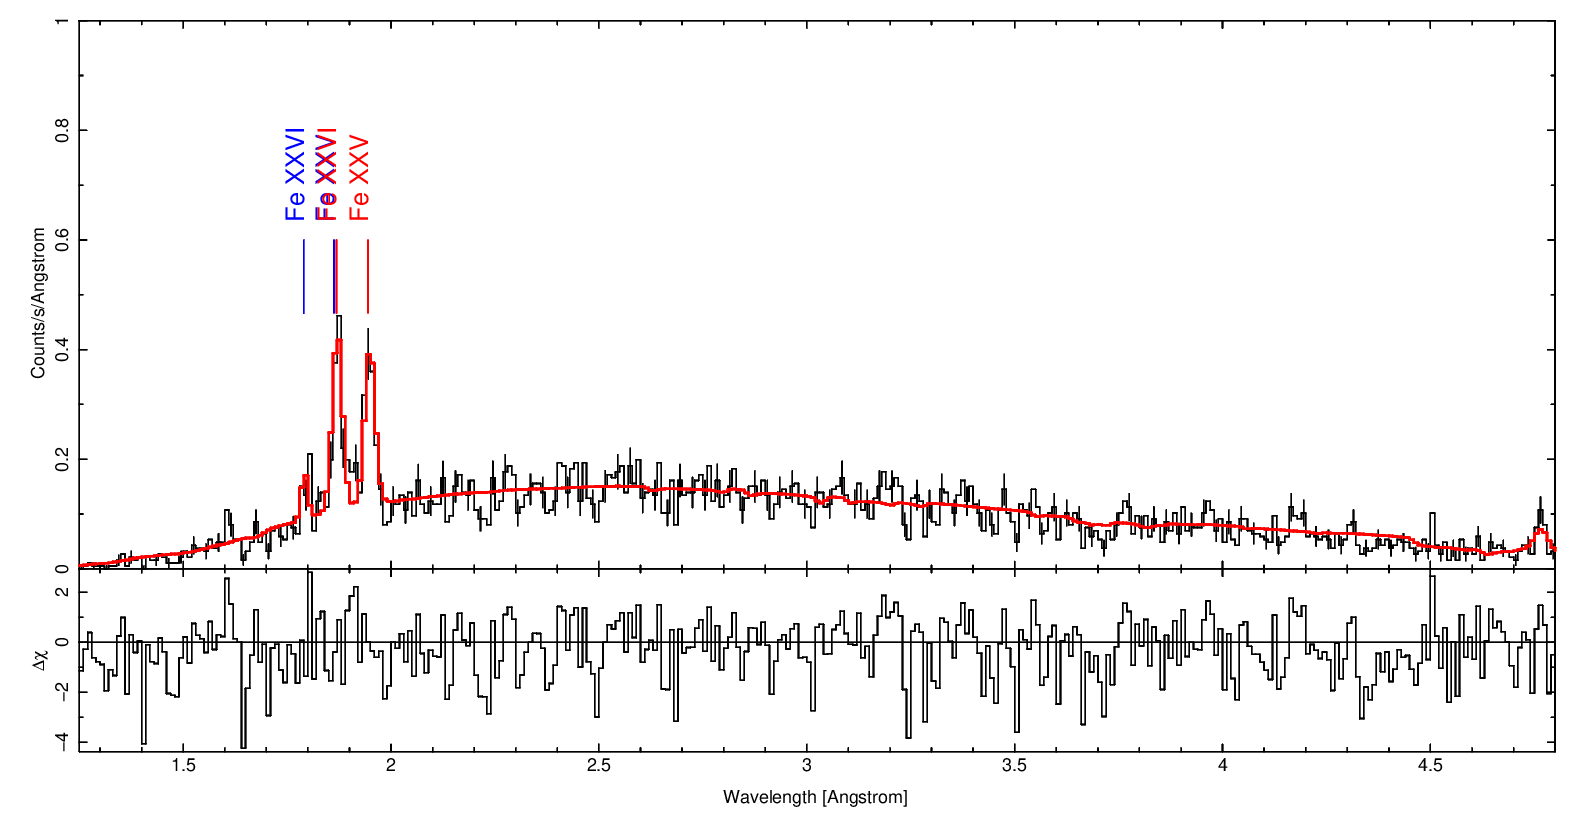
\includegraphics[width=0.9\linewidth]{Chapters/Figures/label1.png}
    \caption{The HEG spectrum of emission lines with labeled elements}.
    \label{fig:labeled1}
\end{figure}

\begin{figure}[h!]
    \centering
    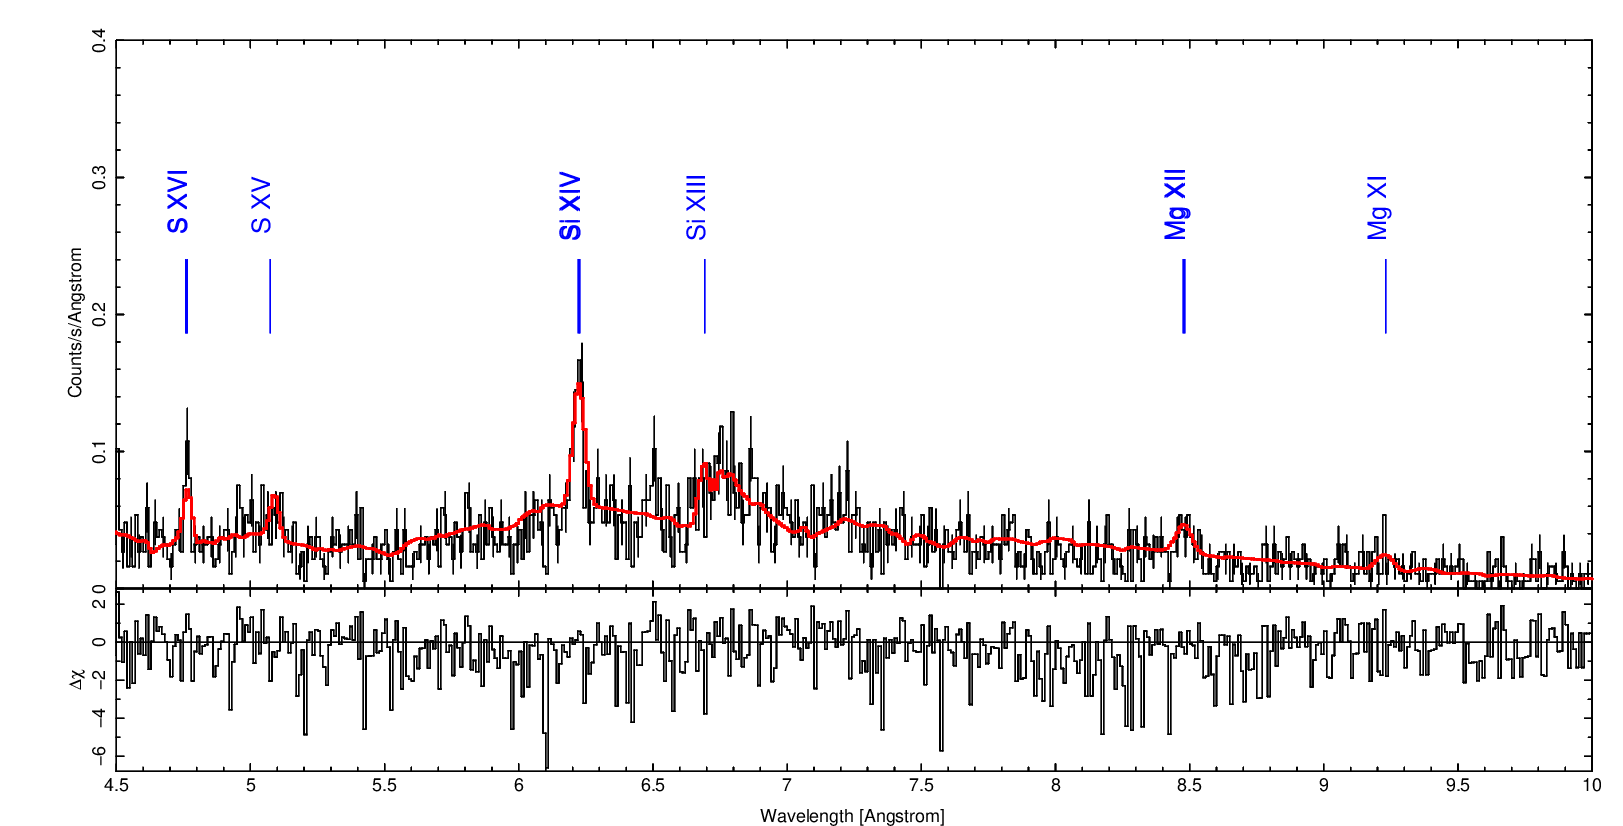
\includegraphics[width=0.9\linewidth]{Chapters/Figures/label2.png}
    \caption{The HEG spectrum of emission lines with labeled elements}.
    \label{fig:labeled2}
\end{figure}

\newpage
11/21\\
I ran the conf\_loop command for lines fit. The file that created by it is called pars\_allsave, which contains the confidence interval for all the parameters.\\
Questions to ask Herman:\\
In the code :
\begin{lstlisting}
load_par("par_9lines_g4.txt");
wline = [23,26,29,32,35,38,47,50,59,62];
nline = length(wline);
for(i=0;i<nline;i++) {
   idx = wline[i];
   gpi = get_par_info( idx );
   variable val=gpi.value;
   set_par(idx, val, 0, 0.3*val, 3.0*val);
}
\end{lstlisting}
Why we free those parameters that are for the Gaussian centers?

I loaded this save\_par file in the fit line script and look at the output plot and compare it with the previous one.\\
There is no big difference between two plots and I will check the plot with the parameter file and see where are those negative areas.\\

11/27
The three elements that have the negative area are restwave(11)[Mg11i], restwave(13)[Ni1], and restwave(14)[Fe25], which have line center at 9.292653 A, 1.669105 A, and 1.867149 A. By looking at the graph, I found the line center values in the parameter file does not exactly match the peak of the gaussian, which corresponds to a gap prior or after the peak.\\
I will free the line centers. Nothing changes.

Then I changed the values in the parameter file for the plasma model corresponding to the values that are found by the lines fit. And I start the cash fit and the conf loop.

11/28\\
The plasma fit finished. The fitting does not work well at the peak at about 1.95 and 1.5 - 1.8 range. 
Questions:\\
1. When the second jet is not tied to the first jet, how should we change the limit?\\
2. What parameters should we tie? 



11/29\\
Try to tweak the plasma model\\ 
How to set the range of the plasma model??\\

Jet with more emission lines (the jet with redshift ~ 0.0065 in our case) has smaller turbulence because the lines are narrower.\\

When I make the range of norms large, the width of the gaussian becomes large. 
When I manually increase the turbulence of jets the height of the peaks decrease. 
For the first jet, norm4 largely decides the height of the peak while norm1, 2, and 3 need to be increased a lot to see the change. 

 Look at Fig~\ref{fig:labeled1} and Fig~\ref{fig:labeled2}
 
 \newpage
\begin{figure}[h!]
    \centering
    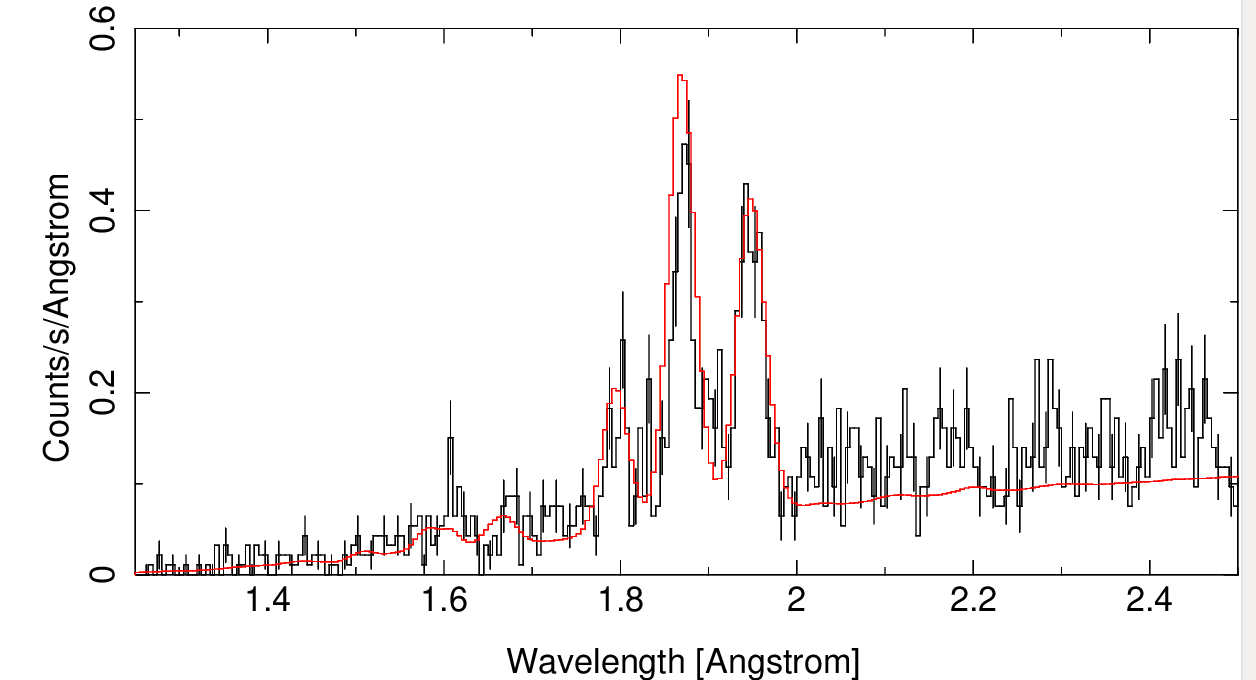
\includegraphics[width=0.9\linewidth]{Chapters/Figures/short_wavelength.png}
    \caption{The plasma fitting model for the longer wavelength range with manually twisted parameters}.
    \label{fig:manual_long}
\end{figure}

\begin{figure}[h!]
    \centering
    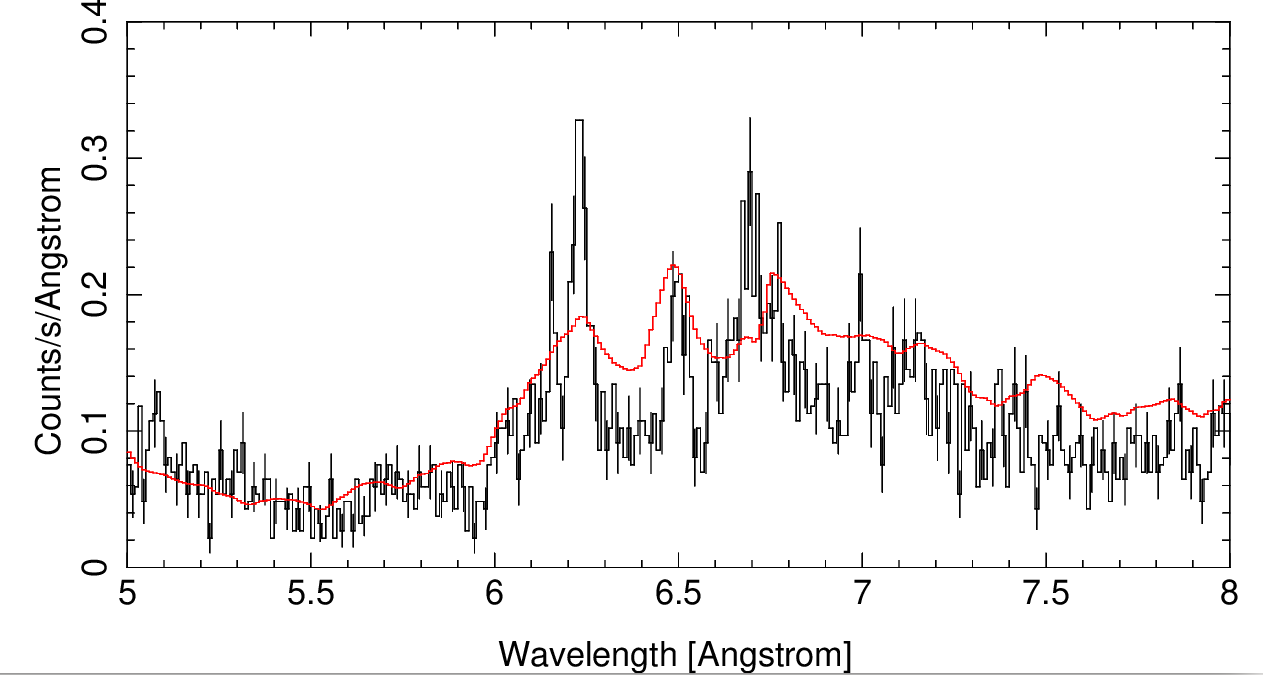
\includegraphics[width=0.9\linewidth]{Chapters/Figures/long_wavelength.png}
    \caption{The plasma fitting model for the shorter wavelength range with manually twisted parameters}.
    \label{fig:manual_short}
\end{figure}


12/3\\
Adding more lines in the line fit graph as Herman suggested in the latest email.\\
How to solve the problem of "continuum is too high, due (probably) to unmodeled lines"?\\

I tuned the parameters for plasma model and got better graphs.\\
Some notes:\\
1. norm1 for jet1 controls peak at 6.5-7 A.\\

12/11\\
I downloaded the longer observation 20131 from \url{https://cda.harvard.edu/chaser/mainEntry.do}

1/5\\
To create pha and mfa files, setup\_obsdir is needed to run. However, I cannot run setup\_obsdir {dir of observation} directly. Instead, I need to find where it is and run bash {dir of setup\_obsdir} observation. Might need to define sth. in .bashrc. \\
All files are created.\\



2/3\\
Use the head command to look at the event file in different parts of the long observation.\par

Mission Elapsed Time (MET) is used by NASA during their space missions, most notably during their Space Shuttle missions. Because so much of the mission depends on the time of launch, all events after launch are scheduled on the Mission Elapsed Time. This avoids constant rescheduling of events in case the launchtime slips. The MET-clock is set to zero at the moment of liftoff and counts forward in normal days, hours, minutes, and seconds.\\
MJD\_OBS =  5.8343629734065E+04 / Modified Julian date of observation \par
Found the Tstart and Tend in the evt0 file and calculated the time intervals of the four parts. Entered the time in XMM\/Chandra seconds since 1998.0 TT (decimal) on website \url{https://go.nasa.gov/2UIGMjk} to find the MJD.

\begin{table}[t]
\caption{The observation information for different parts of the long observation and expected red shifts}
\centering 
% used for centering table
\begin{tabular}{c c c c c}
\hline
\hline                       
Part & Starting Time & Ending Time & zred & zblue\\ [0.5ex]
\hline
0 & 58343.62893332 & 58343.85713227 & -0.009697 & 0.086842\\
1 & 58343.85713227 & 58344.08533122& -0.010609 & 0.087753\\
2 & 58344.08533122 & 58344.31353015 & -0.011065 & 0.0881213 \\
3 & 58344.31353015 & 58344.54172910 & -0.01105 & 0.088195\\
4 &  &  & -0.010572 & 0.087716\\
[1ex]
\hline
\end{tabular}
\label{table:nonlin}
\end{table}\par


2/5\\
Then I used the similar method that I did in the short observation to find the theoretical red-shifted and blue-shift wavelengths for 5 parts. Need to make a table for the rest wavelengths, observed wavelengths, and line flux.
2/9\\
I fit the lines for 5 parts and found that the red shift for the red jet is much larger than the theoretical one.\\

\begin{table}[t]
\caption{SS 433 Western Jet (smaller red shift) Lines}
\centering 
% used for centering table
\begin{tabular}{c c c  }
\hline
\hline                       
$\lambda_{rest}$ (\AA)& $\lambda_{obs}$ (\AA) & Flux ($10^{-6}$ photons cm$^{-2}$s$^{-1}$)\\ [0.5ex]
\hline
\multirow{7}{4em}{6.1823} & 6.406382 & 0.0001953477\\
 & 8.726329 & 8.070485e-05\\
\multirow{7}{4em}{6.64795} & 6.88891 & 0.0001081967\\
\multirow{7}{4em}{6.68659} & 6.928951 & 1.038041e-05\\
\multirow{7}{4em}{6.74029} & 6.984597 & 1.630129e-05\\
\multirow{7}{4em}{5.0553} & 5.238533 & 9.152973e-05\\
\multirow{7}{4em}{1.592} & 1.649703 & 0.0002589697\\
\multirow{7}{4em}{1.8545} & 1.921718 & 0.001026132\\
\multirow{7}{4em}{1.7799} & 1.844414 & 0.0002451663\\
\multirow{7}{4em}{9.1688} & 9.50113 & 3.047942e-05\\
\multirow{7}{4em}{9.2297} & 9.564238 & 1.607879e-06\\
\multirow{7}{4em}{9.3143} & 9.651904 & 4.382468e-05\\
\multirow{7}{4em}{4.73} & 4.901442 & 0.0001567437\\
\multirow{7}{4em}{6.64795} & 7.185847 & 3.4199e-05\\
\multirow{7}{4em}{6.68659} & 7.227614 & -6.881935e-05\\
\multirow{7}{4em}{6.74029} & 7.285659 & 5.898873e-05\\
\multirow{7}{4em}{6.1823} & 6.682521 & 7.490763e-05\\
 & 6.400339 & 0.0002093213\\
 & 8.718098 & 9.722996e-05\\
 & 6.882412 & 9.122088e-05\\
 & 6.922415 & 1.795798e-05\\
 & 6.978009 & 4.944435e-05\\
\multirow{7}{4em}{8.4211}& 5.233592 & 9.761647e-05\\
 & 1.648147 & 0.0002369767\\
 & 1.919905 & 0.0008224793\\
 & 1.842674 & 0.0002559987\\
 & 9.492168 & 3.505377e-05\\
 & 9.555216 & -2.071569e-05\\
 & 9.642799 & 2.584576e-05\\
 & 4.896819 & 0.0001333559\\
 & 7.189345 & -6.182377e-07\\
 & 7.231132 & -4.983215e-05\\
 & 7.289205 & 4.465996e-05\\
 & 6.685774 & 7.39148e-05\\
 & 6.400427 & 0.0001816885\\
 & 8.718218 & 7.379159e-05\\
 & 6.882506 & 8.407732e-05\\
 & 6.92251 & 1.787087e-05\\
 & 6.978104 & 4.133396e-05\\
 & 5.233664 & 9.000698e-05\\
 & 1.64817 & 0.0002635255\\
 & 1.919931 & 0.0007689837\\
 & 1.842699 & 0.0002975289\\
 & 9.492298 & 6.446505e-06\\
 & 9.555347 & 1.417067e-05\\
 & 9.642932 & -3.449051e-06\\
 & 4.896886 & 0.0001191925\\
 & 7.189102 & -3.62957e-05\\
 & 7.230887 & 1.030425e-05\\
 & 7.288959 & 2.429657e-05\\
 & 6.685547 & 4.134544e-05\\
 & 6.400808 & 0.0002132997\\
 & 8.718736 & 5.533479e-05\\
 & 6.882916 & 7.374446e-05\\
 & 6.922921 & 2.188877e-05\\
 & 6.978519 & 5.132219e-05\\
 & 5.233975 & 6.269798e-05\\
 & 1.648268 & 0.0002554855\\
 & 1.920046 & 0.0008173814\\
 & 1.842809 & 0.0002206411\\
 & 9.492863 & 5.745678e-05\\
 & 9.555915 & -2.604159e-05\\
 & 9.643505 & 4.019557e-05\\
 & 4.897177 & 0.0001415489\\
 & 7.202428 & 4.392368e-05\\
 & 7.244291 & -0.0001021545\\
 & 7.30247 & 0.0001004292\\
 & 6.69794 & 7.134898e-05\\
 & 6.396571 & 0.0002129926\\
 & 8.712965 & 7.42718e-05\\
 & 6.87836 & 8.21608e-05\\
 & 6.918339 & 1.370373e-05\\
 & 6.9739 & 5.211237e-05\\
 & 5.230511 & 0.0001347571\\
 & 1.647177 & 0.0001451571\\
 & 1.918775 & 0.0008333993\\
 & 1.841589 & 0.0003086422\\
 & 9.48658 & 7.023839e-05\\
 & 9.54959 & -5.605822e-05\\
 & 9.637123 & 4.592911e-05\\
 & 4.893936 & 0.0001474191\\
 & 7.218701 & 4.583201e-07\\
 & 7.260659 & -8.00107e-05\\
 & 7.318969 & 9.137724e-05\\
 & 6.713073 & 5.978347e-05\\
[1ex]
\hline
\end{tabular}
\label{table:nonlin}
\end{table}\par



\begin{figure}[h!]
    \centering
    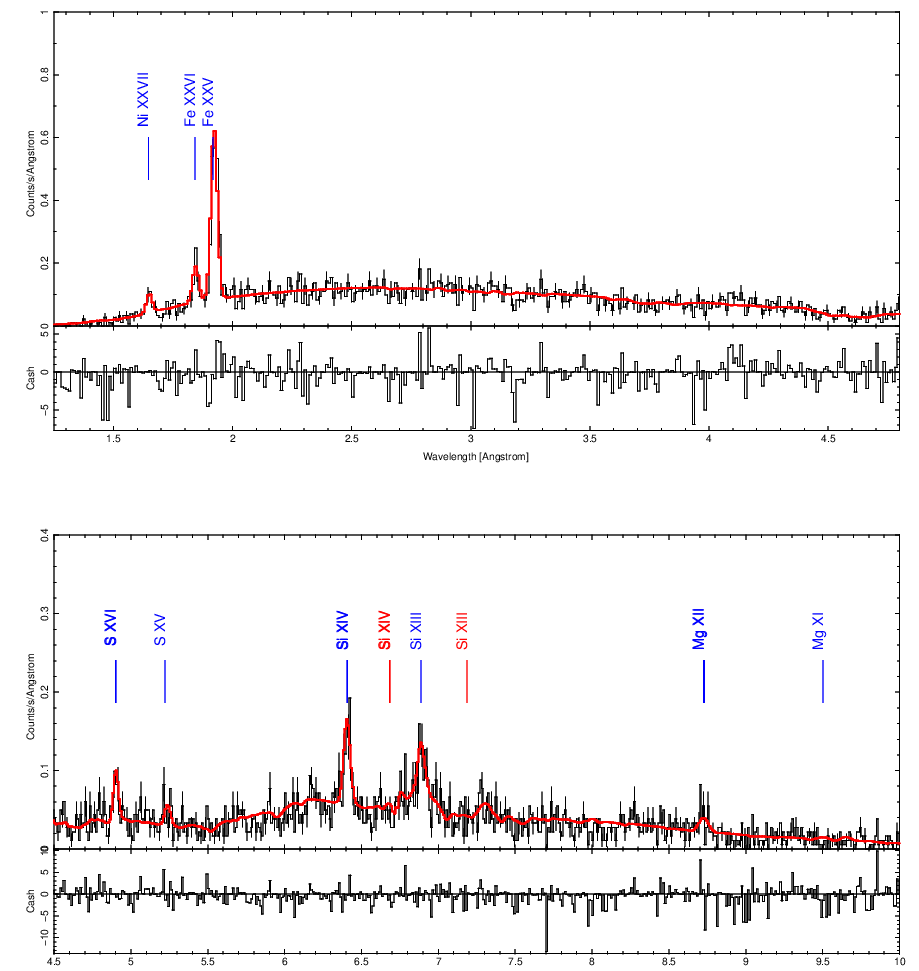
\includegraphics[width=\linewidth]{Chapters/Figures/part0_heg.png}
    \caption{The line fit graph for the HEG spectrum of part 0 of the long observation}
    \label{fig:part0}
\end{figure}

\begin{figure}[h!]
    \centering
    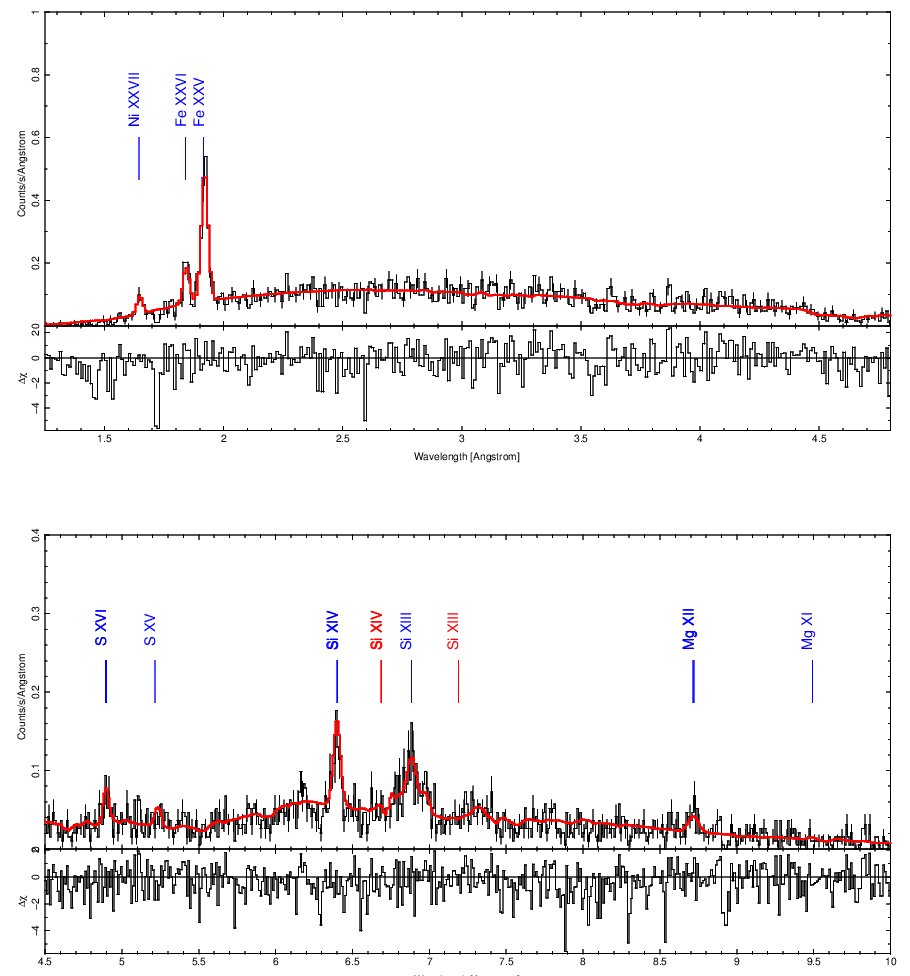
\includegraphics[width=\linewidth]{Chapters/Figures/part1_heg.png}
    \caption{The line fit graph for the HEG spectrum of part 1 of the long observation}
    \label{fig:part1}
\end{figure}

\begin{figure}[h!]
    \centering
    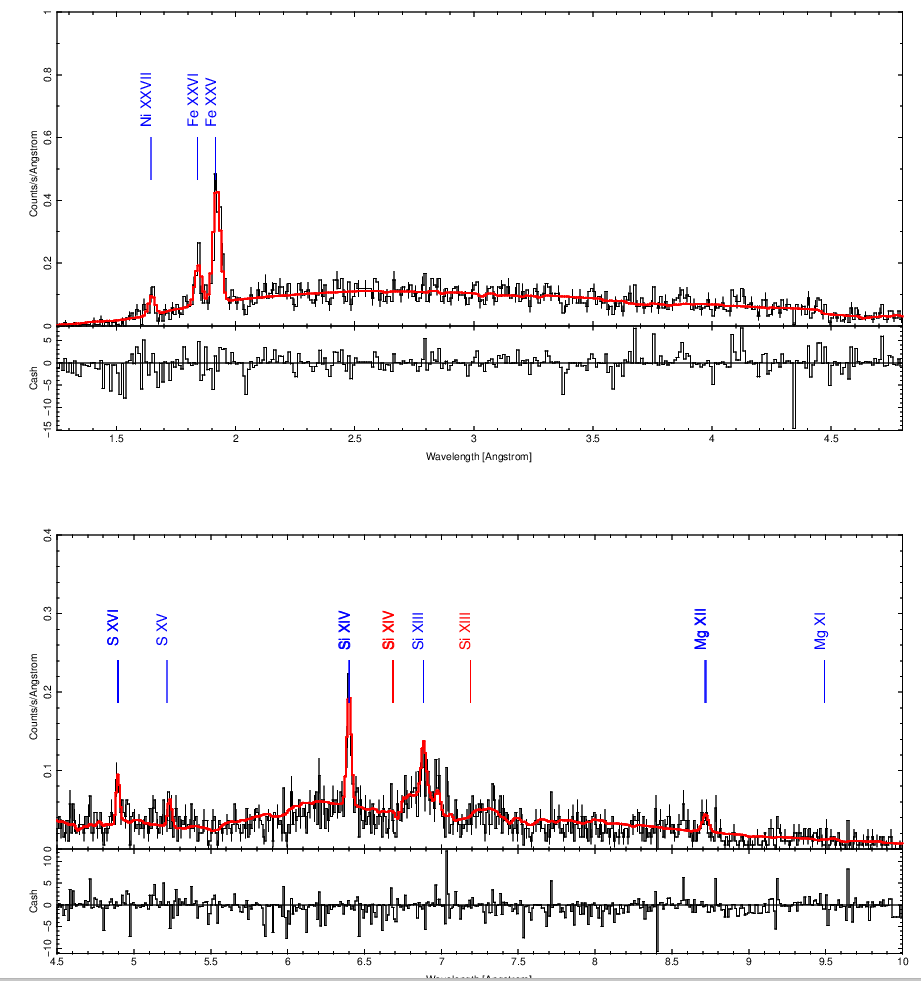
\includegraphics[width=\linewidth]{Chapters/Figures/part2_heg.png}
    \caption{The line fit graph for the HEG spectrum of part 2 of the long observation}
    \label{fig:part2}
\end{figure}

\begin{figure}[h!]
    \centering
    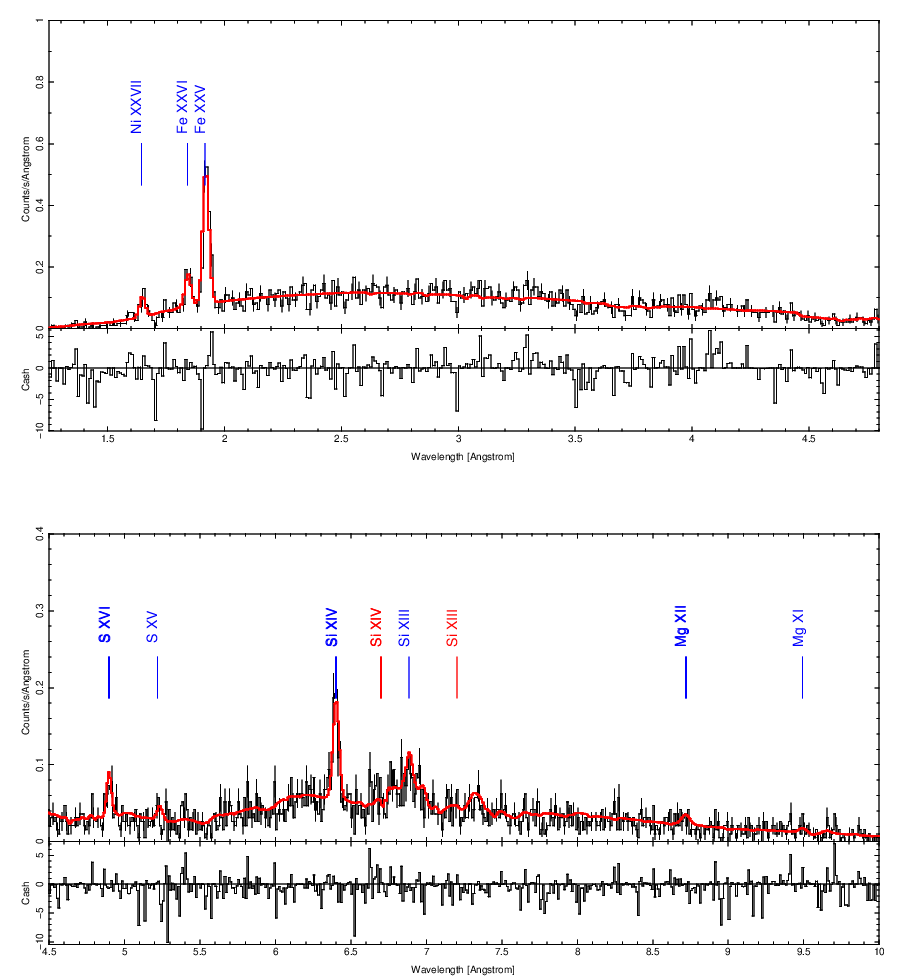
\includegraphics[width=\linewidth]{Chapters/Figures/part3_heg.png}
    \caption{The line fit graph for the HEG spectrum of part 3 of the long observation}
    \label{fig:part3}
\end{figure}

\begin{figure}[h!]
    \centering
    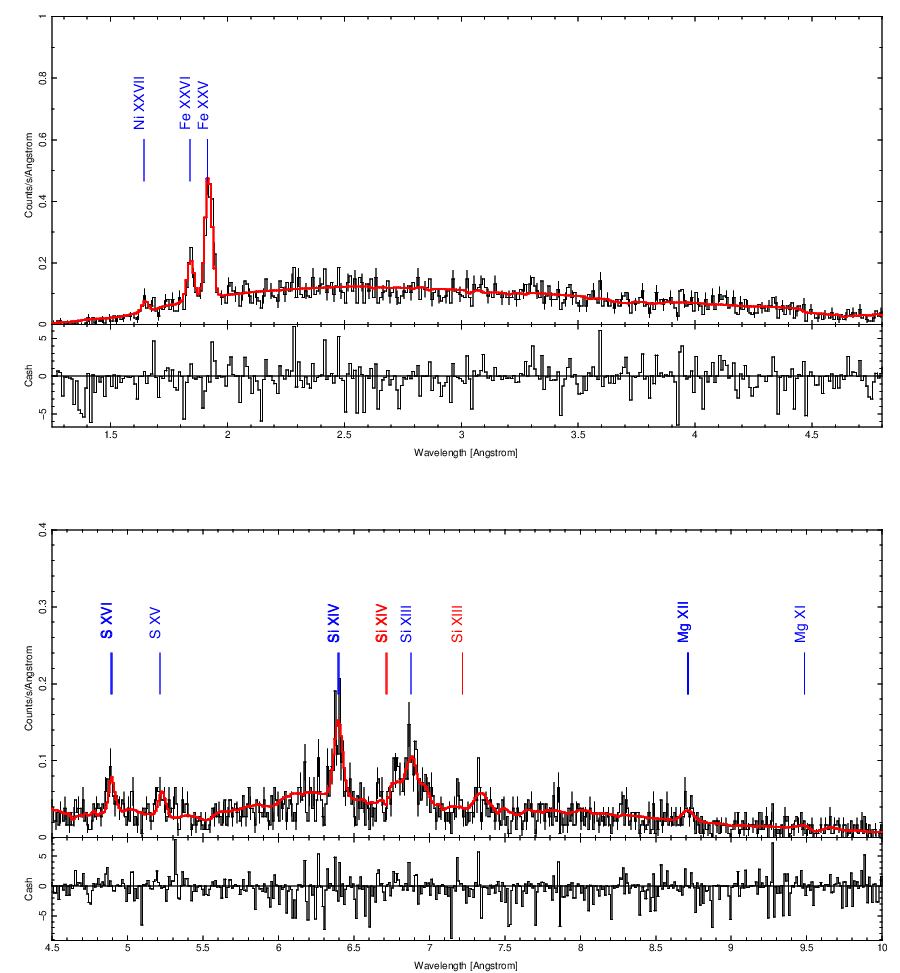
\includegraphics[width=\linewidth]{Chapters/Figures/part4_heg.png}
    \caption{The line fit graph for the HEG spectrum of part 4 of the long observation}
    \label{fig:part4}
\end{figure}



3/2\\
I am making the following graphs:\par
1. Observed redshift changes during 5 periods of the long observation comparing to the theoretical values; the redshifts from the short observation is also plotted.\par
2. Observed flux changes of emission lines from both jets (two plots) over time. Compare the flux change of these lines with the corresponding ones in the short observation.\par

One thing needs to be aware of is that Fe26 (from blue jet) and Fe25 (from red jet) overlap in the short observation. Since Fe25 (from the red jet) is fit first, the flux is significant. And thus the flux of Fe26 (from the blue jet) is small, even becomes negative. Therefore, I plot the flux as 0 for Fe26\par

For the long observation, there is only a few lines are from the blue jet. View Si13rif as a whole thing, is it ok?

3/3\\
For Fe 25 in the red jet, since its value is uncertain in the short observation, its fitted value is a negative number with large errors. I plotted it as 0 in the short observation.\par
Is it possible that we mix up the two jets?\par

3/24\\
I made the plot of the power-law spectra over the long observation. Instead of the fact that the normalization of the spectra increase due to accretor coming out of the eclipse, the normalization actually decreases over 5 parts. The spectra slope (photon index) first increases and then decreases. \par
Now I am going to use another method to test the redshift values. Put a gaussian at places where I think there should be a line and let ISIS to fit, then check what would be the wavelength.





\clearpage{}
\section{Some Linux command}
\# compile and run c files including math library\\
\textbf{gcc filename.c -lm}\\
\# extract .tar file\\
\textbf{tar -xvf}\\
\# extact tar.gz file\\
\textbf{tar -xzf *.tar.gz}\\
\# extract .gz file\\
\textbf{gunzip *.gz}\\
\# .bashrc is a shell script that Bash runs whenever it is started interactively. It initializes an interactive shell session. You can put any command in that file that you could type at the command prompt.\\
\textbf{gedit .bashrc}\\
\# Look at a pdf file\\
\textbf{xdg-open filename.xxx}
\# Transpose a file
\textbf{datamash --no-strict transpose < table.txt}\\




  % \documentclass[12pt]{article}
% \usepackage[utf8]{inputenc}	% Para caracteres en español
% \usepackage{amsmath,amsthm,amsfonts,amssymb,amscd}
% \usepackage{multirow,booktabs}
% \usepackage[table]{xcolor}
% \usepackage{fullpage}
% \usepackage{lastpage}
% \usepackage{enumitem}
% \usepackage{fancyhdr}
% \usepackage{mathrsfs}
% \usepackage{ textcomp }
% \usepackage{ gensymb }

% \usepackage{wrapfig}
% \usepackage{setspace}
% \usepackage{indentfirst}
% \usepackage{calc}
% \usepackage{multicol}
% \usepackage{cancel}
% \usepackage[retainorgcmds]{IEEEtrantools}
% \usepackage[margin=3cm]{geometry}
% \usepackage{amsmath}
% \usepackage{siunitx}
% \usepackage[final]{pdfpages}

% \newlength{\tabcont}
% \setlength{\parindent}{0.0in}
% \setlength{\parskip}{0.05in}
% \usepackage{empheq}
% \usepackage{framed}
% \usepackage[most]{tcolorbox}
% \usepackage{xcolor}


% \usepackage[round]{natbib}
% \bibliographystyle{plainnat}
% \colorlet{shadecolor}{orange!15}
% \parindent 0in
% \parskip 12pt
% \geometry{margin=1in, headsep=0.25in}
% \theoremstyle{definition}
% \newtheorem{defn}{Definition}
% \newtheorem{reg}{Rule}
% \newtheorem{exer}{Exercise}
% \newtheorem{note}{Note}
% \newcommand{\norm}[1]{\left\lVert#1\right\rVert}
% \doublespacing

% \newcommand{\dtoprule}{\specialrule{1pt}{0pt}{0.4pt}\specialrule{0.3pt}{0pt}{\belowrulesep}}
% \newcommand{\dbottomrule}{\specialrule{0.3pt}{0pt}{0.4pt}\specialrule{1pt}{0pt}{\belowrulesep}}
% \newcommand{\rncaps}[1]
%     {\MakeUppercase{\rncaps #1}}

\chapter{Introduction to X-ray Binary Systems and SS 433}
\section{The General Introduction and the Layout}
Understanding the physical conditions and evolution of relativistic jets from compact objects of an X-ray binary system is a challenge. SS 433 is the only source so far detected that has a pair of persistently precessing jets. Furthermore, it is the only jet source that shows spectral lines from many different elements \citep{Margon1980}. Therefore, the micro-quasar SS 433 offers an unique laboratory to probe its jet’s physical conditions. While previous radio and optical observations have given important information about the jet's motion and radiative properties, both the radio and the optical emission originates farther away than the X-ray does. Since X-ray emissions probe the most inner regions of the system (from distances \textless $4\times 10^{14}$ cm down to $\sim 10^{12}$ cm or less from the compact object \citep{Marshall2013}), they stand out to answer the fundamental questions about high energy astrophysics. What is the physical mechanism that launches the jet? How temperature and ionization state change along the jet?\par 

The project presented in this thesis is analyzing the Chandra/HETGS spectra of SS 433 getting from a 116 sec observation during August 10-14, 2018. The whole observation is split into a 20 ksec short observation 3 days before an eclipse that happened on August 10, 2018 and a 96 ksec long observation from the middle to the end of the eclipse beginning on August 13, 2018. Two phenomenological models were used to fit to the spectra from both short and long observations, which provide the redshift values and fluxes of the emission lines. A four-temperature plasma model was also fit to the data, studying the physical properties of the jet. The focus is on comparing the properties of emission lines between the short and the long observations and studying the evolution of the spectra within the long observations.





\section{X-ray binaries}
\subsection{Introduction to X-ray binaries}
An X-ray binary system consists of a compact object, which can be a black hole or a neutron star, gravitationally bounded to another star. The formation of an X-ray binary system is as follows: The more massive star in a binary will evolve more rapidly and explode as a supernova, leaving either a black hole or a neutron star. X-rays are generated in binary systems because of accretion of matter, coming from the optical companion, onto the compact objects. Therefore, the compact object is often called the accretor and the companion star is called the donor. \par 

X-ray binary systems can be divided in two different sub-classes. One of the sub-classes is the High Mass X-ray Binaries (HMXBs), where the donor is significantly more massive than the Sun. The other sub-class is the Low Mass X-ray Binaries (LMXBs) where the donor is a late - type star, with $M \leq M_\odot$. 

\subsection{Accretion Processes in X-ray Binaries}
There are two ways for the compact object to accrete material from the companion star. The first case is when either the size of the donor expands due to the nuclear fusion, or the binary separation shrinks due to the loss of angular momentum caused by gravitational radiation or magnetic braking. The Roche lobe is the region of a star within which the orbiting material is gravitationally bound to that star. The donor then fills its Roche lobe at some point and the matter flows from the donor toward the accretor through the inner Lagrangian point $L_1$ (See Figure~\ref{roche}). The inflowing material forms an accretion disc around the accretor due to the conservation of angular momentum. This process is called \textbf{Roche lobe overflow}. The second case is when the donor is a hot star contained within its Roche lobe but ejects some of its mass in the form of a stellar wind. Some of this wind is captured gravitationally by the accretor. This process is called \textbf{stellar wind accretion}.\par


The strong gravitational field of a compact object accelerates the accreting material from the donor. In the case of Roche lobe overflow, the matter that is transferred from the donor to the accretor does not land on the accretor immediately. Since the particles in the accreted material experience collisions with each other, frictional heating radiates energy away, reducing the particles' angular momentum. It allows the particle to drift inwards, driving the inward spiral. ion mechanism depends on the equipotential surfaces of inary system. The equipotential surfaces are the surfaces that share the same gravitational potential. Figure~\ref{roche} shows such surfaces for a binary system \citep{Ruffini1975}. In the figure, the two tear-drop shapes are the Roche lobes of the two stars. \par

\begin{figure}[ht]
    \centering
    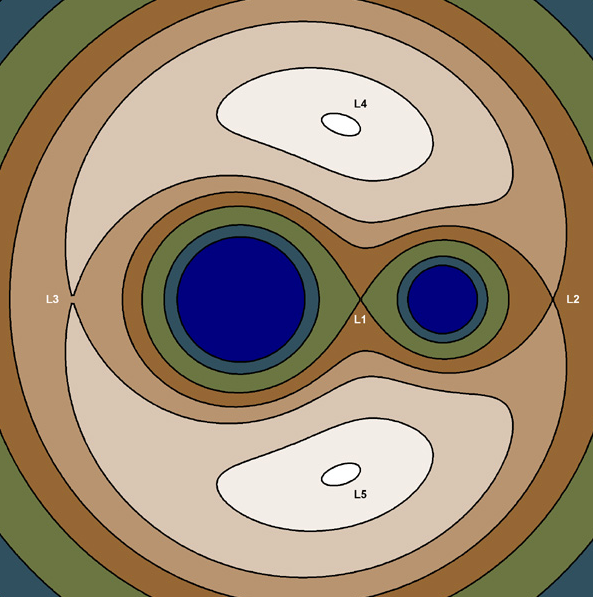
\includegraphics[width = 0.6\linewidth]{Chapters/Figures/equipotential.png}
    \caption{Roche lobes and equipotential surfaces of a binary system formed by normal star $M_1$ and a compact object $M_2$. $L_1, L_2,..., L_5$ are the Lagrange points of the system (Figure credit to Jeff Bryant)}.
    \label{roche}
\end{figure}

 
The process of the accretion onto compact objects turns out to be one of the most efficient mechanisms for converting gravitational potential energy into radiation. An order-of-magnitude calculation shows this readily. For a body of mass $M$ and radius $R_{\ast}$ the gravitational potential energy released by the accretion of a mass $m$ far away onto its surface is 
\begin{equation}
    \Delta E_{acc} = GMm/R_{\ast}
    \label{accretion}
\end{equation}

where $G$ is the gravitation constant. If the accreting body is a neutron star with radius $R_{\ast} = 20$ km, and the mass to be $M \sim M_{\odot}$, the solar mass, then the yield $\Delta E_{acc}$ is $6.63\times 10^{15}$ Joules per mass. This energy is released eventually mainly in the form of electromagnetic radiation. For comparison, consider the energy that could be released from a nuclear fusion reaction. The mass of a helium atom is about 0.8\% less than the mass of four hydrogen atoms which would combine to form a helium atom. This yields an energy of 
\begin{equation}
    \Delta E_{nuc} = 0.008 mc^2
    \label{fusion}
\end{equation}
where $c$ is the speed of light and $m$ is the mass of a helium atom. So we obtain $7.2 \times 10^{14}$ Joules per mass, which is about 10.9\% of the energy that the accretion yields. Equation~\ref{accretion} shows that the more compact of the acceting object, the greater the efficiency will be.\par

\subsection{The Components of the X-ray Binaries}
\subsubsection{The Compact Object}
Many properties such as the orbital period, magnetic field strength, and binary separation of an X-ray binary system depend on the nature of the compact object. Therefore, determining whether the compact object is a neutron star or a black is important to define those properties. A typical accreting neutron star system is an object the size of a small city (e.g. Norton) with a mass about that of the Sun but radiating in X-rays alone 10000 times the energy of the Sun. According to Equation~\ref{accretion}, the amount of accreting matter needed to produce this luminosity is about $10{^{-8}} M_{\odot}\mathrm{yr}^{-1}$. The binary nature of these systems sometimes allow us to determine the mass of the accretor by measuring the orbital velocity of the donor. The orbital velocity can be obtained by measuring Doppler shifts of the absorption lines, created by the donor.  \par

\subsubsection{The Donor}
An X-ray binary is classified as low-mass or high-mass according to the mass of the donor star. Usually, HMXBs contain a young, early-type (O, B or A), high-mass donor star which usually transfers mass by its stellar wind. LMXBs contain a late-type donor star or a white dwarf that usually undergoes Roche lobe overflow. 
%There are two non-physical approximations that give the the radius of the Roche lobe of the mass donor. They are functions of the binary mass ratio $q (=\dfrac{M_2}{M_1}) $ and separation $a$:

% \begin{

\subsubsection{The Accretion Disc}
From the previous section, we have seen that in an X-ray binary system, the accreting material usually has sufficient angular momentum to form an accretion disc. The gravitational energy gained by the gaseous matter is converted into heat, a fraction of which is converted into radiation, cooling down the accretion disc.\par 
Accretion discs in different binary systems have different properties. The discs in white dwarf binaries emit mainly in optical and ultraviolet while those in quasars and other active galactic nuclei emit radio emissions. Accretion discs that have characteristic temperatures $T\lesssim 10^6$K will radiate generally in the ultraviolet, optical and infrared \citep{King2002}. The temperatures of the inner and outer edges of an accretion disk can be determined by Keplerian orbital velocity

\begin{align}
     \dfrac{mv^2}{r} &= \dfrac{GMm}{r^2}\\
     v &= \sqrt{\dfrac{GM}{r}}
\end{align}
where $m$ is the accretion mass, $M$ is the mass of the accretor, $r$ is the distance from the accretion mass to the accretor,
and the equipartition theorem
\begin{equation}
    \dfrac{1}{2}mv^2 \sim \dfrac{3}{2}kT
\end{equation}
where $k$ is the Boltzmann constant.
For an X-ray binary system, the inner edge of the the accretion disk is could have a radius $R_{\mathrm{in}} \sim 10$ km and a temperature $T_{\mathrm{in}} \sim 10^7$ K. The outer edge of the disk could have $R_{\mathrm{in}} \sim 10^6 $ km and $T_{\mathrm{in}} \sim 10^3$ K \citep{King2002}. 
Figure~\ref{bhbinary} shows sketch of 16 Milky Way black hole binaries with companion stars and the accretion disks drawn to scale.\par


\begin{figure}[ht]
    \centering
    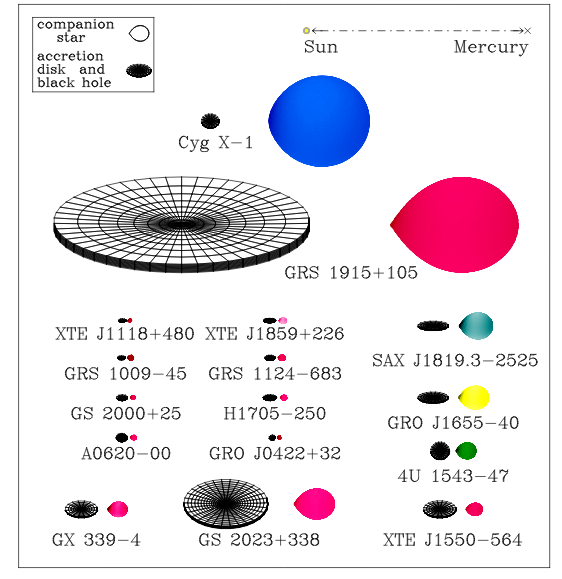
\includegraphics[width = 0.7\textwidth]{Chapters/Figures/BH_binaries.png}
    \caption{Scale drawings of 16 black hole binaries in the Milky Way (Figure by Jerome Arthur Orosz). The Sun–Mercury distance (0.4 AU) is shown at the top. The color of the companion star approximately indicates its surface temperature.}
    \label{bhbinary}
\end{figure}

\subsection{Maximum Luminosity during accretion: The Eddington Limit}

If the star has luminosity $L$ and radius $R$, the radiation pressure acting on an electron on the star's surface is
\begin{equation}
    -\dfrac{\sigma_T F}{c} = \dfrac{\sigma_T L}{4\pi R^2c},
\end{equation}
where $F$ is the incident radiation from the star and $\sigma_T$ is the Thomson cross section:
\begin{equation}
    \sigma_T = \dfrac{8\pi}{3}(\dfrac{e^2}{m_e c^2})^2 = 6.65 \times 10^{-25} \mathrm{cm^2}
\end{equation}
The maximum luminosity during a spherical accretion is attained when the inward gravitational force on a hydrogen atom balances out the outward pressure of radiation
\begin{equation}
    \dfrac{\sigma_T L_{\mathrm{edd}}}{4\pi R^2c} = \dfrac{GMm_p}{R^2}
\end{equation}
where $G$ is the gravitational constant, $c$ is the speed of light, $M$ is the mass of the gravitating body, $m_p$ and $M_{\odot}$ are the mass of the proton and the mass of the Sun. The luminosity at this point is called \textbf{Eddington luminosity},  also referred to as the Eddington limit 
\begin{equation}
    L_{Edd} = \dfrac{4\pi GMm_pc}{\sigma_0} = 1.26\times 10^{38} (\mathrm{M/M_{\odot}) erg/s} = 1.26\times 10^{31} (\mathrm{M/M_{\odot}) Joules/s}
    \label{eddington}
\end{equation}
Accretion discs are not spherical and often have additional stresses, related to turbulence, viscosity, shear and magnetic fields \citep{Pringle1981, Balbus1998}. Those additional stresses can counteract the radiation pressure along with gravity. Therefore, accretion discs may be somewhat brighter than the Eddington limit and radiate at super-Eddington luminosity. \par

\subsection{Jets}
Astronomical jets are collimated outflows moving at relativistic speed. The first jet discovered was of M87 in optical photographs from Lick Observatory by Heber Curtis in 1918. Figure~\ref{m87} shows later optical, radio, and X-ray images of M87 taken by the Hubble Space Telescope (HST), the Large Array radio telescope (VLA) and the Chandra telescope. The irregular, knotty structure in X-ray image of the jet is similar to that detected by radio telescopes and the Hubble Space Telescope. At the very left of the images we see the bright galactic nucleus harboring a supermassive black hole.\par 

\begin{figure}[ht]
    \centering
    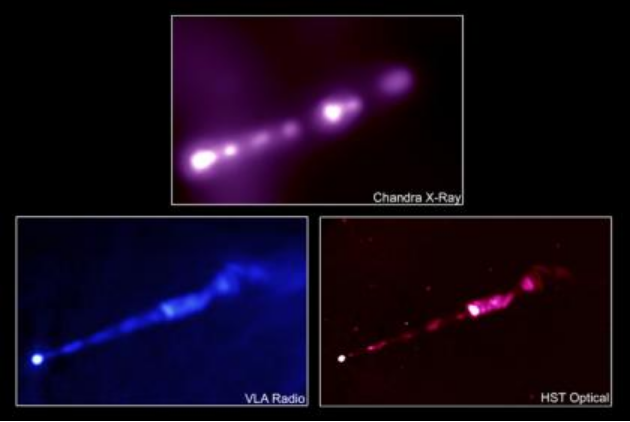
\includegraphics[width = 0.7\textwidth]{Chapters/Figures/M87jet.png}
    \caption{M87 jets observed by telescopes at X-ray, radio, and optical wavelengths. Top: X-ray image using Chandra telescope (NASA/CXC/MIT/H.Marshall et al.). Bottom left: Radio map take by the VLA (F. Zhou, F.Owen (NRAO), J.Biretta (STScI)). Bottom right: Optical image taken by HST (NASA/STScI/UMBC/E.Perlman et al.).  }
    \label{m87}
\end{figure}

Jets may consist of particles (mostly likely electrons and/or protons) moving at speeds close to the speed of the light (relativistic speed). The details of the formation of the powerful jets are still unclear. Jets can have significant impact on the surrounding matter. The jet that emanates from one galaxy can interact with the companion galaxy. This interaction may cause or inhibit the star formation.\par 

Inside the jet where the temperature is high, the collisions between atoms excite electrons into higher energy levels. When the electron decay back to its ground state in a very short of time (typically $10^{-8}$ s), it releases energy in the form of photon of a characteristic wavelength. This causes the bright emission lines in the spectrum. While it takes only $\sim 10^4$ K to completely ionize hydrogen, it is hard to completely ionize heavy elements such as iron and magnesium because they have many electrons. Thus only at very high temperature regions, such as the parts of the jet that are closest to the accretor of an X-ray binary system, would those heavy atoms be ionized to a higher degree. Magnetic field in the accretor causes those free high-speed electrons spirals around magnetic field lines of force, creating the radio, optical and X-ray knots \citep{Miller_2002}. Then electrons start to emit radiation as they accelerate in the magnetic field, which is called the \textbf{synchrotron radiation}. Another process that produces photons in the jets is  \textbf{Bremsstrahlung radiation}, which is radiation produced by a charged particle, undergoing acceleration. Bremsstrahlung radiation forms the continuum X-ray spectrum.



\section{Introduction to SS 433}

SS 433 is the first discovered microquasar. It is a smaller version of quasar that is composed of a compact object with a mass several times that of our sun and a companion star. SS stands for the initials of two astronomers, C.B. Stephenoson and N. Sanduleak, who compiled a list of emission-line objects \citep{Stephenoson1977}. SS 433 is the 433rd entry in that list. SS 433 is near the center of a supernova remnant called W50, a large nebula elongated in east-west direction. Figure~\ref{w50} shows W50, which has the shape similar to a conch. Due to the radio impact of W50, the coordinate of SS 433 was mistakenly identified several times. The realization that the radio, optical, and X-ray emissions are actually from the same object, SS 433, was reached by \cite{Clark1978}.\par

\begin{figure}[ht]
    \centering
    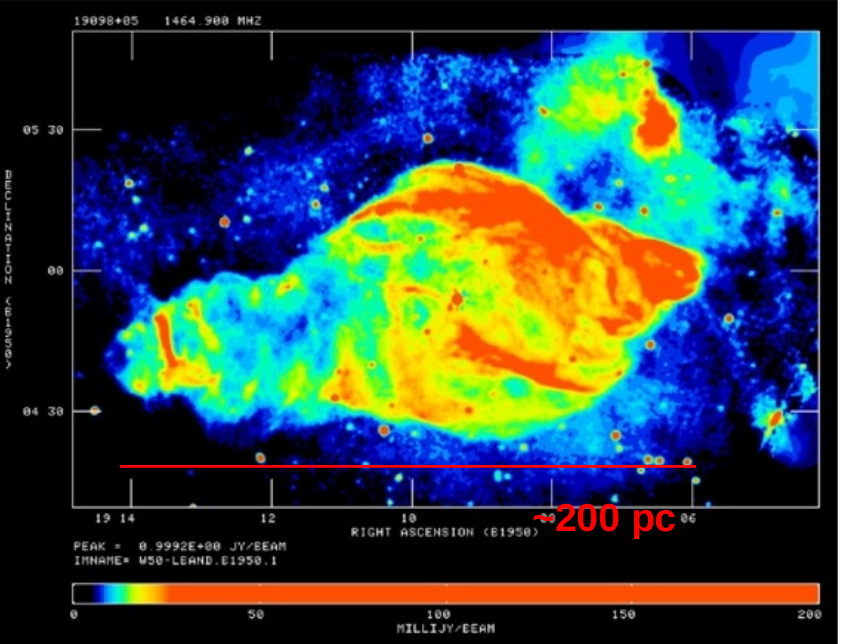
\includegraphics[width = .8\linewidth]{Chapters/Figures/w50.png}
    \caption{A radio map produced by VLA showing SS 433 as radio star surrounded by the shell of the W50 nebula. The big red dot near the center indicates SS 433 \citep{Dubner1998}.}
    \label{w50}
\end{figure}


\subsection{The moving lines}
SS 433 is one of the many emission-line objects showing very strong H$\alpha$ (the 3 to 2 transition in hydrogen) and neutral helium (He I) emission lines in the optical spectrum. Other than these emission lines, the spectrum of SS 433 contains many bright emission features at unfamiliar wavelengths. However, there are two other emissions for each rest line at abnormal wavelengths moving from one night to the next. The velocity of the changing motion is astonishing comparing to other binary systems. This caused the attention of Bruce Margon and his colleagues \citep{Margon1979}. They found that many other emission lines also have moving components. Each line's sets of components move in the same pattern (Figure~\ref{dopplershift}). It shows the smooth periodic motion of the pair of lines in opposite directions.

\begin{figure}[ht]
    \centering
    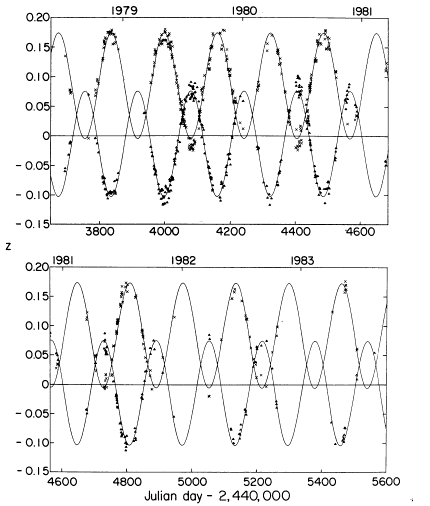
\includegraphics[scale = 0.6]{Chapters/Figures/dopplershift.png}
    \caption{Doppler shifts of SS 433 on 450 nights in the period 1978-1983. The period is the 164 days, showing the stability of the periodic motion of the jets. \citep{Margon1984}.}
    
    % The solid curve is a least-squares best fit to the kinematic model. The free parameters and their associated 1$\sigma$ uncertainties for this fit are $v/c = 0.2601\pm$0.0014, $\theta=19.80\degree \pm 0.18\degree$, $i = 78.82\degree \pm0.11\degree$, $P_p = 162.532 \pm 0.062$ days.
    \label{dopplershift}
\end{figure}

There were two conjectures associated with this motion of the lines if we assumed that it is due to the orbiting motion of two bodies. Firstly, the amplitude of the movement is enormous, which indicates a maximum velocity of about 50,000 km s$^{-1}$ in the redshifted and a minimum velocity of 30,000 km s$^{-1}$ in the blueshifted feature \citep{Margon1984}. From Kepler's law, in order to have such large velocity, the orbiting object in the binary needs to have a mass of about a billion times of the Sun. It is quite impossible that human did not detect such massive object in the galaxy \citep{seward_charles_2010}.\par 

Secondly, the average velocity of the motion is about 12000 km s$^{-1}$. Assuming a cosmological origin for this velocity (and using Hubble's constant which is $\sim$ 70 km/s/Mpc), SS 433 would be extremely far away from us (definitely extragalactic). However, the stationary emission lines are at a much lower velocity, which suggests that it is located within our galaxy \citep{seward_charles_2010}. 

\subsection{Relativistic jets}
The solution to solve the mystry of the `moving lines' is the \textit{kinematic model}
developed independently by \cite{Fabian1979} and \cite{Milgrom1979}. Abell and Margon fitted this model to the optical characteristics of SS 433 \citep{Margon1979}. The solid lines in Figure~\ref{dopplershift} is a least-squares best fit to the kinematic model. This model consists of a pair of jets of gas travelling in opposite directions at a relativistic speed of 0.26$c$ \citep{Margon1979}. Figure~\ref{geomtry_ss433} shows the geometry of the SS 433 system. Two jets precess about a common axis with the 164-day period. Therefore, the pair of jets vary their orientation respect to us from time to time, causing the observed Doppler velocity modulation. There are times when both jets are travelling perpendicular to our line of sight and then the moving lines appear to cross over in the spectrum (Figure~\ref{dopplershift}).\par 


\begin{figure}[ht]
    \centering
    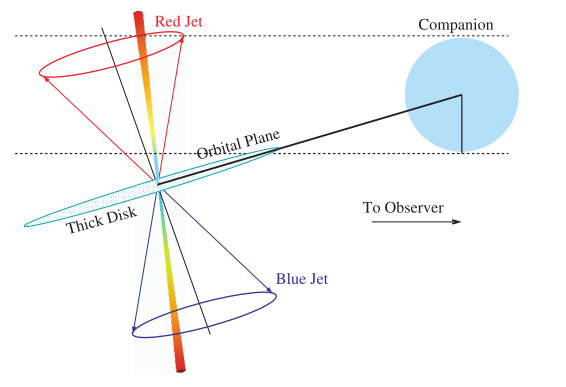
\includegraphics[width = 0.7\linewidth]{Chapters/Figures/geometry_ss433.png}
    \caption{Schematic geometry of the `kinematic model' of SS 433. This shows a pair of jets moving in opposite directions. The opening angle of the jet $\theta=19.80\degree \pm 0.18\degree$. The angle between the jet axis and the line of sight is $i = 78.82\degree \pm0.11\degree$. The period of the jet precession is $P_p = 162.532 \pm 0.062$ days \citep{Margon1984}. Figure from \citep{Lopez2006}.}
    \label{geomtry_ss433}
\end{figure}

At the times when both lines are crossing, the value of the redshift is not zero. It is due to the fact of special relativity. Imagine a object is travelling at an angle $\theta$ to our line of sight with velocity $v$. The component of this velocity toward us is $v\mathrm{cos}\theta$. According to the classical Doppler shift, when $v$ is small, any radiation emitted with a wavelength $\lambda_0$ will be observed by us at a wavelength $\lambda$ where
\begin{equation}
    \lambda = \lambda_0\left(1+\dfrac{v\mathrm{cos}\theta}{c}\right).
    \label{nonrelativistic_doppler}
\end{equation}
We notice that when $\theta = 90$, $\lambda = \lambda_0$, which means that when the object is moving perpendicular to us, there will be no Doppler effect. The observed wavelength shift (redshift) value is defined by 
\begin{equation}
    z = \dfrac{\lambda - \lambda_0}{\lambda_0} = \dfrac{v\mathrm{cos}\theta}{c}
\end{equation}
But when $v$ is very large, in the sense of a large fraction of the speed of light $c$, the effect of special relativity needs to be considered. The observed wavelength now becomes
\begin{equation}
    \lambda = \lambda_0 \dfrac{1 + \dfrac{v\mathrm{cos\theta}}{c}}{\left(1 - \dfrac{v^2}{c^2}\right)^{1/2}}
    \label{relativistic_doppler}
\end{equation}
Notice that Eq(\ref{relativistic_doppler}) reduces to Eq(\ref{nonrelativistic_doppler}) when $v \ll c$. \par 

This is called the \textbf{relativistic Doppler shift}. The principle is that if two clocks are synchronized and one is moving in a spacecraft relative to the other on the Earth at a large speed, the observer on the earth will observe the clock on the spacecraft slower compared to one on the Earth. This is called the \textbf{time dilation}, which is independent of the direction in which the spacecraft is travelling. The clock will appear to run slow no matter whether the spacecraft is travelling toward, away from you or perpendicular to the line of sight. For a spectral line, it is similar to an atomic clock in the sense that it appears to run ``slow'' when it moves at relativistic speed. This dilation applies to the duration between two successive light wave crests emitted by the source. Therefore, the observed wavelength is always greater than the emitted one. The factor by which it does run slow is the $\left(1 - \dfrac{v^2}{c^2}\right)^{1/2}$ shown in Equation ~\ref{relativistic_doppler}, which is called the \textit{Lorentz gamma factor}. According to Equation~\ref{relativistic_doppler} and Figure~\ref{dopplershift} which shows $z(\theta = 90\degree) = 0.035$, the velocity of the jet is 0.26$c$.\par
As seen from the earth the jet that is more Eastern oriented approaches us most of the time, we called it the blue jet. Similarly, we call the other jet, which is more Western oriented and receding from us most of the time, the red jet. 


\subsection{SS 433 as an X-ray binary} 
Combining the angular periodicity of the corkscrew structure projected on the plane of the sky produced by the precession of the jet axis, and the jet velocity of 0.26c, the distance to SS 433 is determined to be 5.5 kpc \citep{Blundell2004}. 
From the spectrum of SS 433, in addition to the fast moving emission lines from the jet, there are also slowly moving features from the donor star that have a period of 13.1 days \citep{Crampton1980}, which is the period of the this binary system. Tentative detections of donor's spectrum have been made \citep{Hillwig2004} showing that the mass donor is probably an early-typed A supergiant star (A3-7 I) with a temperature between 7,500 to 10,000 K. Over an estimate of forty years, the range of the mass of the compact object have spanned from 1 to 30 solar masses \citep{Bowler2018}, from neutron star to massive stellar black hole. It is still unclear which is correct although recent studies \cite{Lopez2006} and \cite{Bowler2018} point to a black hole of mass of $15 \pm 2 M_{\odot}$. The dilemma of determining the mass ratio could be resolved if the spectrum of the companion could be identified and its orbital velocity curve measured. In \cite{Bowler2018}, the ratio of the mass of compact object to the mass of the companion star is calculated to be about 0.7 based on the shape of the He I stationary lines. \par

The absolute magnitude of SS 433 is $-6^m.28 < M_V < -5^m.4$ \citep{Goranskij2011}, the interstellar extinction $A_v$ in the direction of SS 433 is $7^m.3 - 8^m.3$ \citep{Cherepashchuk1982} and distance of the system $d$ is 5.5 kpc. We can then predict the apparent V-band magnitude $m_V$ of the donor according to the distance modulus formula
\begin{equation}
    m_V = M_V - 5 + 5\mathrm{log}_{10}(d) + A_V.
\end{equation}
The predicted apparent V-band magnitude is calculated to be about $15^m.9$. However, the observed apparent V-band magnitude is $13^m$ \citep{Cherepashchuk1982}. This discrepancy suggests that SS 433 exceeds the Eddington luminosity.\par


\subsection{The Uniqueness of SS 433}
Many more microquasars have been discovered since the discovery of SS 433. Most of them are black hole X-ray transients, whose intensities vary a lot during a short amount of time. However, SS 433 is the only source that has a pair of persistently precessing jets. Furthermore, it is the only jet source that shows spectral lines from many different elements \citep{Margon1980}. Thus, we know that SS 433's jet is made of baryonic matter, i.e. heavy particles, such as protons and neutrons \citep{seward_charles_2010}. The moving lines produced by those elements indicate the precise velocity (0.26$c$) of the jet, and line diagnostics give the temperature and density.\par 

The observed super-Eddington luminosity is quite likely the result of much higher mass transfer rate in SS 433 ($10^{-4} M_{\odot} \mathrm{yr}^{-1}$) than other known HMXBs \citep{Van_den_heuvel1981}. This may imply that SS 433 is a short-lived binary system, with a lifetime of a few tens of thousands of years only \citep{seward_charles_2010}. That may be a reason why microquasar like SS 433 is so rare in the universe.




\subsection{X-ray Observations of SS 433}
The early X-ray observations (e.g. using EXOSAT/GSPC, ASCA) showed that the strongest X-ray emission line was caused by highly ionized iron which lost all but one of its electrons (Fe {\sc xxvi}) \citep{Watson1986}. This indicates that the X-ray emission must originate in inner region of the system, which has a high temperature of $50-100 \times 10^6$ K \citep{fabrika2004}. The total luminosity of the X-ray emission is $L_x$ is from $3 \times 10^{28} - 10^{29} \mathrm{J/s}$ \citep{fabrika2004}. X-ray emission is strongly variable. It depends on the orientation of the accretion disk and jets (precessional phase) and the effects of eclipses of the optical star (orbital phase). The detected X-ray iron lines in those observations are from the Eastern (approaching) jet but lines are absent from the Western (receding) jet \citep{fabrika2004}. The reason could be the receding jet is eclipsed by the accretion disk (indicated in Figure~\ref{geomtry_ss433}).\par

Previous studies on the X-ray observation of SS 433 have been published by \cite{Marshall2002}, \cite{Lopez2006}, and \cite{Marshall2013}, focusing on studying SS 433 with Chandra High Energy Transmission Grating Spectrometer (discussed in Chapter 2). \cite{Marshall2002} resolved the X-ray lines, detected fainter lines than previously observed. \cite{Lopez2006} utilized an eclipse to determine the radius of the companion star, which is $1.08 \times 10^{12} $ or $15.50 R_{\odot}$. \cite{Marshall2013} observation used an eclipse to conclude that the X-ray spectra were remarkably consistent before and after the eclipse and eclipsed emission is hard. It also suggests that the directions of the Eastern and Western jets are independently determined or affected by the environment. Figure~\ref{HETG2002} shows Chandra's high spectral resolution, which allows studying the X-ray emission lines of SS 433 in more details than was possible earlier. In most of the Chandra HETG observations, there are many lines from the approaching jet and a few lines from the receding jet. The strongest line was a helium-like line of iron Fe \rncaps{25} \citep{Marshall2002, Marshall2013}.


\begin{figure}[h!]
    \centering
    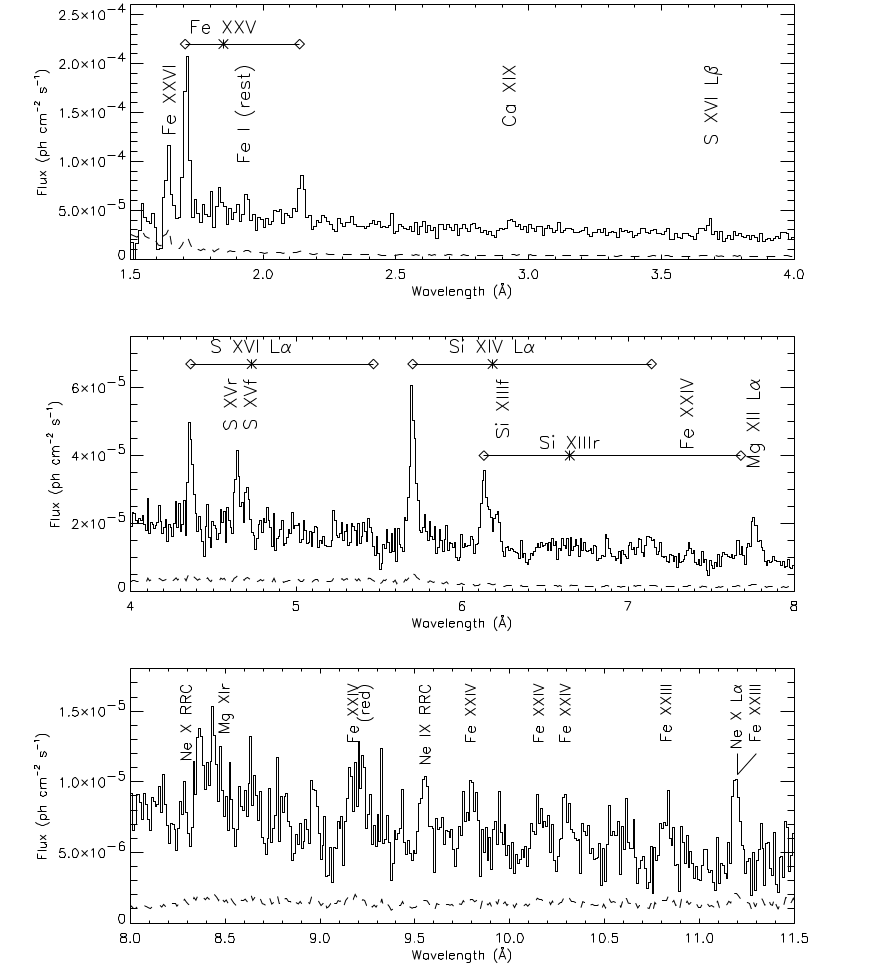
\includegraphics[width = \linewidth]{Chapters/Figures/HETG2002.png}
    \caption{Chandra HETGS spectrum of SS 433 obtained at precession phase 0.51 and orbital phase 0.67. Most of the lines are from the blue jet. The strongest lines are marked with horizontal bar indicating the positions of the red-shifted, blue-shifted (diamonds) and rest wavelengths (asterisks) (original diagram by \citep{Marshall2002}.}
    \label{HETG2002}
\end{figure}

Three Si {\sc xiii} lines (Si {\sc xiii} triplets) whose rest wavelengths at 6.2 \AA\ region are used to determine the electron density. These three lines are called  Si {\sc xiii}r,  Si {\sc xiii}i, and  Si {\sc xiii}f. Letter r, i, and f indicate ``resonance'', ``intercombination'', and ``forbidden'' respectively \citep{porquet2010}. Figure~\ref{HETG2002} shows lines from Si\rncaps{13}f and Si\rncaps{13}r. They are the most intense lines of helium-like ions (``triplet''). They correspond to transitions between n= 2 shell and n= 1 ground-state shell \citep{porquet2010}. In Figure~\ref{rif}, resonance is shown as $w$, which is an electric dipole transition, intercombination as $x + y$, which is a magnetic quadrupole transition and forbidden as $z$ transition, which is a relativistic magnetic dipole transition \citep{porquet2010}.



\begin{figure}[h!]
    \centering
    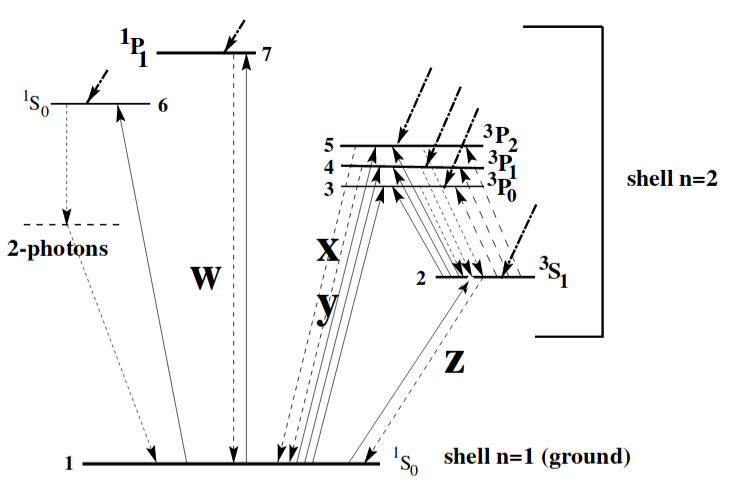
\includegraphics[width = 0.7\linewidth]{Chapters/Figures/rifgraph.png}
    \caption{Simplified level scheme for helium-like ions w (or resonance) x; y (or intercombination), and z(or forbidden): resonance, intercombination, and forbidden lines, respectively \citep{porquet2010}.}
    \label{rif}
\end{figure}







\section{Some unanswered questions about the jets of SS 433}
Previous detailed spectral modeling shows that there is a broad range of temperatures in the outflow, with different ionization states sampling different regions of the jets. Although previous observations provided valuable insights about the jets, none of these observations were designed to follow the source while it was coming out of an eclipse. Therefore, using an eclipse of the compact object by the donor, our 96 ksec long observation tracking the accretor coming out of the eclipse can map out the spatial variations of the physical properties of SS 433’s X-ray jet. Splitting the spectrum from the long observation into 5 parts and analyzing them enable us to see how the flux of the emission lines, redshifts of the jets, and other physical properties of the jets change over the long observation. These information will give us insights about which regions of the jets produce certain kind of elements. What is more, the 20 ksec short observation taken before an eclipse enables us to check that the changes in line properties during the main observation were indeed due to the eclipse and not due to any significant changes in the intrinsic accretion in/outflows. Previous observations were all taken when the Western jet (which points away from us most of the time) was receding from us, which causes the Western jet being too faint to analyze. Our observation, instead, were designed to take during the epochs when the Western jet was closest to our line-of-sight and hence easiest to observe due to Doppler beaming. \cite{Marshall2013} observation suggests that the Doppler shifts change by $\gtrsim 3000 km \mathrm{s^{-1}}$ during the day. This suggests that the two jets might be moving independent to each other. Therefore, we would also like to check whether there was another abnormal change of the redshift during our observation. \par 




% Knowing more about which lines are occulted by the eclipse will help us understand better about the geometry of the system, which is helpful to estimate the size of the companion star. Those information would further benefits to estimate the masses of both the accretor and the donor. 




 













% \subsection{The Radio jets and W50}
% SS 433 is a very bright radio star, whose central radio source radiates at a level of about 1 Jy (a non-SI unit non-SI unit of spectral flux density, equivalent to about $10^-26$ watts per square meter per Hz) at centimeter wavelengths. The maximum of the radio emission occurs at a distance of $\sim 10^15$ cm from the source \citep{Hjellming1981}, the same place where the strongest optical jet line emission originates. The brightness of the radio jet decreases to a distance of $\sim 10^17$ cm away from the source and became invisible beyond this distance until a distance of $\sim 10^{20}$ cm. At this place, the jets are decelerated and the large-scale X-ray jets are observed together with an increased intensity of the radio emission \citep{}.








%\subsection{The disc and Precession Mechanism}

%-----------------------------------

%----------------------------










  \chapter{The Chandra Telescope and Analyzing X-ray Spectra Obtained with Chandra}
\section{Introduction to The Chandra X-ray Observatory}
The Chandra X-Ray Observatory (CXO) is a space observatory launched by NASA's Space Shuttle Columbia on July 23, 1999 with Col. Eileen Collins commanding. Chandra is the X-Ray component of NASA's four Great Observatories. The period of the Chandra is about 3809.3 minutes. The other three components are the Hubble Space Telescope, the late Compton Gamma-Ray Observatory and the Spitzer Space Telescope. Since the Earth's atmosphere absorbs the vast majority of X-rays coming from space, an X-ray telescope on the earth can not detect those X-rays. Therefore, space-based telescopes, like Chandra, are required to make the X-ray observations of astronomical objects. Chandra's spatial and spectral resolutions are order-of-magnitude better than previous X-ray telescopes \citep{ChandraMSFC}. Thanks to advances in technology, the Chandra telescope is sensitive to X-ray sources 100 times fainter than any other previous X-ray telescope.  \par

\subsection{Main Components of the Chandra Telescope}
Chandra consists of a spacecraft and a telescope/science-instrument payload. The observatory has four main components: The High Resolution Mirror Assembly (HRMA), the Aspect System, the Science Instruments (SIs) at the focal plane and the Transmission Gratings. See Fig.~\ref{fig:chandratelescope} for a diagram of the Chandra X-ray Observatory with main components labeled \citep{Harbaugh2017}. The SIs includes the Advanced CCD Imaging Spectrometer (ACIS) \citep{canizares2003} and the High Resolution Camera (HRC) . The Objective Transmission Gratings include High Energy Transmission Grating (HETG) \citep{Canizares2000} and Low Energy Transmission Grating (LETG) \citep{Brinkman2000} which together cover the energy range from $\leq 0.1$ to 10 keV.\par 

\begin{figure}[ht!]
\centering
  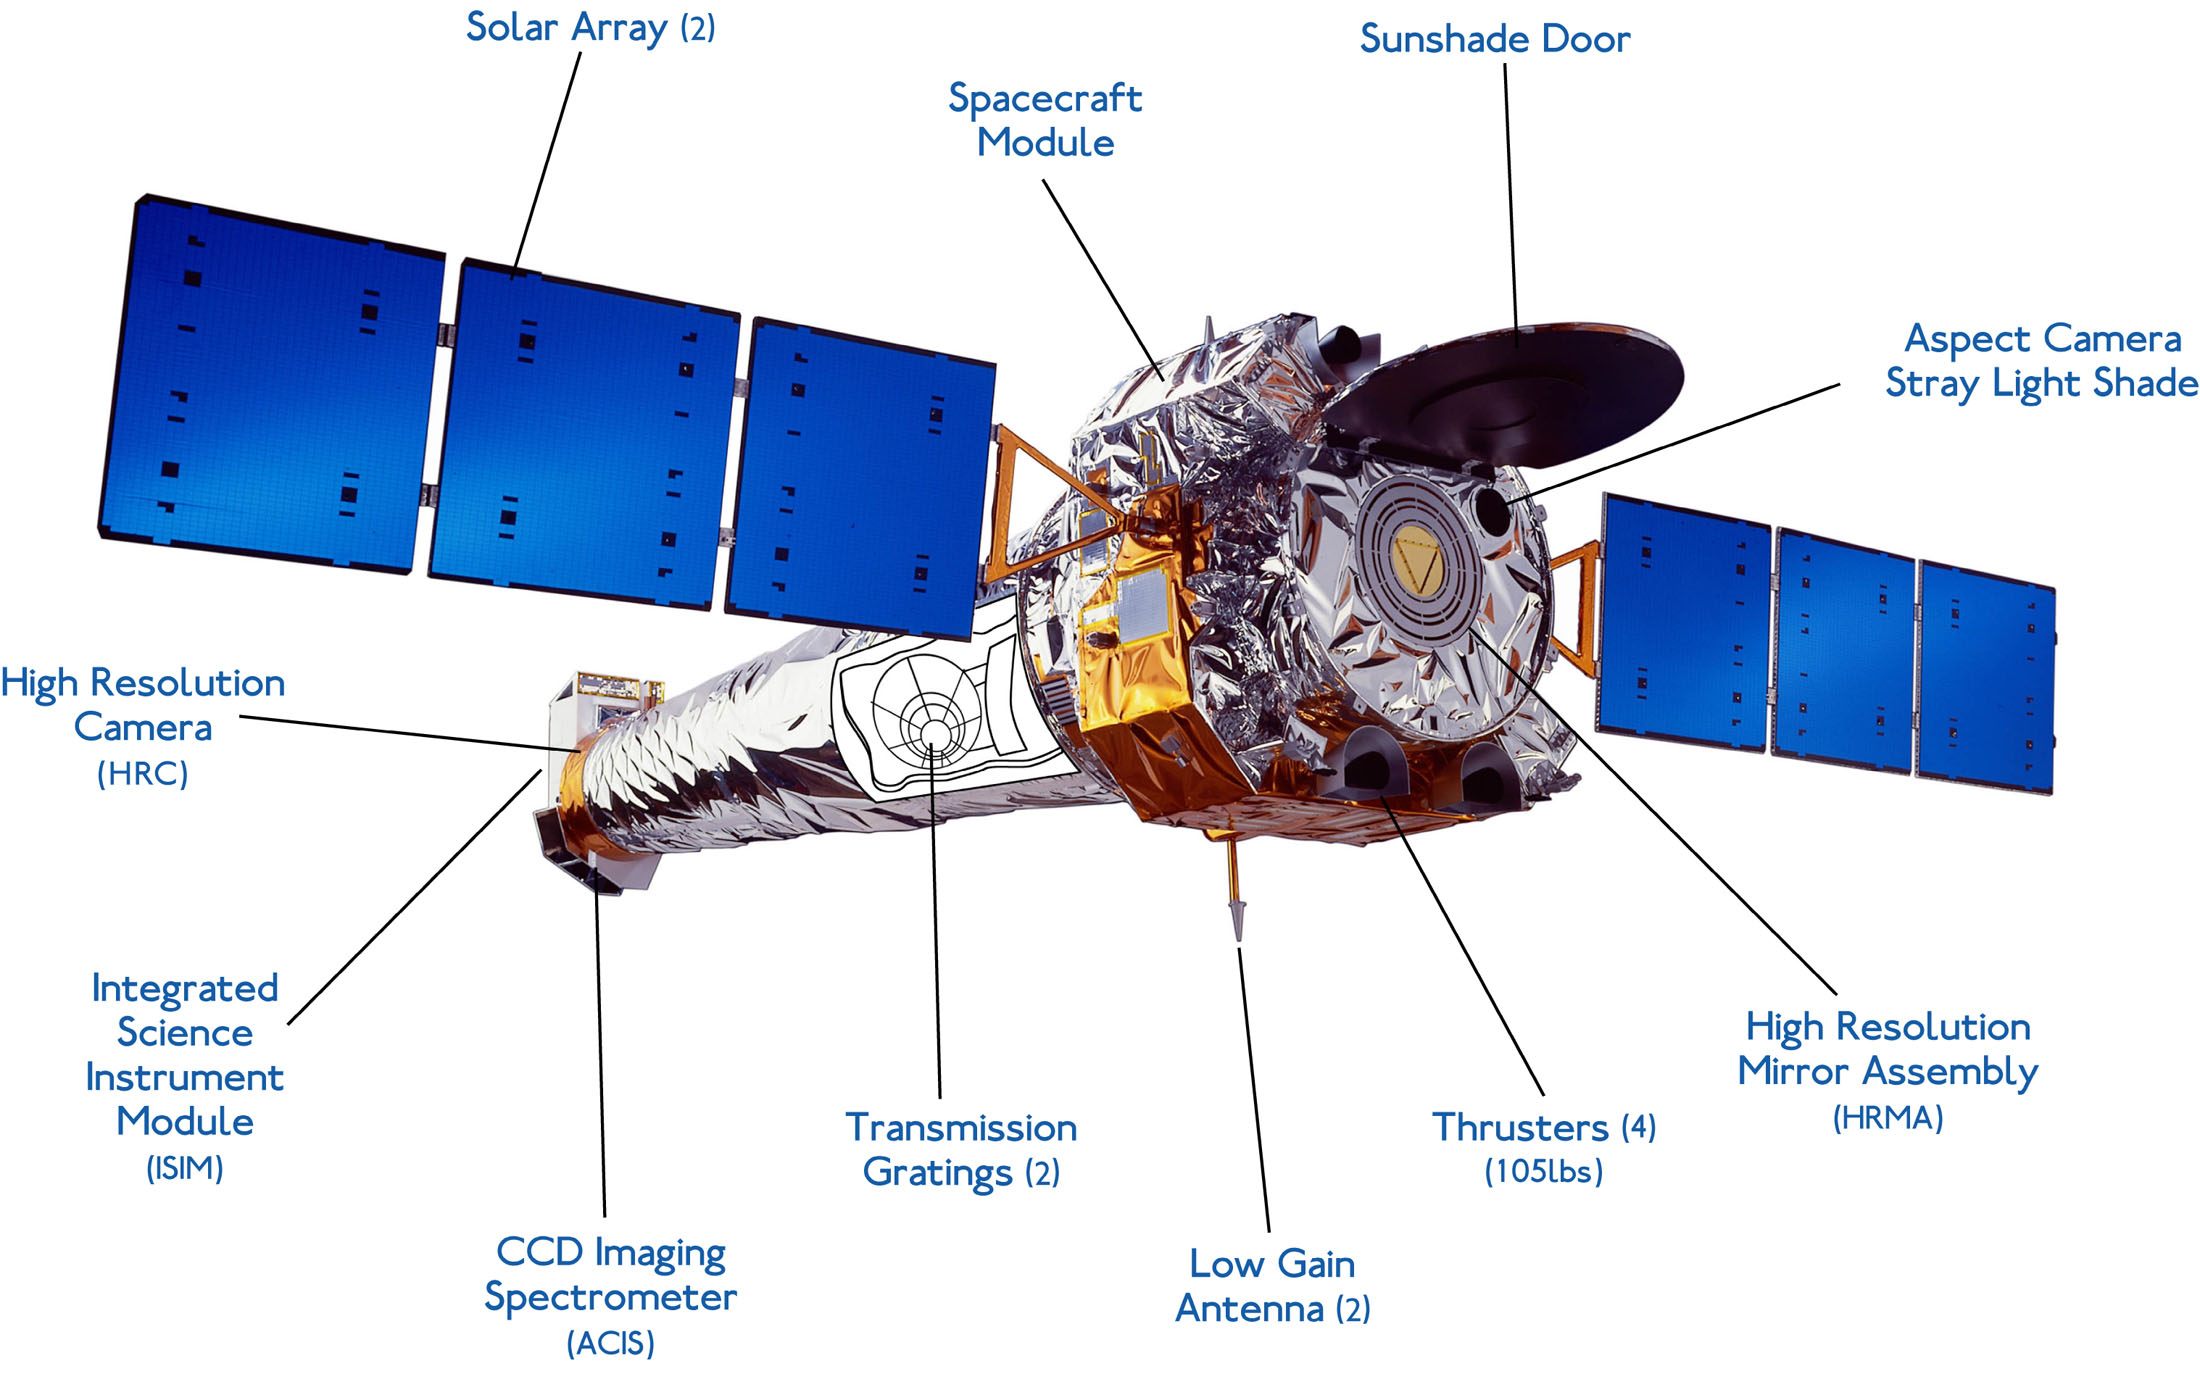
\includegraphics[width = \linewidth]{Chapters/Figures/chandra_full.jpg}
  \caption{The Chandra X-ray Observatory with main components labeled \citep{Harbaugh2017}}
  \label{fig:chandratelescope}
\end{figure}


\subsubsection{High Resolution Mirror Assembly (HRMA)}
The HRMA produces images with a half-power diameter of the point spread function of $<$ 0.5 arcsec. The HRMA consists of a nested set of four paraboloid-hyperboloid, grazing-incidence X-ray mirror pairs, with the largest having a diameter of 1.2 m. The effective focal length is 10 m. See Fig~\ref{fig:HRMA} for the sectional view of the HRMA of Chandra. X-rays that hit the mirror at grazing angles are reflected like a pebble skipping across a pond.\par

\begin{figure}[ht]
\centering
  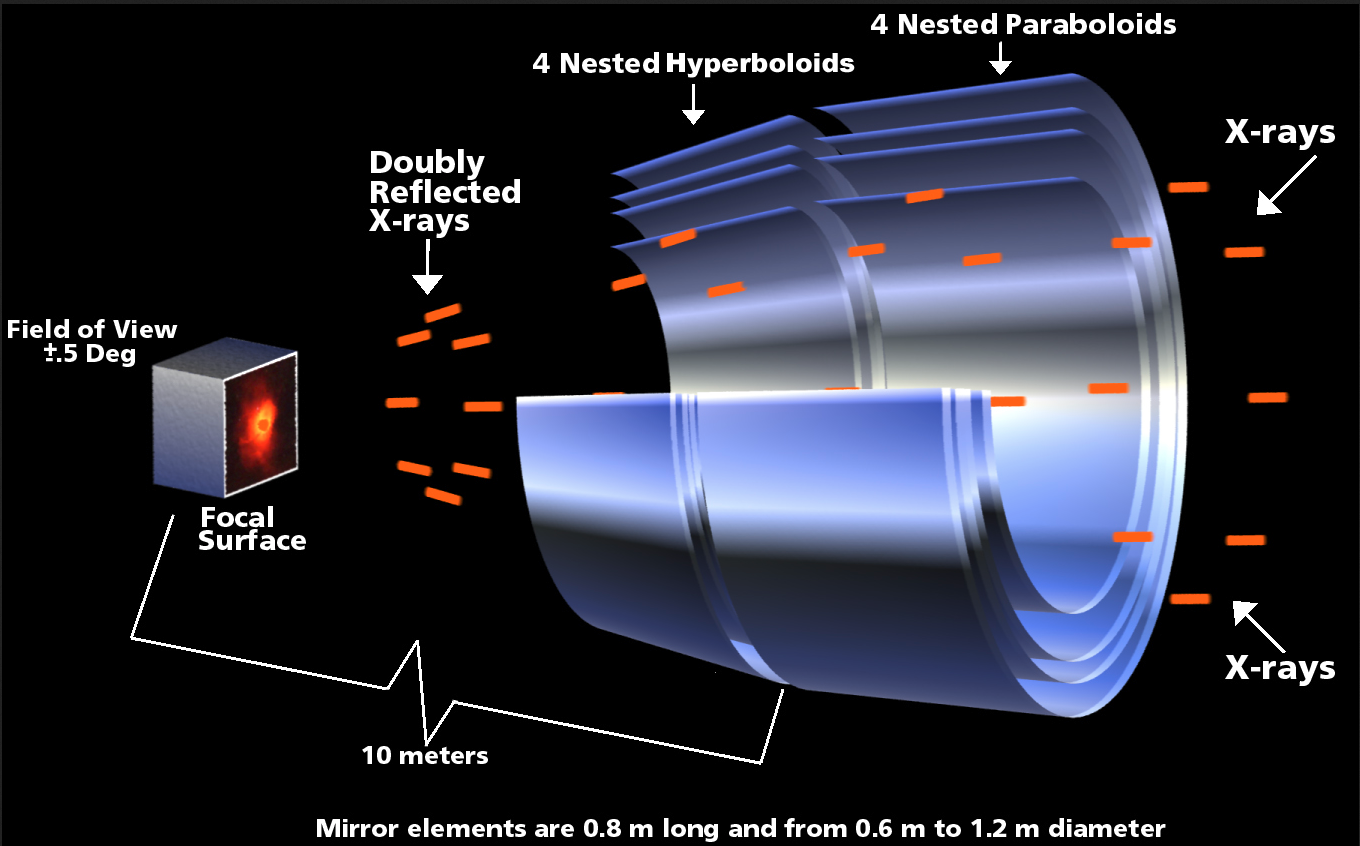
\includegraphics[width = \linewidth]{Chapters/Figures/paraboloid_hyperboloid_mirror.png}
  \caption{This cutaway illustrates the design and functioning of the High Resolution Mirror Assembly (HRMA) on Chandra \citep{NASA2009}.}
  \label{fig:HRMA}
\end{figure}


\subsubsection{The Science Instrument Module (SIM)}
The SIM contains the two detectors - the ACIS and the HRC. ACIS is composed of two CCD arrays, a 4-chip array, ACIS-I (16'$\times$16'), and a 6-chip array, ACIS-S (8'$\times$8') (See Figure \ref{fig:ACIS}).   


\begin{figure}[ht]
\centering
  \includegraphics[scale = 0.5]{Chapters/Figures/acis_def_chips_2.png}
  %\includegraphics[width=\linewidth]{acis_def_chips_2.png}
  \caption{A schematic drawing of the ACIS focal plane, not to scale \citep{ChandraMSFC}. ACIS-I and ACIS-S layout showing the imaging and spectroscopic arrays. The default aimpoints are marked with an x.}
  \label{fig:ACIS}
\end{figure}


\begin{figure}
    \centering
    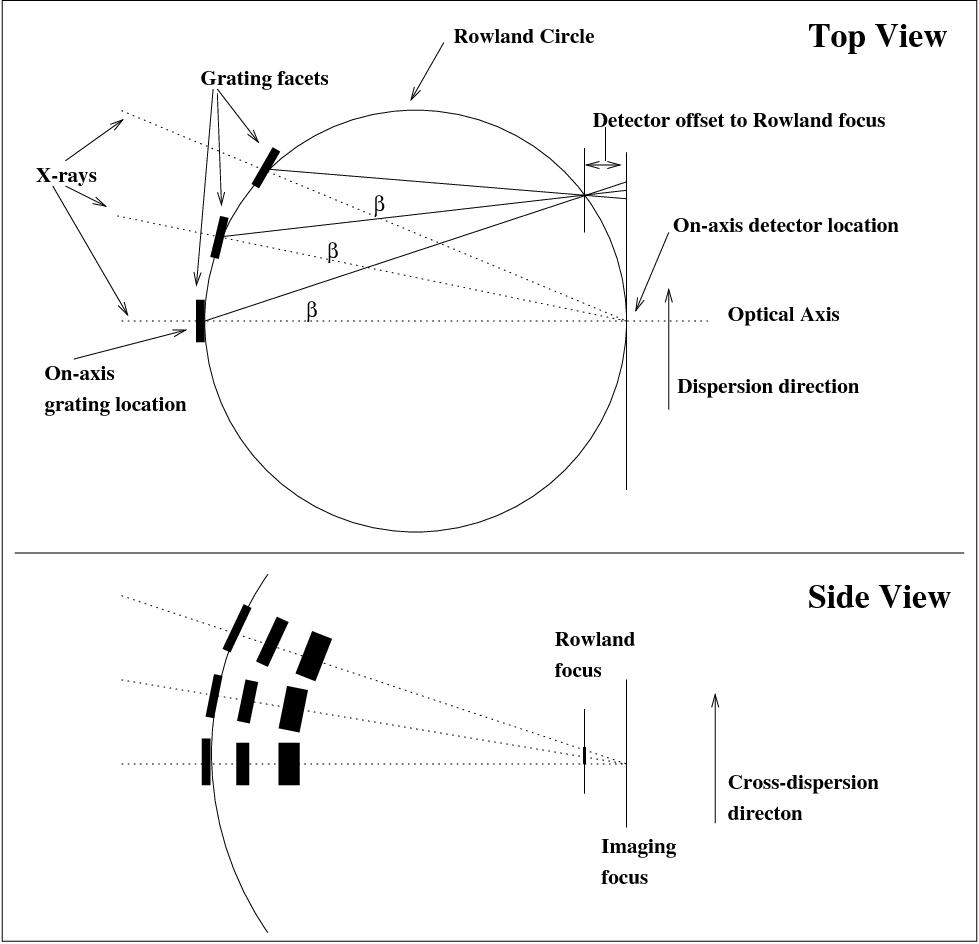
\includegraphics[width = 0.8 \linewidth]{Chapters/Figures/rowland.png}
    \caption{The Rowland geometry is shown schematically. In the ``Top'' view, the diffraction angle is $\beta$. The geometry is such that converging rays are diffracted at a specific angle by the gratings (which are located on the Rowland circle). Then the rays converge to a point that is also on the Rowland circle. The dotted lines show zeroth-order rays, which will be focused at the middle point of the other side of the Rowland circle. The solid lines represent the grating-diffracted first-order rays. The bottom panel (``Side'' view) looks along the dispersion direction at rays from a set of gratings arranged perpendicularly to those in the ``Top'' view. Since the converging rays have not yet reached the imaging focus, the spectra are extended perpendicular to the dispersion direction by less than 100 microns \citep{ChandraMSFC}.}
    \label{rowland}
\end{figure}


ACIS-I is usually better for direct imaging, and the ACIS-S is better suited for spectroscopy with the High-Energy Transmission Grating system. The CCDs detect X-ray photons individually and records their position on the detector, energy and arrival time. \par 



\subsubsection{The High Energy Transmission Grating (HETG)}

The HETG works with the High Resolution Mirror Assembly (HRMA) and a focal-plane imager for high resolution spectroscopy. The complete instrument is called the High-Energy Transmission Grating Spectrometer (HETGS). The HETGS achieves high resolution spectra (with $E/\Delta E$ up to 1000) between 0.4 keV and 10.0 keV energy range \citep{ChandraMSFC}. Standard processing of an HETG system observation produces spectrometer information products: PHA (Pulse Height Amplitude, the raw spectrum), ARF (Ancillary Response File) and RMF (Response Matrix File), the instrument calibration files). The HETG consists of two sets of grating assemblies - the High Energy Grating (HEG) and the Medium Energy Grating (MEG). The HEG diffracts X-rays from only the two inner mirror shells and the MEG diffracts X-rays from only the two outer mirror shells. \par
The HETGS-faceted Rowland design is shown in Figure~\ref{rowland}. The Rowland geometry of the grating plate and spectroscopic arrays minimize dispersed image aberrations so as to maintain the telescope's focal properties in the dispersion direction. As a result, Rowland geometry contributes to improved spectral resolution \citep{ChandraMSFC}. 


\begin{figure}[ht!]
\centering
  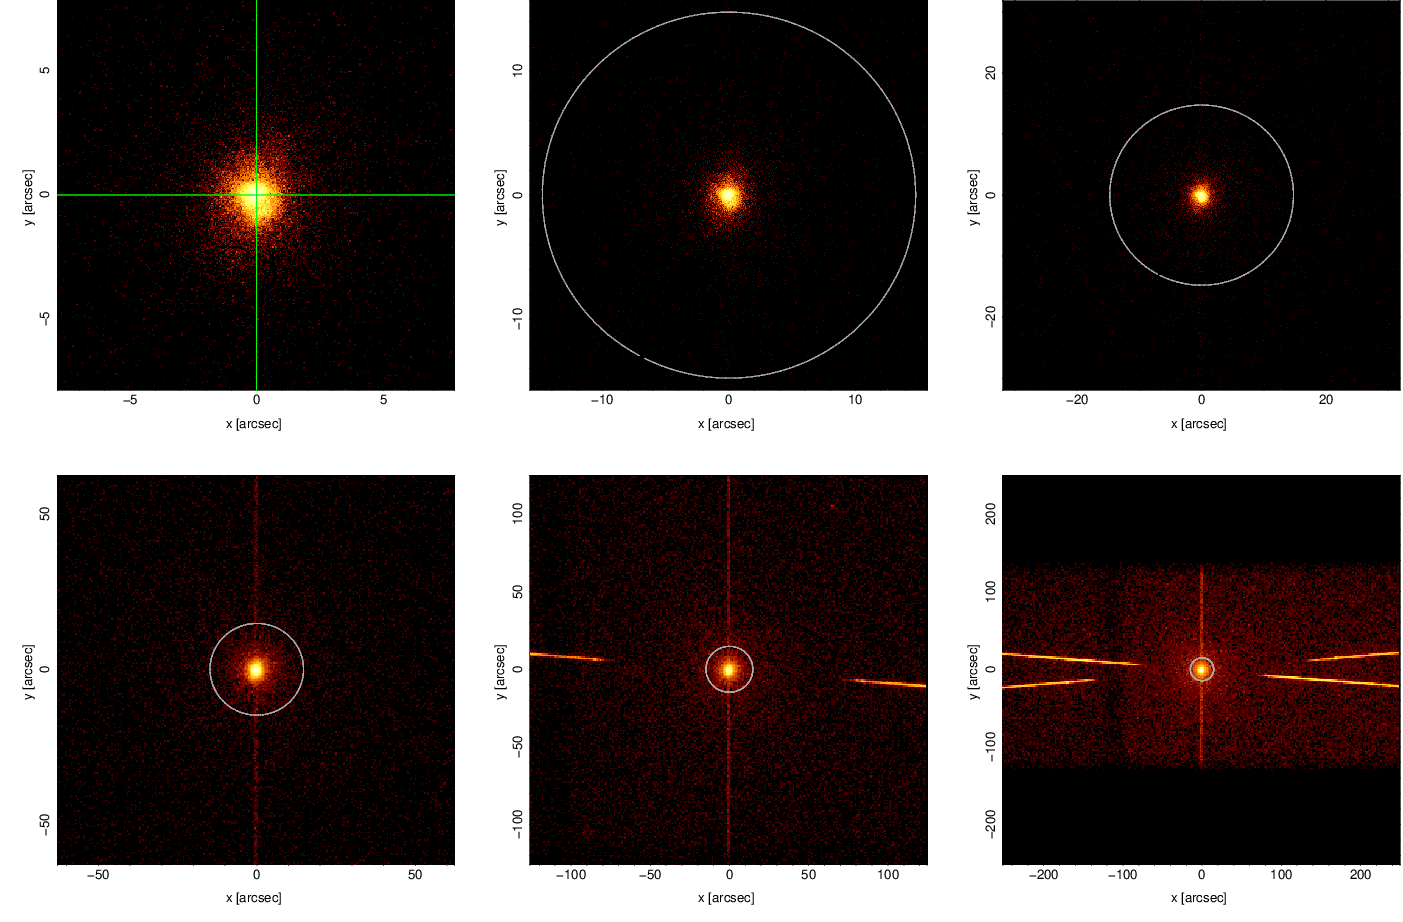
\includegraphics[scale=.3]{Chapters/Figures/X_orders.png}
  \caption{The top panel shows the bright zeroth order. The bottom panel shows the HETGS diffracted X pattern, yielding the first-order spectrum. }
  \label{xpattern}
\end{figure}

Figure~\ref{skyfield} shows the MEG and HEG spectra forming an ``X'' pattern. The bright zeroth-order image is visible at the aim point. The opening angle between the MEG and HEG is 9.96$\degree$. The first order (minus and plus) is followed by the zeroth order along the arms and so on. The spectroscopic array spans approximately $8'\times 48'$ of the sky. Wavelengths are assigned depending on how far the events are from the zeroth-order image. If X-rays of wavelength $\lambda$ hit the transmissions gratings and are diffracted (in one dimension) by the dispersion angle $\beta$, then according to the grating equation, we have
\begin{equation}
    sin\beta = m\lambda/p
\end{equation}
where $m$ is the integer order number and $p$ is the spatial period of the grating lines.
The HEG range is 15 - 1.2 \AA (0.83 -10.0 keV). The MEG range is 31 - 2.5 \AA (0.4 - 5 keV).\par

The HETG support structure (HESS) is a circular aluminum plate that is 110 cm in diameter and 6.35 cm thick \citep{ChandraMSFC}. HESS swings on and off depending on whether the images needed to be dispersed or not. There are 336 grating facets mounted on the HESS, each about 25 mm square \citep{ChandraMSFC}. Figure~\ref{hess} shows front and side view of the HESS. The two outer annuli have 192 MEG gratings and the two inner annuli have 144 HEG gratings. Every grating within one ring is mounted in the same direction such that X-rays coming to the gratings on the same ring will diffract at the same angle. The two sets of gratings are mounted with at different angles so that the dispersed images from the HEG and MEG will form a shallow X centered at the undispersed (zeroth order) position. A detailed schematic layout of HETGS is shown in Figure~\ref{hetgs}.\par 


\begin{figure}
    \centering
    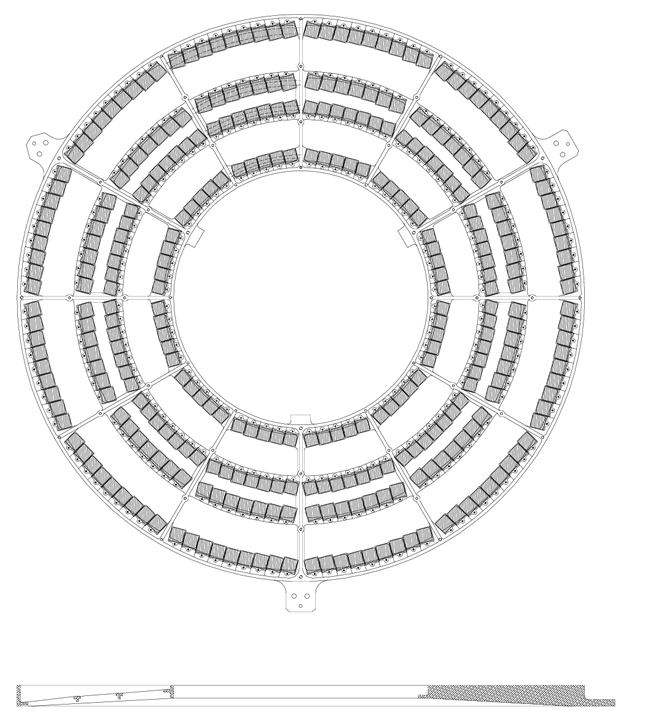
\includegraphics[width = 0.5\linewidth]{Chapters/Figures/hess.png}
    \caption{The upper and the lower figures show the front and the side view of the HESS, respectively. The front view is seen from the view of X-rays; the X-ray intercept with the grating facets as they leave the HRMA. In the side view, the left part shows the four support rings that are in different planes due to the Rowland curvature \citep{ChandraMSFC}.}
    \label{hess}
\end{figure}

\begin{figure}
    \centering
    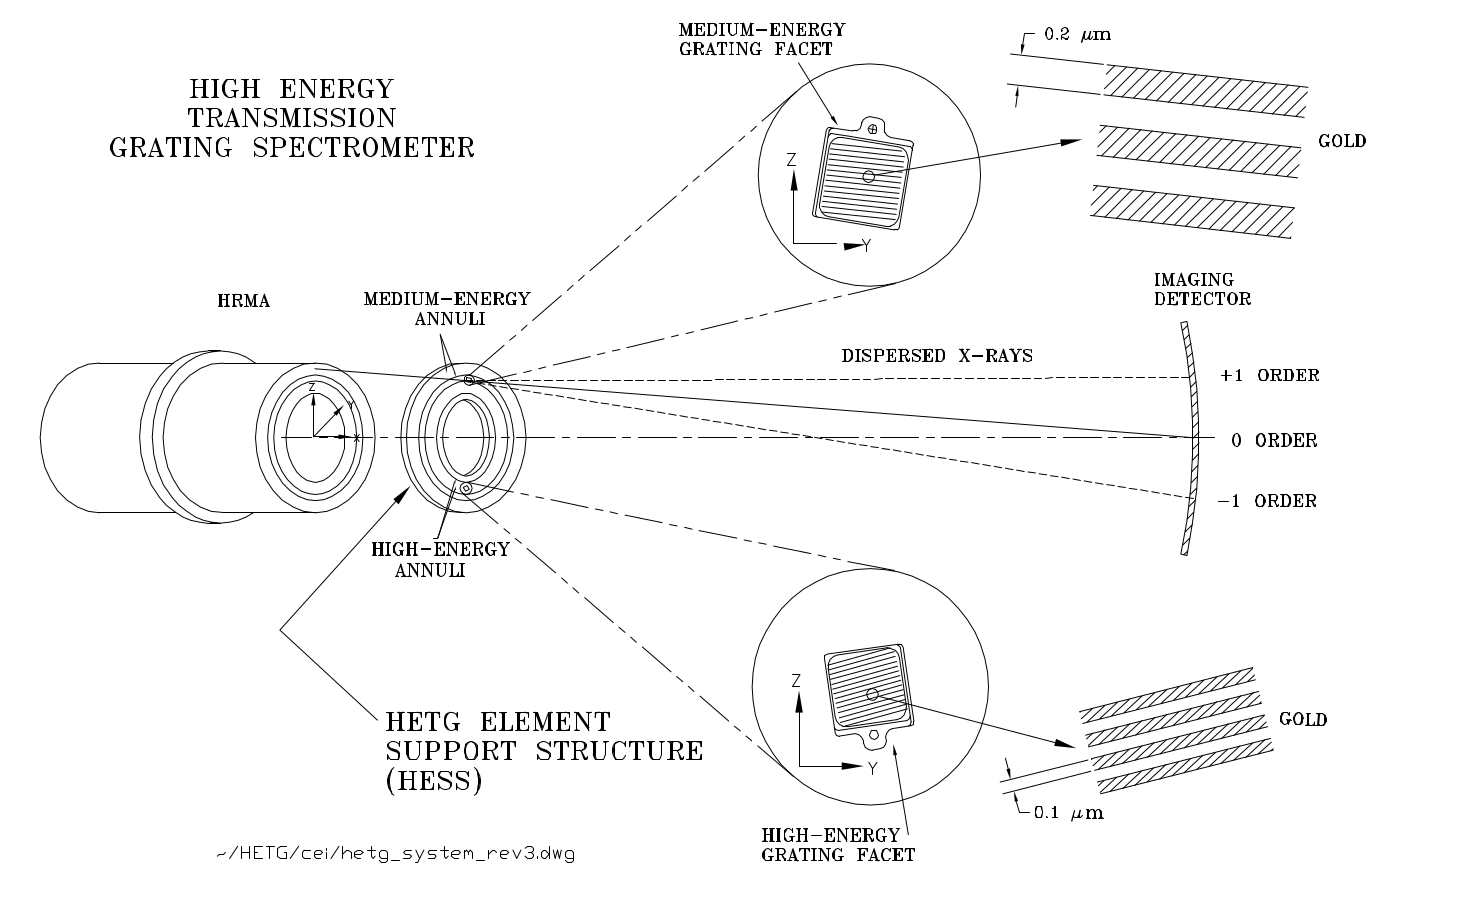
\includegraphics[width = 0.6\linewidth]{Chapters/Figures/hetgs.png}
    \caption{A schematic layout of the High Energy Transmission Grating Spectrometer \citep{ChandraMSFC}.}
    \label{hetgs}
\end{figure}

The HETG grating facets are made of electro-plated gold bars supported on a polyimide substrate. Figure~\ref{facet} shows a life-size model of the HESS with a few grating facets on it. This unit is currently in Dr. Herman Marshall's lab in MIT Kavli Institute.



\begin{figure}
    \centering
    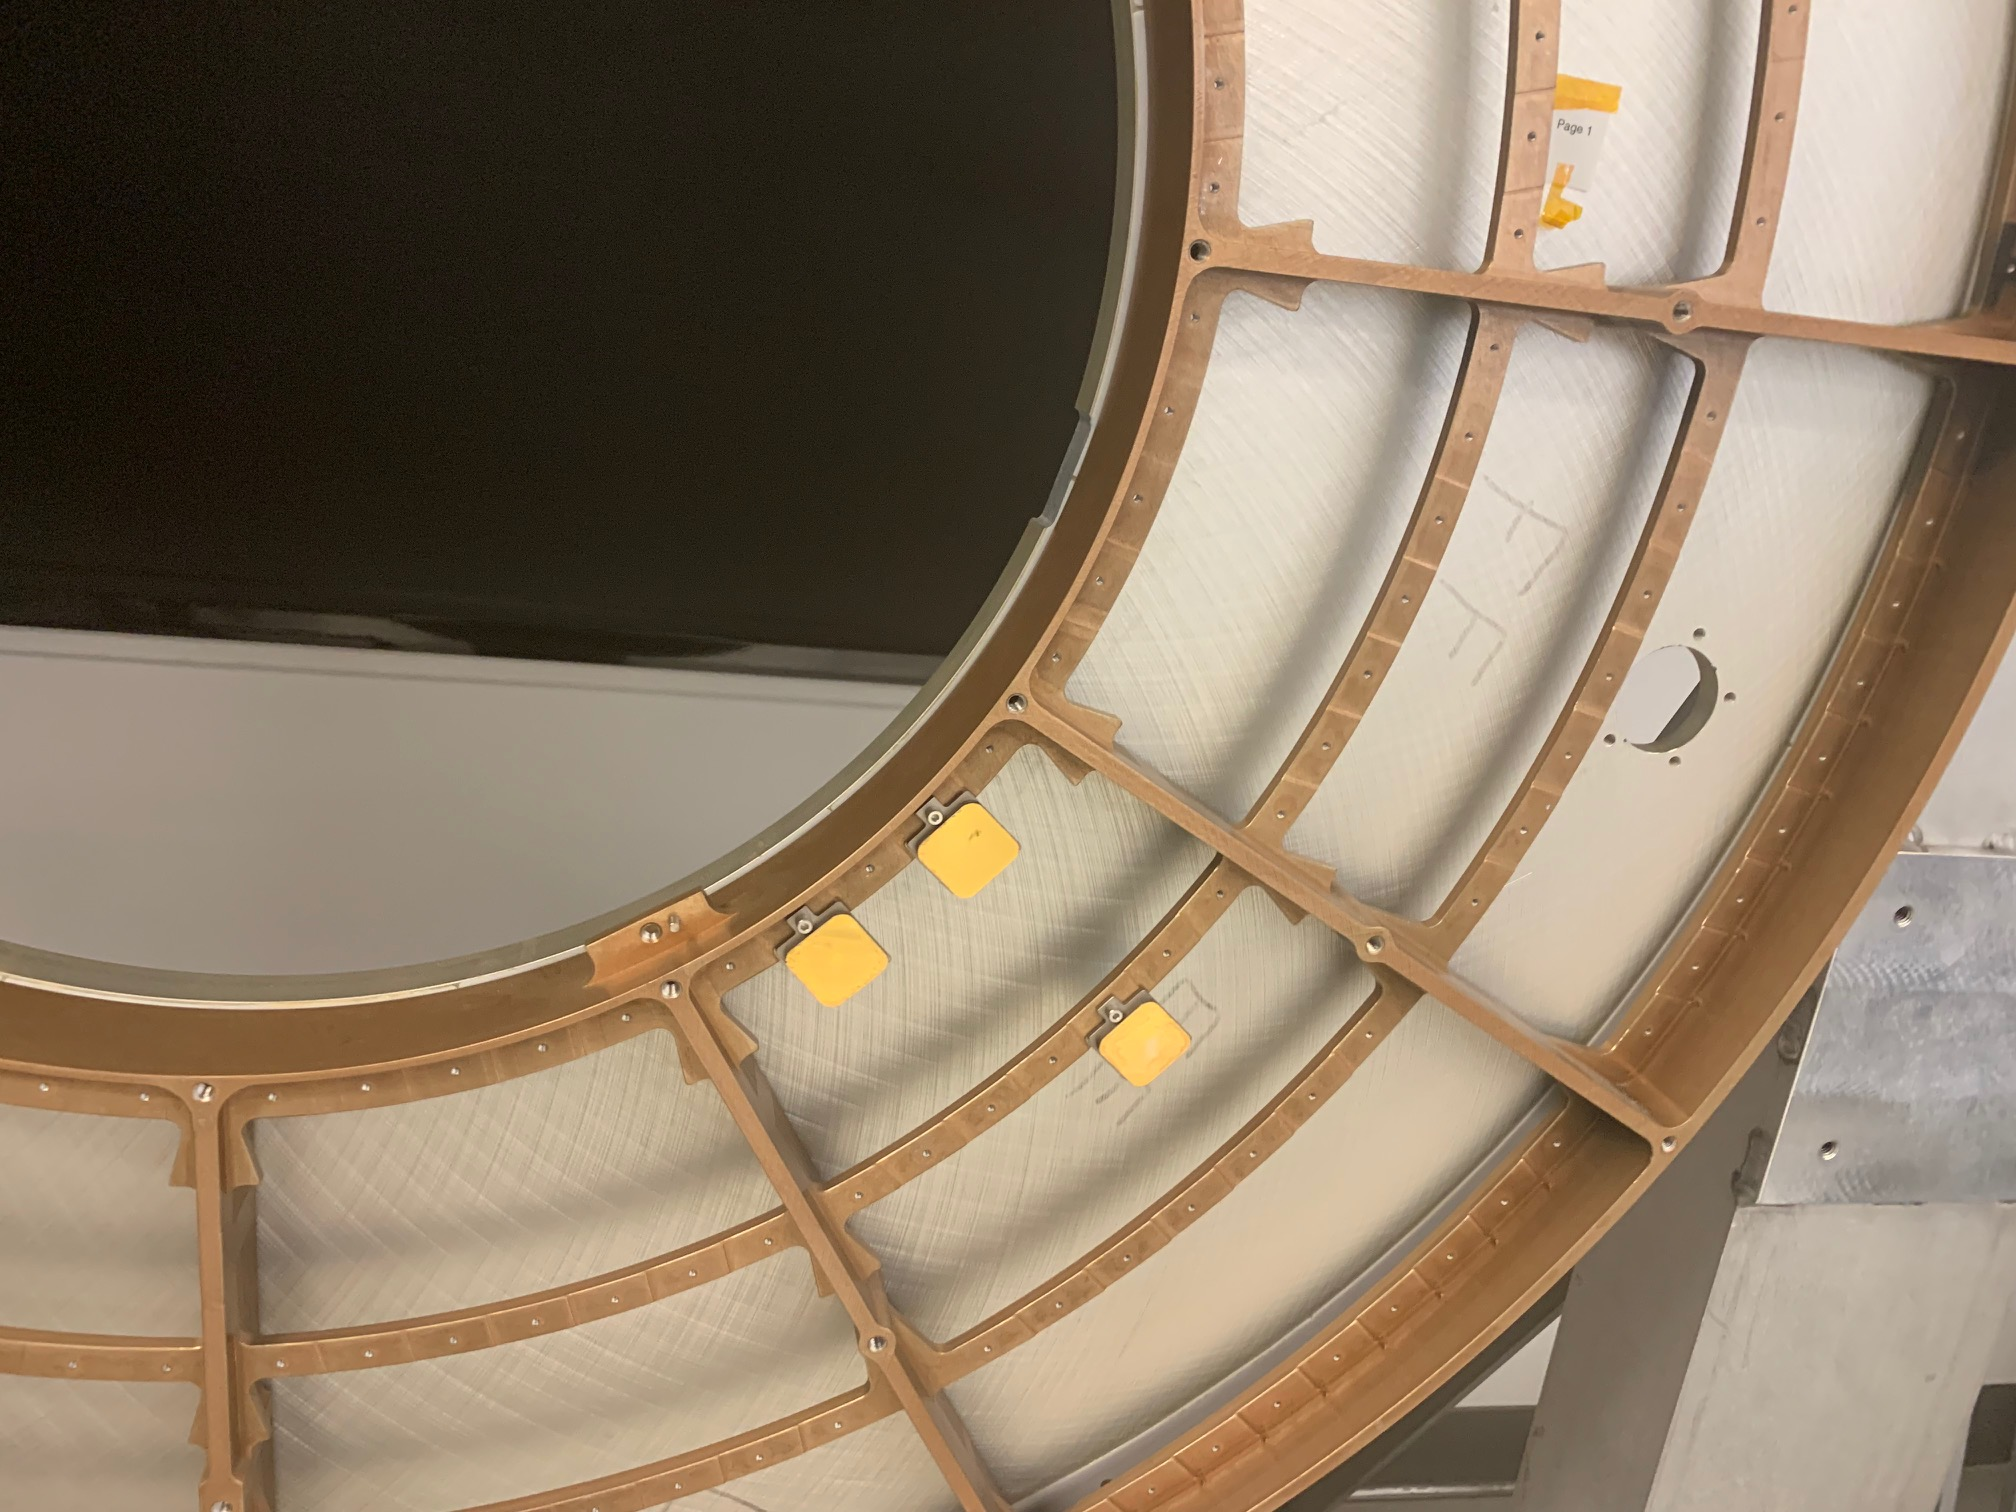
\includegraphics[width = 0.6\linewidth]{Chapters/Figures/facet.jpg}
    \caption{A portion of a life-size model of the HESS at MIT/CXC showing three HEG grating facets and the support frames (image taken by the author of this thesis).}
    \label{facet}
\end{figure}




\section{High resolution X-ray spectral Analysis}
\subsection{Data Preparation}

\subsubsection{Detecting X-rays with Chandra}
The ACIS detector consists of CCDs chips that can record not only the positions of the photons on the detector, but also the photon's energy and time of arrival. However, there are instrumental issues that affect how photons of a given energy are redistributed into a number of ACIS detector channels. The formal description of the transformation from photons to counts is
\begin{equation}
    C(h) = T\int_0^{\infty}\sum_i R_i (E, h)A_i(E)S_i(E)dE + B(h),
\end{equation}

where 
\begin{itemize}
    \item $C(h)$ is the number of counts in detector channel $h$, \item $T$ is the exposure time,
    \item $R_i(E,h)$ is the detector redistribution from energy E to channel $h$ (This information is encoded in Response Matrix File, or RMF, that is generated for every observation) for the source component $i$,
    \item  $A_i(E)$ is the effective area (geometric area $\times$ filter efficiency $\times$ detector quantum efficiency)(This information is encoded in Ancillary Response File, or ARF, that is also generated for every observation) at energy E for source component $i$,
    \item $S_i(E)$ is the source photon flux at energy E for component $i$,
    \item $B(h)$ is the background counts in channel $h$. This could include both cosmic and internal sources, empirical or modeled, possibly from other observations \citep{Huenemoerder_lec_2011}.
\end{itemize} 

The basic data product from which all analysis follows is the \textit{event list} provided as a Flexible Image Transport System (FITS) binary table, which includes information such as time, detector element ID, detector X pixel, detector Y pixel, pulse height amplitude (PHA), etc \citep{Huenemoerder_lec_2011}.\par


% An HETGS count spectrum produced by standard analysis (a PHA file) can be related to the source spectrum through a grating ARF (Auxiliary Response File) and grating RMF (Redistribution Matrix File).\par 

The ARF contains the effective area as a function of energy for an observation \citep{Huenemoerder_lec_2011}. When a physical spectrum is multiplied by an ARF, the result would be the distribution of counts that received by a detector. The ARF includes the efficiencies of mirrors, gratings, filters and detector.  Figure~\ref{effective} shows an example of effective area vs. energy graph. Edges in the graph are due to different non-uniformities.


\begin{figure}[ht!]
\centering
  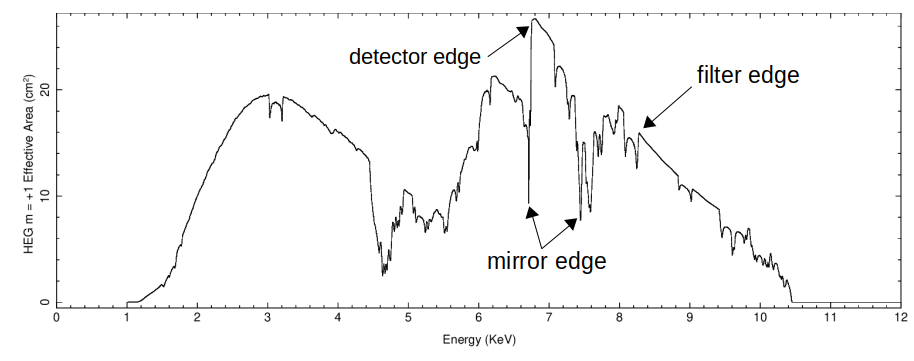
\includegraphics[width = \linewidth]{Chapters/Figures/effective_area_label.png}
  \caption{The HETGS HEG +1 effective area from an ARF file of 2018 Chandra observation. Edges of detector, mirror and filter are labeled in the graph.}
  \label{effective}
\end{figure}


An RMF is a standardized format FITS file that encodes the relationship between the incident photon energy and the output signal's distribution over channels (such as detector pulse heights or PHA).  High energy photons encounter detector and interact with the detector material (e.g., silicon for CCDs). When a photon is absorbed in the silicon of a CCD, a charge cloud of electron-hole pairs is formed ($\approx$ 3.65 eV per pair)\citep{Davis2008}. PHA is a measure of the number of pairs in the cloud. The response matrix accounts for how the
detector redistributes photons of a given
energy. Figure~\ref{rmf} shows the visualization of the RMF of the ACIS-S3 chip. For photons of energy E, there is a probability distribution that describes how many counts can be expected in each detector channel. As incoming photon energy increases, the peak of the distribution shifts to greater
pulse height amplitudes, or detector
channel. When modeling a Chandra X-ray spectrum, the source model must first be multiplied by the effective area curve. Then the result is multiplied by the response matrix that redistributes modeled photon flux into detector channels. The final result is a model X-ray spectrum of counts vs. pulse height amplitude, which can be compared to the observed X-ray spectrum \citep{Doe2009}.

\begin{figure}[ht!]
    \centering
    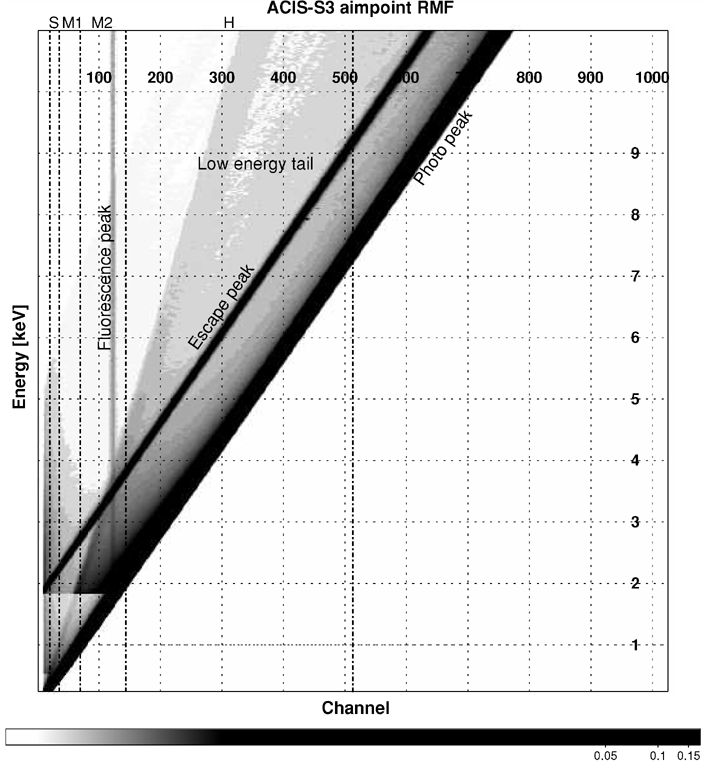
\includegraphics[width = 0.7\linewidth]{Chapters/Figures/rmf.png}
    \caption{Response matrices ACIS-S3 at the aim point. Grayscale is logarithmic. Numbers on the right-hand side are energy in units of keV and numbers at the top are PHA/PI channel numbers. The vertical dash-dotted lines delimit the energy bands \citep{Grimm2009}.}
    \label{rmf}
\end{figure}


\subsubsection{Software and Data Analysis}

Prior to starting HETG data analysis, few software packages need to be downloaded and installed. ISIS \citep{Houck2000} denotes the Interactive Spectral Interpretation System, which supports the analysis of high resolution X-ray spectra using the database of atomic data and plasma emission models. CIAO tool \citep{CIAO2006} is the software package developed by the Chandra X-Ray Center for analyzing data from the Chandra X-ray Telescope. TGCAT denotes The Chandra Transmission Gratings Archive and Catalog, which makes grating spectra easily viewable and analyzable \citep{Huenemoerder2011}. Data processing for the TGCAT catalog is done with a collection of ISIS/S-Lang scripts. TGCAT uses both CIAO and ISIS\par

The first step is to download observations from the online Chandra data archive and configure the data directories to optimize our processing requirements. Then we set the ISIS and CIAO environment so that necessary tools are in the path. We then use TGCAT to extract the PHA, ARF, RMF, as well as the summary plots. The detailed files generated are as follows. 
\begin{itemize}
    \item \textbf{evt0.par} An ASCII file listing header keywords and values from the event file.
    \item \textbf{evt1} The level 1 event file that contains all the events recorded for the observation.
    \item \textbf{evt2} The level 2 event file created by the level 1 event file. A FITS binary table, containing the grating coordinates, time, and other information for each good event. 
    \item \textbf{\*\_\#.arf} ``Ancillary Response Files'' for different gratings. \# is a diffraction order, either -1 or 1. 
    \item \textbf{\*\_\#.rmf} ``Response Matrix Files'' for different gratings. \# is a diffraction order, either -1 or 1. 
    \item \textbf{pha2\*} ``Pulse Height Amplitude'' files for binned spectrum and binned background
    \item \textbf{summary\_flux\_overview.ps} Overview flux spectrum plot
    \item \textbf{summary\_fprops.fits} Flux properties (FITS binary table). Contains counts and rates summed in bands. For coarse characterization. 
    \item \textbf{summary\_[hm]eg}  Order sorting image (FITS image), for all photons.
    \item \textbf{summary\_[hm]eg\_all.fits (H)} Order sorting image (FITS image), for filtered, binned photons. 
    \item \textbf{summary\_im-a.ps} Summary image; source region detail (Figure~\ref{xpattern})
    \item \textbf{summary\_im-b.ps} Summary image; sky field image (Figure~\ref{skyfield}).
    \item \textbf{summary\_imsp.ps} Summary image; spectral-spatial image 
    \item \textbf{summary\_lc.ps } Summary plot; light curve 
    \item \textbf{summary\_spc.ps } Summary plot; counts (Figure~\ref{spc})
    \item \textbf{summary\_spf.ps} Summary plot; flux (Figure~\ref{spf})
\end{itemize}

\begin{figure}[ht!]
    \centering
    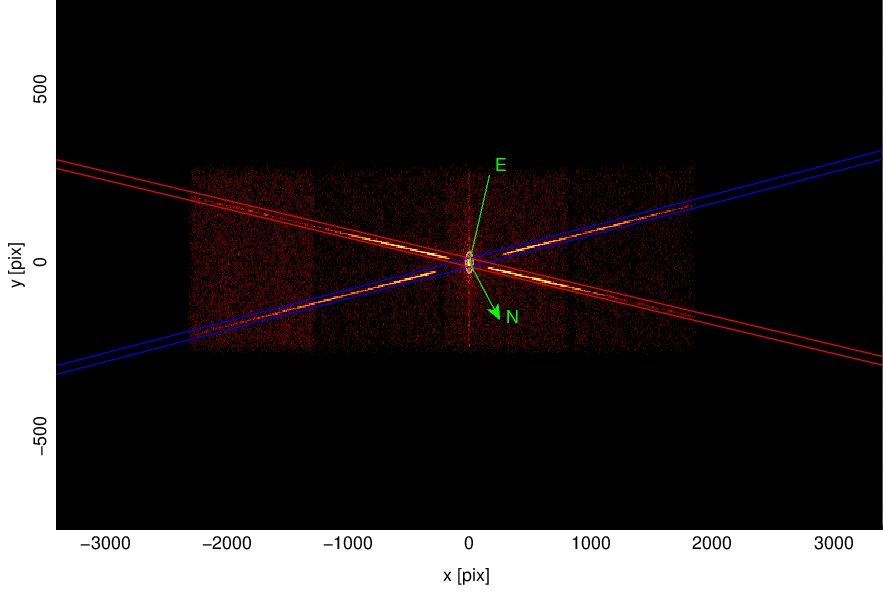
\includegraphics[width = \linewidth]{Chapters/Figures/sky_field.png}
    \caption{An ``X'' pattern of the spectrum. The blue line shows the high energy spectrum and the red line shows the medium energy spectrum.}
    \label{skyfield}
\end{figure}

\begin{figure}[ht!]
    \begin{minipage}[t]{0.45\textwidth}
        \centering
        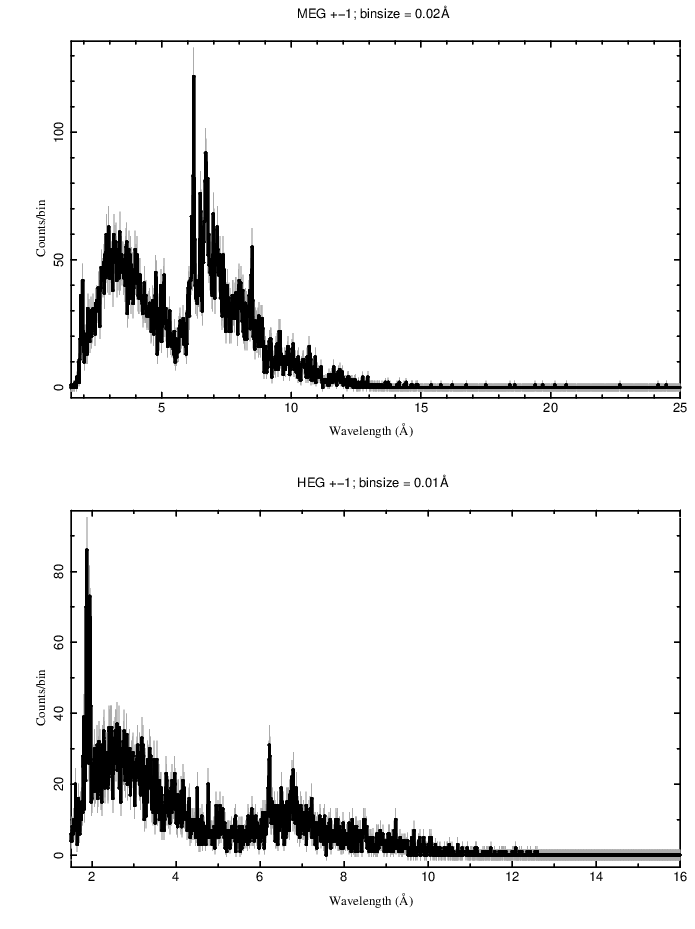
\includegraphics[scale = 0.3]{Chapters/Figures/spc.png}
        \caption{Counts vs. wavelength spectral plot.}
        \label{spc}
    \end{minipage}
    \begin{minipage}[t]{0.6\textwidth}
        \centering
        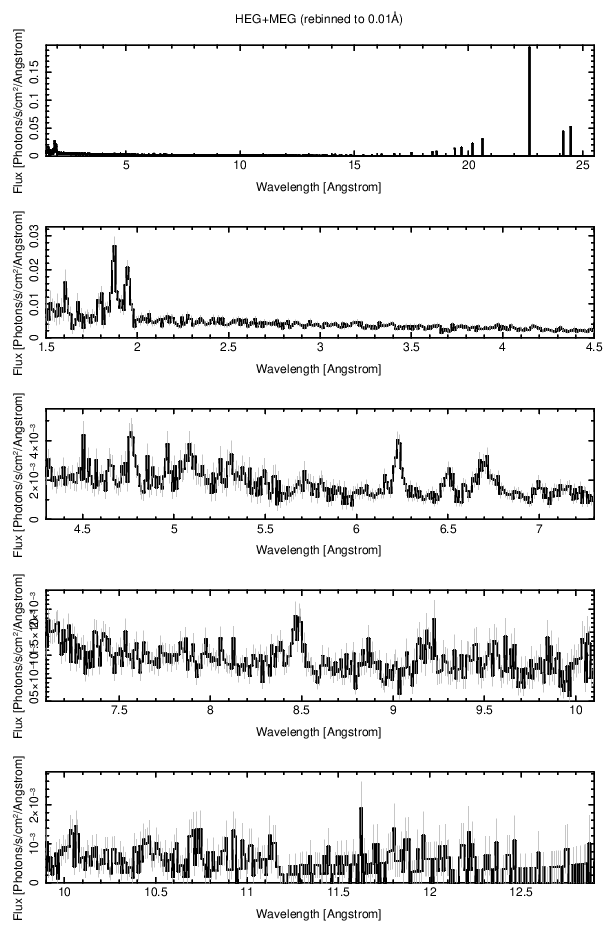
\includegraphics[scale = 0.35]{Chapters/Figures/spf.png}
        \caption{Flux vs. wavelength spectral plot.}
        \label{spf}
    \end{minipage}
\end{figure}




\subsection{Choosing the Right Fit Statistic}
Parameter estimation performed in ISIS finds the parameters for a given model that fit the data best. Statistics estimates the uncertainties on these parameters and tests whether model's best-fit parameters match with the data. \citep{Arnaud1999}. \par 
Which statistics to use depends on the probability distributions underlying the data. Almost all astronomical data are drawn from one of two distributions: Gaussian or Poisson \citep{Arnaud1999}. Poisson distribution is valid if the only source of the experimental noise is due to the number of events arriving at the detector, for example, modern CCD instruments \citep{Arnaud1999}. If some other sorts of noise is significant then it could be described by the Gaussian distribution. One common example would be background needs to be modeled in some way, rather than directly measured. The uncertainty in the background modelling is assumed to be Gaussian \citep{Arnaud1999}. \par

In order to assess the validity of models, hypothesis test can be formulated about astrophysical process. A well-known test is based on Pearson’s $\chi^2$ statistic
\begin{equation}
    S \equiv \sum_{i = 1}^{N}\dfrac{(D_i - F_i)^2}{\sigma^2}
    \label{chi}
\end{equation}
where $D_i$ is the number of observed counts in bin $i$, $F_i$ are the number of counts predicted by the model and $\sigma_i^2 = F_i$ is the deviations which are approximately Gaussian \citep{Lampton1976}. 

It is easier to obtain the best-fit parameters of the model by minimizing $\chi^2$ when $\sigma_i^2$ is approximated by a large source intensity. However, X-ray spectra of astrophysical sources are often characterized by relatively low amounts of counts per spectral bin.  Chi-squared test doesn't work well when there are low numbers of counts per spectral bin \citep{Kaastra2017}. From Equation~\ref{chi}, we can see that it fails for small source intensity by putting $\sigma_i$ = 0 in the equation.\par 
Another method found by Webster Cash solved this problem \citep{Cash1979}. The discrete Poisson distribution:
\begin{equation}
    \text{prob}(D_i) = p(D_i|M_i) = \dfrac{M_i^{D_i}}{D_i!}e^{-M_i}
    \label{poisson}
\end{equation}
which represents the probability of finding $D_i$ event (counts) in bin $i$ (energy range) of data set D (spectrum) in a given length of time (exposure time), if the events occur independently at a constant rate $M_i$ (source intensity) \citep{Siemiginowska09}.\par 

In order to find the best parameter $M_i$ to fit the model the data better, it is natural to maximize the product of Poisson probabilities in each data bin $i$, i.e., to maximize the Poisson likelihood.

\begin{equation}
    L = \prod_i^{N} \dfrac{M_i^{D_i}}{D_i!}e^{-M_i} =\prod_i^{N} p(D_i|M_i)
    \label{maxhood}
\end{equation}

In practice, what is often maximized is the -2 log-likelyhood. After taking -2log of Equation~\ref{maxhood}, it becomes 
\begin{equation}
    C = 2\sum_i^{N} (M_i - D_i\mathrm{log}M_i) \propto -2L
    \label{cash}
\end{equation}
This is a well known statistic in X-ray astronomy which is called ``Cash Statistic''.\par 
 
 
 
 
 
 
 
 
 
 
 
 
 
 
 
 
 
 
 
%  The goodness of fit is expressed as 
% \begin{equation}
%     \chi^2 = \displaystyle\sum_{i=1}^n \dfrac{(M_i - s_i)^2}{\sigma_i^2}
%     \label{chisq}
% \end{equation}
% where the summation over i is over all n bins of the spectrum, $M_i$ is the observed number of counts, $s_i$ is the expected number of counts for the tested model, and $\sigma_i^2 = s_i$ for Poissonian statistics \citep{} \par 

%  Also, considering the data in a bin is downward fluctuation. Since we estimate the variance (in the denominator) using the observed data, the downward fluctuation contributes more to chi-squared than an upward fluctuation, resulting the biased best-fit model \citep{arnaud2012}. Therefore, it is not a proper method for spectrum that has small amount of counts per bin. Although there are methods to improve this problem, drawbacks still exist. For example, \cite{Gehrels1986} approximation for $M_i$ causes problems when the spectra are rebinned \citep{Kaastra2017}. \par 
% It was found out by \cite{Cash1979} that 
% \begin{equation}
%     \Tilde{C} = 2\displaystyle\sum_{i = 1}^n s_i - M_i\ln{(s_i)}
%     \label{cash}
% \end{equation}
% is a better statistics and can be applied to bins with a small number of counts. In Equation~\ref{cash}, $M_i$ is not in the denominator, so we do not need to worry about problems caused by upward or downward fluctuations.\par 






 








%\end{document}
  \chapter{Phenomenological modeling of our HETGs data}
\section{Introduction to Our Observation}
During 2018 August 10-14, SS 433 was observed using the High Energy Transmission Grating Spectrometer System (HETGS) on the Chandra X-ray Observatory. The full observing plan consisted of two parts. The first part is a 20 ksec observation, which was taken 3 days before the accretor was completely blocked by the donor (an eclipse) (See Figure~\ref{video_short} for the geometry). The orbital phase of the starting of the observation was 0.802. The second part was a 96 ksec long observation, which started right at the middle of the eclipse (See Figure~\ref{video_long1} and \ref{video_long2} for the geometry). The purpose of this observation was to use the eclipse of the accretor by the donor to map out the spatial variation of the jet's properties such as temperature, density ionization state, bulk jet-speed, composition, etc. We hoped to achieve our objective by comparing and analyzing spectra from two observations. In this chapter, we describe spectral fitting with phenomenological models, using line-grouping method and the blind search method. \par 


\begin{figure}
    \centering
    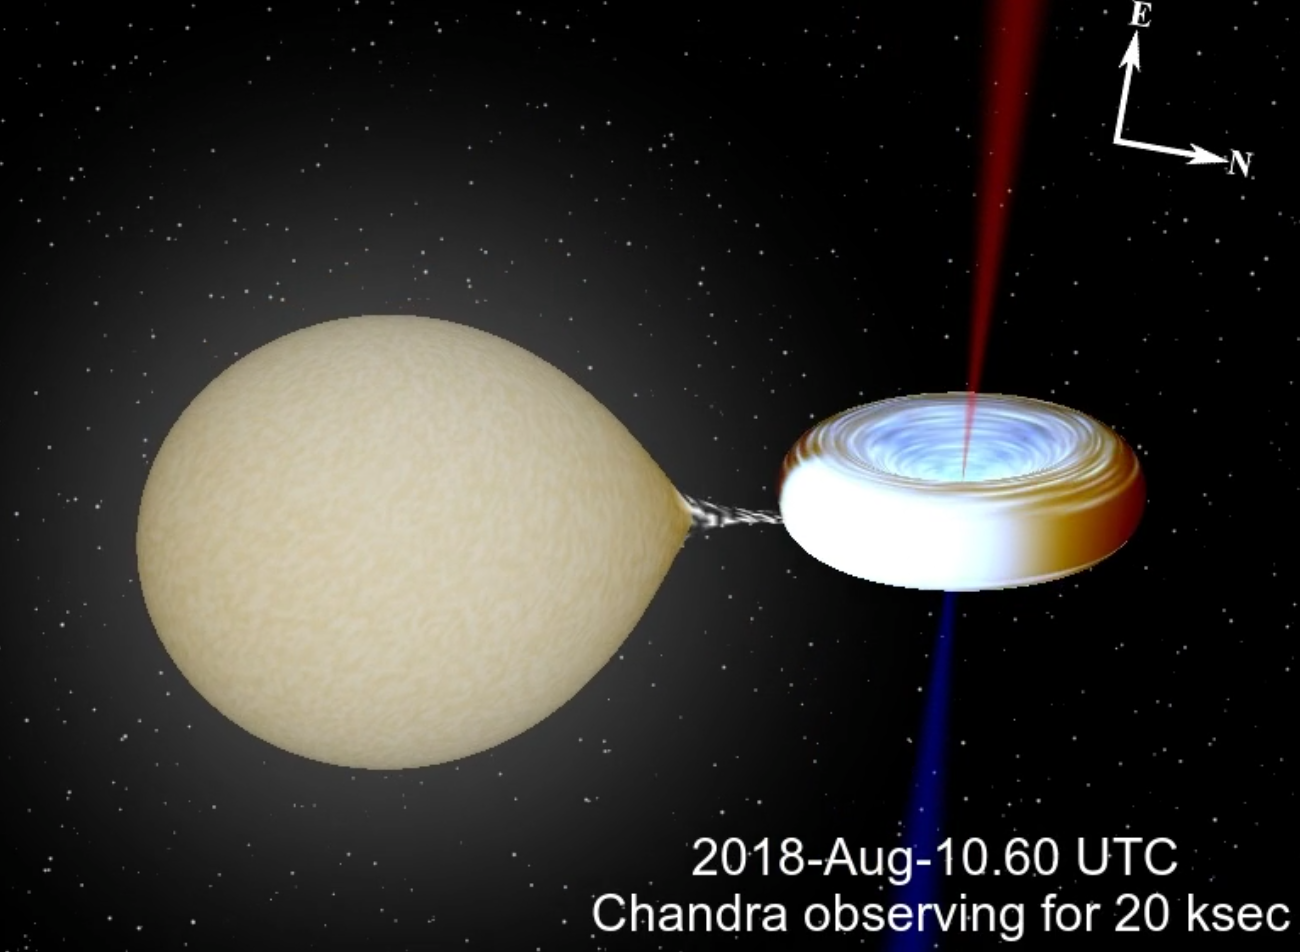
\includegraphics[scale = 0.2]{Chapters/Figures/video_short.png}
    \caption{The geometry of the starting time of the 20 ksec observation.}
    \label{video_short}
\end{figure}

\begin{figure}[h!]
    \centering
    \begin{subfigure}[t]{.4\textwidth}
        \centering
        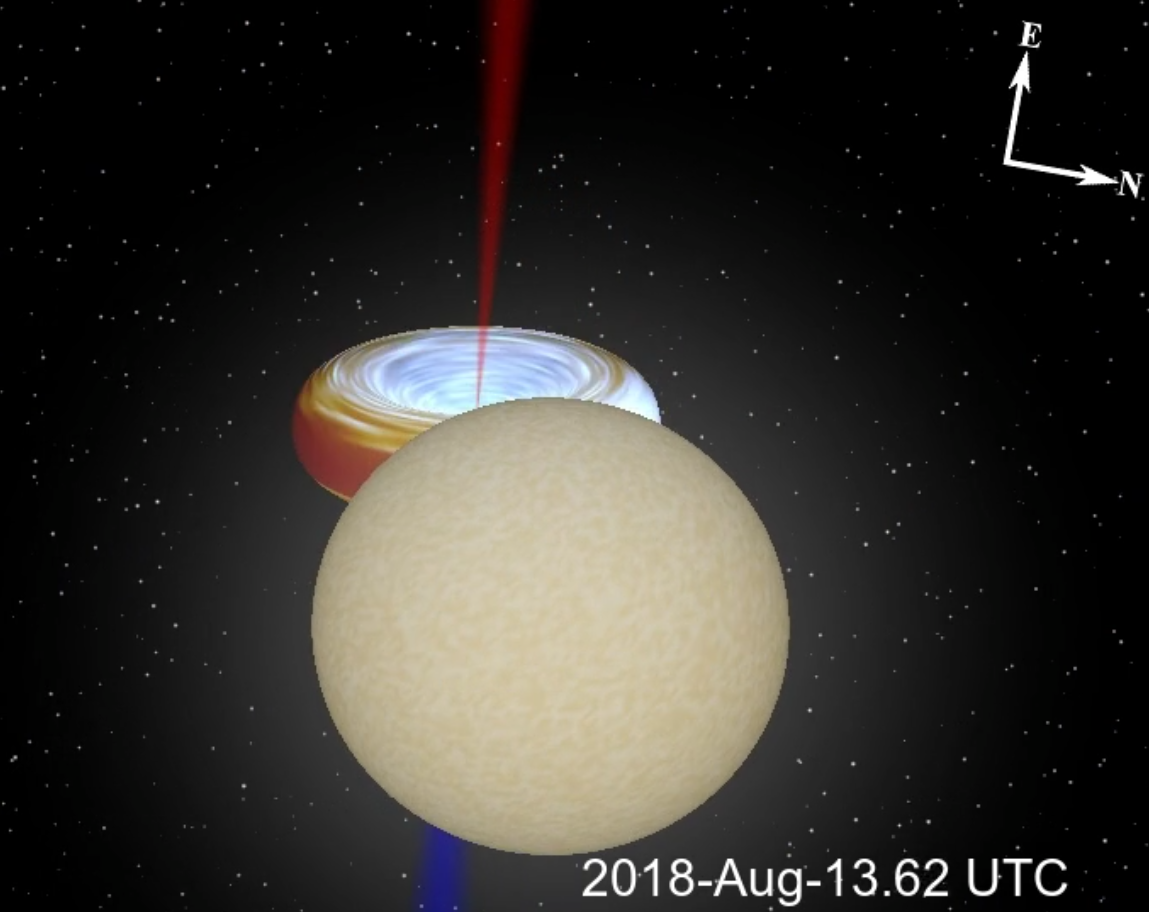
\includegraphics[width=0.94\linewidth]{Chapters/Figures/video_long.png}
        \caption{The geometry of the starting point of the 96 ksec observation.}
        \label{video_long1}
    \end{subfigure}%
    \hspace*{4em}
    \begin{subfigure}[t]{.4\textwidth}
        \centering
        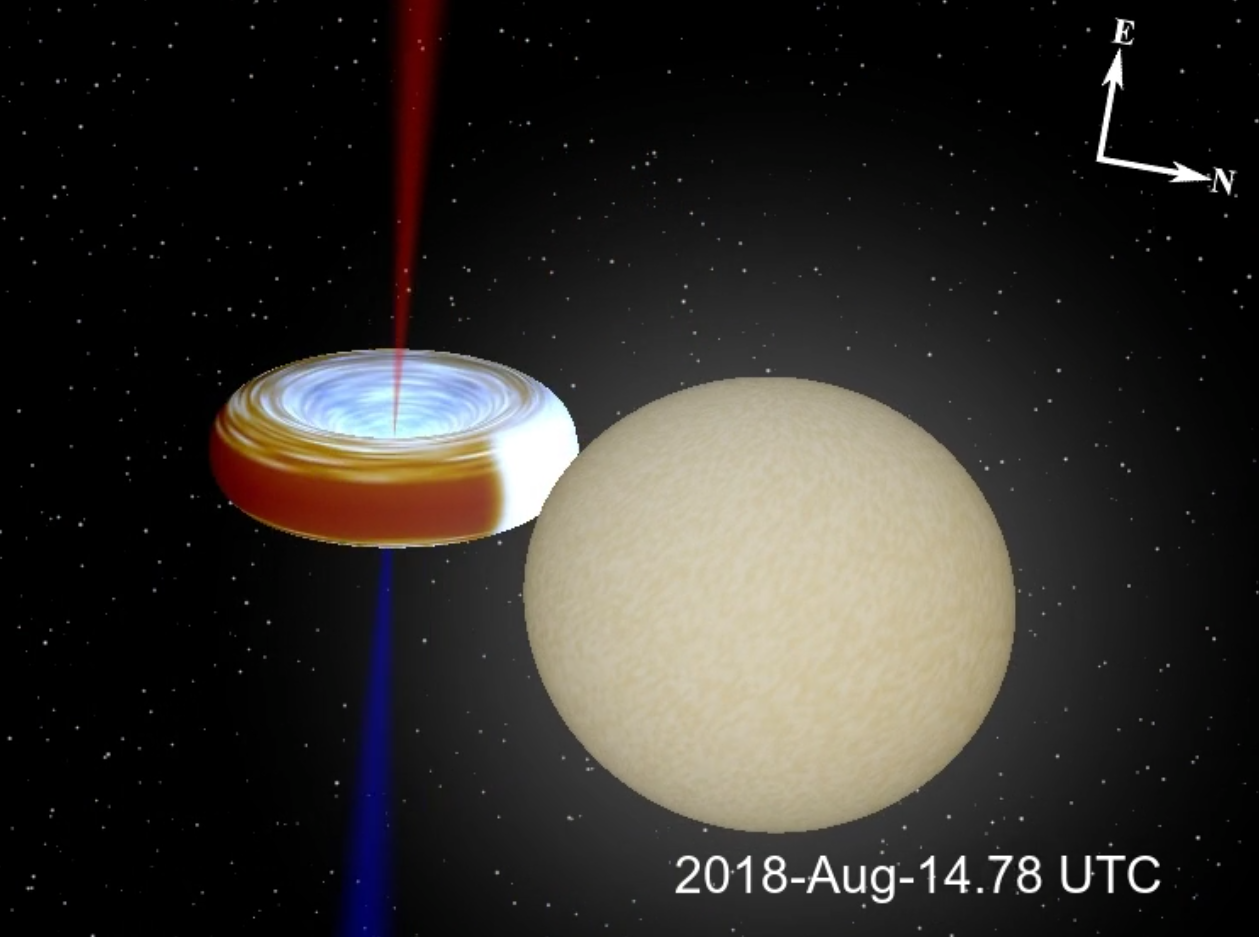
\includegraphics[width=\linewidth]{Chapters/Figures/video_long2.png}
        \caption{The geometry of the ending point of the 96 ksec observation.}
        \label{video_long2}
    \end{subfigure}
    \label{video_long}
\end{figure}




\section{The 20 ksec Observation on August 10, 2018}
\subsection{Method}
The emission lines on the spectra usually tell the most about the properties of the jets. The summary plots produced by TGCAT \citep{Huenemoerder2011} give a general idea of where the emission lines are (see Figure~\ref{summaryplot_el}). Previous papers \citep{Marshall2002, Marshall2013, Lopez2006} show the corresponding rest wavelengths of normal emission lines from those heavy elements. There are also other ways to access the accurate emission line wavelengths database. The X-Ray Data Booklet \citep{thompson2001} shows a complete energies of X-ray emission lines. The corresponding wavelengths can be found by 
\begin{equation}
    E = hc/\lambda.
\end{equation}


\begin{figure}
    \centering
    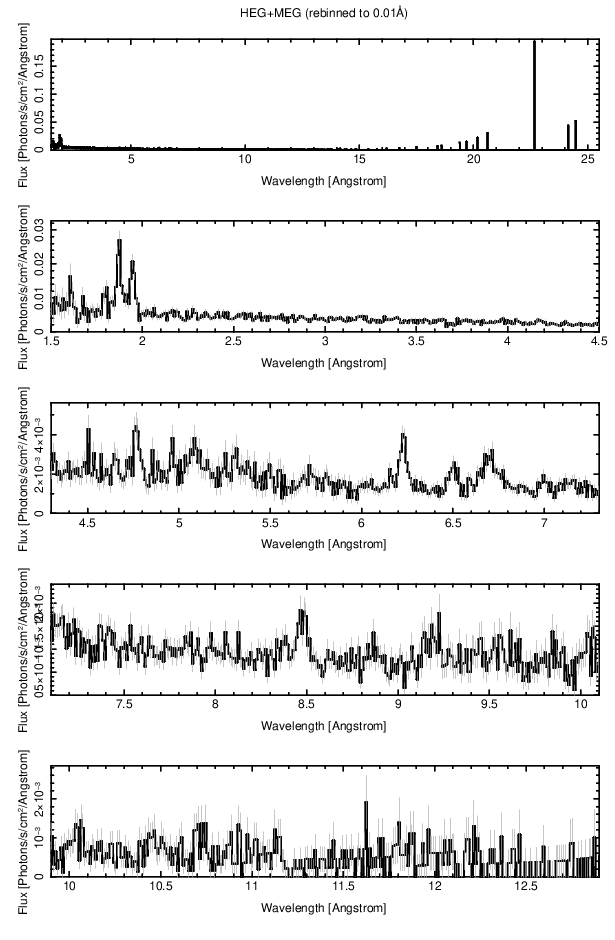
\includegraphics[width = 0.7\linewidth]{Chapters/Figures/summaryplot_el.png}
    \caption{A summary plot of 2018-08-10 Chandra observation produced by TGCAT \citep{Huenemoerder2011}. The plot shows the line fluxes over wavelength. }
    \label{summaryplot_el}
\end{figure}

Phenomenological models (models that describe the observed data, but are not directly derived from any physically motivated theory) are built to fit the continuum spectrum and the emission lines so that the line fluxes as well as the continuum's properties can be measured and studied. \par 
%This model determines the best redshift value of a jet by fitting all observed emission lines from one jet based on its rest wavelength and the redshift of the jet. 

After generating the PHA file and the corresponding ARF and RMF files, using a script written in ISIS to fit the group-line model to the spectrum. The script initially loads the APED so that theoretical wavelengths, radiative transition rates, and electron collisional excitation rate coefficients for most known X-ray transitions can be accessed. \par 
To simplify the fitting process, we start by fitting a few line profiles to a small part of the spectrum. Therefore, it is important to initially ignore all other spectra and all bins outside the region of interest. \par 
Usually one does not want to use the full resolution of a spectrum, either because the channels oversample the spectral resolution or because the signal-to-noise ratio for each bin is low. It is effective to assign the values to groups, to create a smaller set of discrete ranges. For our data, we grouped every 4 PHA channels in the MEG (or the HEG) together. Then we ignored a certain range of HEG and MEG data due to lack of good calibration data in these range. After excluding these energies, we used 1.25 - 10 \AA\ range of HEG data and 2.5 - 13 \AA\ range of MEG data. \par 


Since we know the orbital period and the precession period of the binary, we computed the predicted redshift values for both red and blue jets with a C program based on the kinematic model \citep{Margon1979}. Given the MJD (Modified Julian Date: number of days after midnight on November 17, 1858) of the observation, the program computes the corresponding predicted redshifts for both Western and Eastern jets at certain times. For the precession phase of our 20 ksec observation, the predicted blue- and red-shifts were 0.009234 and 0.06791 for the Western and Eastern jet, respectively. \par

\subsubsection{Line-grouped Model}
One of the models used here is called the line-grouped model. Precise redshift for these emission line profiles were determined by fitting lines from the same jet together with several Gaussian components of known rest wavelength values taken from Astrophysical Plasma Emission Database (APED) \citep{smith2001}.\par
We define a fit function which is a combination of multiplicative models and additive models. \textbf{wabs} is a multiplicative model that describes photoelectric absorption due to neutral gas between us and SS 433 \citep{Arnaud1999}. It modifies the observed spectrum so that the spectrum has a proper continuum. In the additive model, there are two main components. The first one is a power law, fitting the continuum spectrum 
\begin{equation}
     N(E) = KE^{-\alpha},
     \label{powerlaweq}
\end{equation}
where $K$ is photons/keV/cm$^2$/s at 1 keV and $\alpha$ is the photon index. The second one is the sum of many Gaussian distributions
\begin{equation}
     N(E) = K\dfrac{1}{\sigma \sqrt{2\pi}}\mathrm{exp}(\dfrac{-(E-E_l)^2}{2\sigma^2}, 
\end{equation}
where $K$ is the total photons/cm$^{-2}$/s in the line, $E_l$ is line energy in keV and $\sigma$ is line width in keV. Each emission line profile is modeled using one Gaussian.\par 

After defining the fitting function, we set the parameter values. The parameters include the starting best-guess values of two redshifts (one for each jet), two error terms for the redshifts, the rest wavelengths of all the elements, Gaussian widths and Gaussian areas. Since there are many parameters to fit, we give a physically plausible search range for each of the parameter, thereby speeding up the convergence of the fitting. \par 

Cash statistic was applied to find the best model fit to the data, which means the least model deviation from the data. Lines were fitted to the MEG and HEG data separately in their own wavelength ranges. Precise redshifts of both jets for these profiles were determined by fitting the emission lines of known rest wavelength values.\par


\subsubsection{Blind Fitting Method}

To determine the wavelengths and fluxes of the observed emission lines and their errors, we used a blind fitting method to fit the spectra. In this method, Voigt function, similar to Gaussian, is used to fit the emission lines. The Voigt profile is the convolution of the natural resonance of an emitted line with the Maxwellian speed distribution \citep{Houck2000}. The natural resonance profile is a Lorentzian with full-width at half maximum, $\Gamma/4\pi$. The Maxwellian speed distribution is a Gaussian with velocity width $v_o = \left(\dfrac{2kT}{m}\right)^{1/2}$, where $m$ is the ion mass and $T$ is the temperature. Unlike the previous fitting method, this fitting model does not depend on redshift. By indicating the center of an emission line, the model is fit to the spectra.

\subsection{Results}

The spectra are shown in Figure~\ref{shorthegpheno} - Figure~\ref{shortmegpheno}. Similar to previous observations, typical emission lines of irons, nickel, sulfur, and silicon and a significant continuum are prevalent. Emission lines from the Western and Eastern jets are prominent enough to find the  accurate measurement of redshifts for both jets. \par

\begin{figure}[h!]
    \centering
    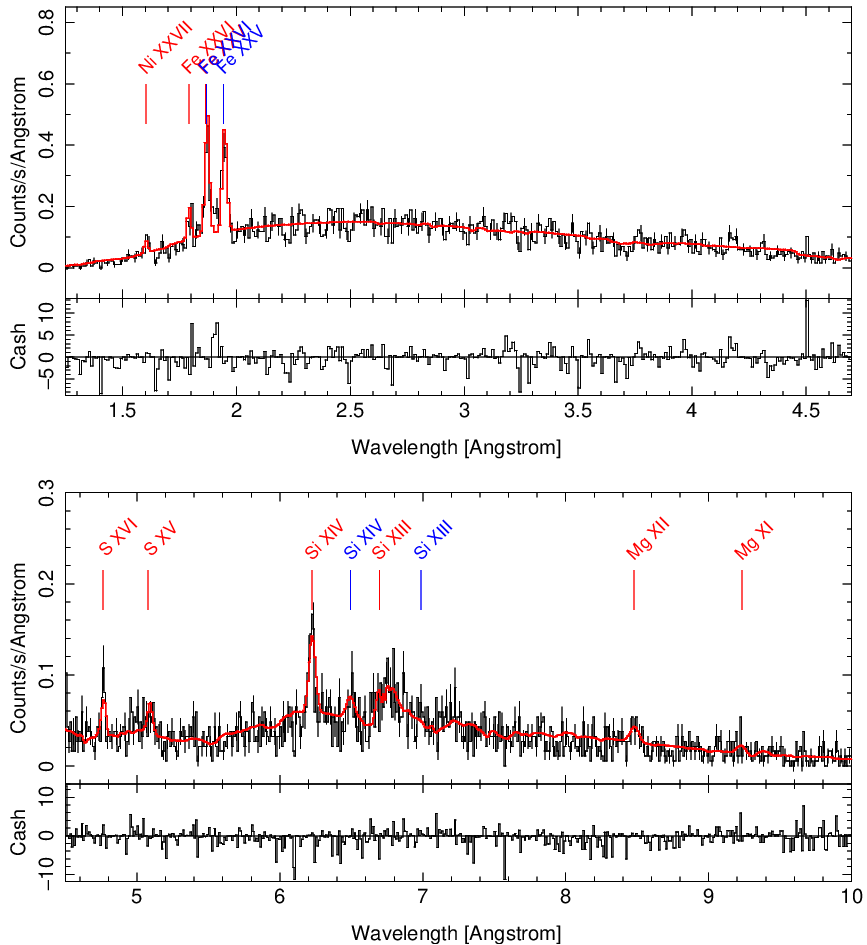
\includegraphics[width = \linewidth]{Chapters/Figures/short_pheno_heg.png}
    \caption{The 20 ksec X-ray spectrum of SS 433 observed with the Chandra HETGS on 2018-08-10. This set of figures show the spectrum from the HEG data. The Bremsstrahlung radiation likely creates the continuum. Red line: phenomenological model fit to the spectrum from 1.25\AA -  10\AA. Line identifications are labeled where there are features in the spectrum and confirmed by the model. The red characters label the emission lines from the Western jet while the blue ones from the Eastern jet. The Cash statistic residuals are shown at the bottom of each spectrum. }
    \label{shorthegpheno}
\end{figure}



\begin{figure}[h!]
    \centering
    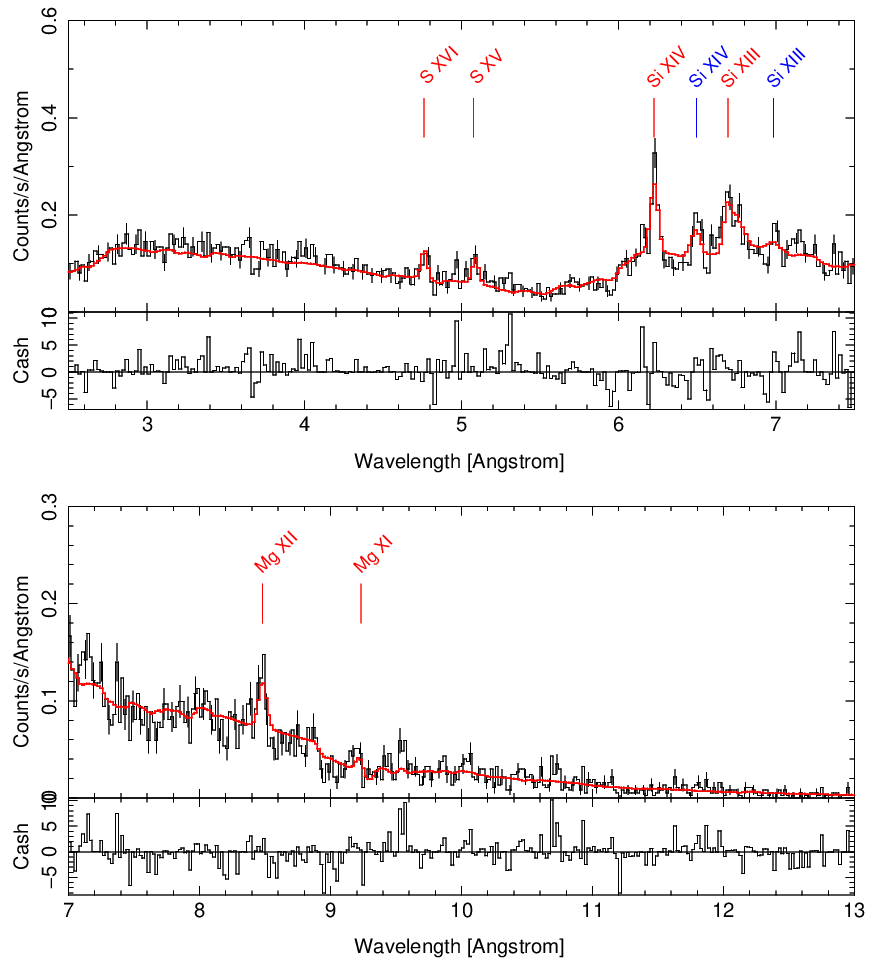
\includegraphics[width = \linewidth]{Chapters/Figures/short_pheno_meg.png}
    \caption{Same as Figure~\ref{shorthegpheno} but showing the X-ray spectrum of SS 433 from the MEG data. Red line: phenomenological model fit to the spectrum from 2.5\AA -  13\AA.}
    \label{shortmegpheno}
\end{figure}

\newpage
\newpage
\newpage
The line fluxes are shown in Table~\ref{tab:shortlinefluxes_west} - \ref{tab:shortlinefluxes_east}.  $z$ denotes the redshift. There are more detectable lines from the Western jet than the Eastern jet as predicted since our observation was taken when the Western jet is approaching while the Eastern jet is receding. The Eastern jet will be somewhat fainter than the Western jet, when there was a large difference in the Eastern and Western Doppler shifts. \par 




\begin{deluxetable}{lccccr}
\tablecolumns{5}
\tablewidth{0pc}
\tabletypesize{\small}
\tablecaption{SS 433 Western Jet Line Diagnostics Using Voigt profiles for the 20 ksec Observation
\label{tab:shortlinefluxes_west}\tablenotemark{a} }
\tablehead{\colhead{Identification}& \colhead{$\lambda_{\rm rest}$} & \colhead{$\lambda_{\rm obs}$} & \colhead{$z$}
    & \colhead{Line Flux}  & \colhead{$\sigma$} \\
  \colhead{}& \colhead{(\AA)} & \colhead{(\AA)} & \colhead{}
    & \colhead{($10^{-6}$ ph \mathrm{cm$^{-2}$ s$^{-1}$})} & \colhead{\AA} }
\startdata
Ni{\sc xxvii}&	1.592&	1.608$\pm$	0.003&	0.0102$\pm$0.0018&	221.5$\pm$59.1&	0.0055\\
Fe{\sc xxvi}&	1.78&	1.798$\pm$	0.003&	0.0103$\pm$0.0014&	187.6$\pm$37.7&	0.0062\\
Fe{\sc xxv}&	1.855&	1.875$\pm$	0.001&	0.0107$\pm$0.0006&	459.1$\pm$49.5&	0.0064\\
S{\sc xvi}&	4.73&	4.767$\pm$	0.021&	0.0078$\pm$0.0044&	50$\pm$2&	0.0164\\
S{\sc xv}&	5.055&	5.084$\pm$	0.011&	0.0058$\pm$0.0021&	119.7$\pm$31&	0.0175\\
Si{\sc xiv}&	6.182&	6.227$\pm$	0.002&	0.0073$\pm$0.0003&	150$\pm$5.1&	0.0214\\
Si{\sc xiii}r&	6.648&	6.675$\pm$	0.005&	0.0041$\pm$0.0007&	59.9$\pm$10.4&	0.023\\
Si{\sc xiii}i&	6.687&	6.71$\pm$	0.004&	0.0035$\pm$0.0006&	78.3$\pm$12.1&	0.0232\\
Si{\sc xiii}f&	6.74&	6.761$\pm$	0.002&	0.0031$\pm$0.0003&	50.2$\pm$2&	0.0234\\
Mg{\sc xii}&	8.421&	8.472$\pm$	0.005&	0.0061$\pm$0.0005&	92.2$\pm$11.4&	0.0292\\
Mg{\sc xi}&	9.169&	9.188$\pm$	0.012&	0.002$\pm$0.0013&	86.2$\pm$15&	0.0318\\
\enddata
\tablenotetext{a}{All uncertainties refer to statistical 90\% confidence limits}
\end{deluxetable}


\begin{deluxetable}{rcccr}
\tablecolumns{5}
\tablewidth{0pc}
\tabletypesize{\small}
\tablecaption{SS 433 Eastern Jet Line Diagnostics Using  Voigt profiles for the 20 ksec Observation\tablenotemark{a}
\label{tab:shortlinefluxes_east} }
\tablehead{ \colhead{Identification}& \colhead{$\lambda_{\rm rest}$} & \colhead{$\lambda_{\rm obs}$} & \colhead{$z$}
    & \colhead{Line Flux}  & \colhead{$\sigma$} \\
   \colhead{} &\colhead{(\AA)} & \colhead{(\AA)} & \colhead{}
    & \colhead{($10^{-6}$ ph cm$^{-2}$ s$^{-1}$)} & \colhead{\AA}}
\startdata
Fe {\sc xxvi}& 1.78&	1.864 $\pm$ 0.002&	0.0471 $\pm$ 0.0011&	266.3 $\pm$ 48.2& 0.0087\\
Fe {\sc xxv} &1.855&	1.946 $\pm$ 0.0015&	0.0489 $\pm$ 0.0008&	500.3 $\pm$ 41.4 & 0.0084\\
Si {\sc xiv} &6.182&	6.501 $\pm$ 0.0036&	0.0516 $\pm$ 0.0006&	65.1 $\pm$ 9.9&	 0.0291\\
Si {\sc xiii}f & 6.74&	7.004 $\pm$ 0.0059&	0.0391 $\pm$ 0.0009&	37.5 $\pm$ 8.6& 0.0313\\
\enddata
\tablenotetext{a}{All uncertainties refer to statistical 90\% confidence limits}
\end{deluxetable}


%---------------------------------------------------
%--------------------------------------------------
%Long Observation
%---------------------------------------------------
%----------------------------------------------------------

\newpage
\section{The 95 ksec Observation on August 13 - 14, 2018}
Three days after the short observation, a 96 ksec long observation started almost in the middle of the eclipse. The orbital phase of the starting time was 0.0219 and the jet precession phase was 0.466 according to the kinematic model. In order to compare the change in spectral properties during the long observation, the total spectrum was split into 5 parts, each with 19.2 ksec. Same phenomenological model is fitted to the spectra of the five parts of long observation.  \par



\subsection{Results}
Figure~\ref{long_pheno0_heg} - \ref{long_pheno4_meg} in the Appendix shows the phenomenological fit with full wavelength for five parts. Figure~\ref{longportion} and \ref{shortportion} show that the Fe {\sc xxv} from the Eastern jet totally disappeared from the spectra when the long observation started. Figure~\ref{longportion2} and \ref{shortportion2} show that silicon lines from the Eastern jet appear fainter and the corresponding ones from the Western jet appear stronger in the first part of long observation comparing to the ones in the short observation. Since Fe {\sc xxvi} from the Eastern jet and Fe {\sc xxv} from the Western are blended, it is hard to tell whether the part of the Eastern jet showing Fe {\sc xxv} is also blocked by the companion star. At the end of the observation as shown in~\ref{long_pheno4_heg}, Fe {\sc xxv} from the Eastern jet did not show up, suggesting the part of the jet yielding Fe {\sc xxv} might had been still in the eclipse.\par


\begin{figure}[h!]
    \centering
    \begin{subfigure}[t]{.3\textwidth}
        \centering
        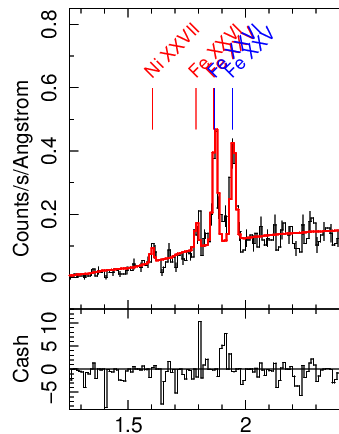
\includegraphics[width=\linewidth]{Chapters/Figures/short_pheno_part.png}
        \caption{1.25 - 2.4 \AA\ range of the Chandra HEG spectrum from the 20 ksec observation }
        \label{shortportion}
    \end{subfigure}%
    \hspace*{4em}
    \begin{subfigure}[t]{.3\textwidth}
        \centering
        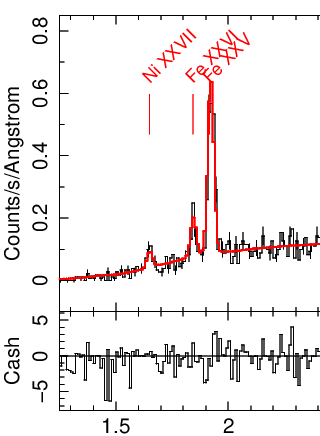
\includegraphics[width=\linewidth]{Chapters/Figures/long0_pheno_part.png}
        \caption{1.25 - 2.4 \AA\ range of the Chandra HEG spectrum from the first part of 96 ksec observation}
        \label{longportion}
    \end{subfigure}
    \label{portion}
\end{figure}


\begin{figure}[h!]
    \centering
    \begin{subfigure}[t]{.3\textwidth}
        \centering
        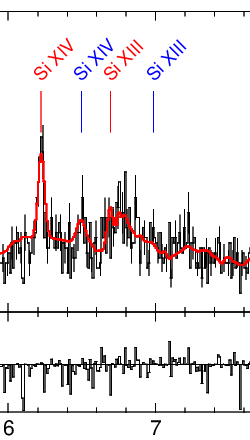
\includegraphics[width=\linewidth]{Chapters/Figures/short_pheno_part2.png}
        \caption{6-7.6 \AA\ range of the Chandra HEG spectrum from the 20 ksec observation }
        \label{shortportion2}
    \end{subfigure}%
    \hspace*{4em}
    \begin{subfigure}[t]{.3\textwidth}
        \centering
        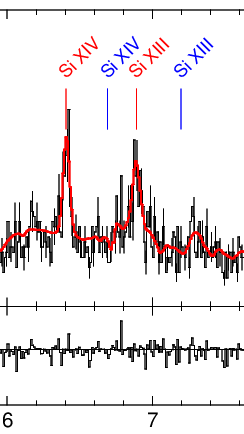
\includegraphics[width=\linewidth]{Chapters/Figures/long_pheno_part2.png}
        \caption{6-7.6 \AA\ range of the Chandra HEG spectrum from the first part of 96 ksec observation}
        \label{longportion2}
    \end{subfigure}
    \label{portion}
\end{figure}

\newpage
Applying the similar blind fitting method as the short observation, the line diagnostics for the long observation are shown in Table~\ref{tab:longlinefluxes_west} - \ref{tab:longlinefluxes_east}. With this model, Fe {\sc xxv} from the Western jet and Fe {\sc xxvi} from the Eastern jet could be fit with two Voigt profiles and thus line flux for each emission line was estimated.








\begin{deluxetable}{rccccr}
\tablecolumns{5}
\tablewidth{0pc}
\tabletypesize{\scriptsize}
\tablecaption{SS 433 Western Jet Line Diagnostics Using Voigt profiles for the 96 ksec Observation
\label{tab:longlinefluxes_west} }
\tablehead{\colhead{Identification}& \colhead{$\lambda_{\rm rest}$} & \colhead{$\lambda_{\rm obs}$} & \colhead{$z$}
    & \colhead{Flux}  & \colhead{$\sigma$}\\
  \colhead{} & \colhead{(\AA)} & \colhead{(\AA)} & \colhead{}
    & \colhead{($10^{-6}$ ph cm$^{-2}$ s$^{-1}$)} & \colhead{\AA}}
\startdata
Ni {\sc xxvii}&	1.592&	1.653$\pm$0.0032&	0.038$\pm$0.002&	257.6$\pm$54.6&	0.0108\\
		& &1.647$\pm$0.0023&	0.035$\pm$0.0014&	262.1$\pm$51.3&	0.0122\\
		& &1.649$\pm$0.002&	0.036$\pm$0.0013&	274.4$\pm$53.5&	0.012\\
		& &1.655$\pm$0.0017&	0.04$\pm$0.0011&	238.1$\pm$50.1&	0.0111\\
		& &1.644$\pm$0.0026&	0.033$\pm$0.0016&	149.3$\pm$48.4&	0.0121\\
					
					
Fe {\sc xxvi} &	1.78&	1.846$\pm$0.0013&	0.037$\pm$0.0007&	269.5$\pm$38.1&	0.0126\\
		& &1.845$\pm$0.0017&	0.037$\pm$0.001&	223.6$\pm$35.8&	0.0142\\
		& &1.842$\pm$0.0013&	0.035$\pm$0.0007&	290.9$\pm$37.7&	0.014\\
		& &1.847$\pm$0.0023&	0.037$\pm$0.0013&	209$\pm$33.6&	0.0129\\
		& &1.843$\pm$0.0015&	0.035$\pm$0.0008&	311.4$\pm$39.5&	0.0141\\
					
					
Fe {\sc xxv}&	1.855&	1.925$\pm$0.0012&	0.037$\pm$0.0006&	992.4$\pm$55.5&	0.0126\\
		& &1.92$\pm$0.0001&	0.035$\pm$0.0001&	807.8$\pm$49&	0.0142\\
		& &1.92$\pm$0.0001&	0.035$\pm$0.0001&	694.3$\pm$45.6&	0.014\\
		& &1.922$\pm$0.0008&	0.036$\pm$0.0004&	851.2$\pm$49.6&	0.0129\\
		& &1.92$\pm$0.0011&	0.035$\pm$0.0006&	787.4$\pm$50&	0.0141\\[1ex]
					
					
S {\sc xvi}&	4.73&	4.898$\pm$0.0017&	0.036$\pm$0.0004&	169.4$\pm$18.2&	0.0174\\
		& & 4.901$\pm$0.0026&	0.036$\pm$0.0005&	141.9$\pm$19&	0.0177\\
		& & 4.896$\pm$0.0029&	0.035$\pm$0.0006&	163.1$\pm$20.1&	0.0131\\
		& & 4.902$\pm$0.003&	0.036$\pm$0.0006&	152.4$\pm$21.3&	0.0161\\
		& & 4.89$\pm$0.0042&	0.034$\pm$0.0009&	203$\pm$24.4&	0.0211\\[1ex]
					
					
S {\sc xv}&	5.055&	5.222$\pm$0.0008&	0.033$\pm$0.0002&	78.8$\pm$16.9&	0.0186\\
		& &5.222$\pm$0.0012&	0.033$\pm$0.0002&	72$\pm$17.3&	0.0189\\
		& &5.222$\pm$0.002&	0.033$\pm$0.0004&	140.4$\pm$20.7&	0.014\\
		& &5.218$\pm$0.0047&	0.032$\pm$0.0009&	103.4$\pm$18.2&	0.0172\\
		& &5.213$\pm$0.0055&	0.031$\pm$0.0011&	202.4$\pm$23.6&	0.0225\\[1ex]
					
					
					
					
Si {\sc xiv}&	6.182&	6.405$\pm$0.0019&	0.036$\pm$0.0003&	215$\pm$13.9&	0.0227\\
		& &6.398$\pm$0.0019&	0.035$\pm$0.0003&	237.1$\pm$14&	0.0231\\
		& &6.399$\pm$0.0032&	0.035$\pm$0.0005&	251.2$\pm$23.4&	0.0172\\
		& &6.397$\pm$0.0015&	0.035$\pm$0.0002&	233.7$\pm$13.9&	0.021\\
		& &6.397$\pm$0.0025&	0.035$\pm$0.0004&	239.1$\pm$14.8&	0.0276\\[1ex]
					
					
					
					
Si {\sc xiii}r&	6.648&	6.859$\pm$0.0126&	0.032$\pm$0.0019&	20.1$\pm$1.8&	0.0244\\
		& &6.851$\pm$0.0152&	0.03$\pm$0.0023&	20$\pm$1.8&	0.0248\\
		& &6.859$\pm$0&	0.032$\pm$0&	20.1$\pm$15&	0.0184\\
		& &6.87$\pm$0.0058&	0.033$\pm$0.0009&	55.7$\pm$9.5&	0.0226\\
		& &6.909$\pm$0&	0.039$\pm$0&	39.1$\pm$11.3&	0.0296\\[1ex]
					
					
Si {\sc xiii}i&	6.687&	6.887$\pm$0.0032&	0.03$\pm$0.0005&	101.8$\pm$11.2&	0.0245\\
		& &6.889$\pm$0.0031&	0.03$\pm$0.0005&	115.6$\pm$10.9&	0.025\\
		& &6.89$\pm$0.0069&	0.03$\pm$0.001&	155.6$\pm$19.5&	0.0186\\
		& &6.93$\pm$0.0008&	0.036$\pm$0.0001&	75$\pm$0&	0.0227\\
		& &6.873$\pm$0.0026&	0.028$\pm$0.0004&	96.9$\pm$11.6&	0.0298\\[1ex]
					
					
Si {\sc xiii}f&	6.74&	6.916$\pm$0.0075&	0.026$\pm$0.0011&	50$\pm$0&	0.0247\\
		& &6.97$\pm$0&	0.034$\pm$0&	64.6$\pm$10.2&	0.0252\\
		& &6.97$\pm$0.0006&	0.034$\pm$0.0001&	152$\pm$15.5&	0.0187\\
		& &6.999$\pm$0.0077&	0.038$\pm$0.0011&	50$\pm$1.3&	0.0229\\
		& &6.991$\pm$0.0068&	0.037$\pm$0.001&	64.9$\pm$10.9&	0.03\\[1ex]
					
					
Mg {\sc xii}&	8.42&	8.708$\pm$0.0078&	0.034$\pm$0.0039&	103.6$\pm$13.7&	0.0309\\
		& &8.712$\pm$0.008&	0.035$\pm$0.004&	122.8$\pm$14.8&	0.0314\\
		& &8.712$\pm$0.0066&	0.035$\pm$0.004&	69.9$\pm$11.4&	0.0234\\
		& &8.709$\pm$0.0073&	0.034$\pm$0.0039&	66.6$\pm$11.5&	0.0286\\
		& &8.704$\pm$0.0065&	0.034$\pm$0.0039&	74.2$\pm$11.7&	0.0375\\

					
					
					
					

			
					





\enddata
\end{deluxetable}



\begin{deluxetable}{rcccr}
\tablecolumns{5}
\tablewidth{0pc}
\tabletypesize{\small}
\tablecaption{SS 433 Eastern Jet Lines Diagnostics Using Voigt profiles for the 96 ksec Observation
\label{tab:longlinefluxes_east} }
\tablehead{\colhead{Identification}& \colhead{$\lambda_{\rm rest}$} & \colhead{$\lambda_{\rm obs}$} & \colhead{$\Delta z$}
    & \colhead{Flux}  & \colhead{$\sigma$}&
  \colhead{} & \colhead{(\AA)} & \colhead{(\AA)} & \colhead{}
    & \colhead{($10^{-6}$ ph cm$^{-2}$ s$^{-1}$)} & \colhead{\AA}}
\startdata
S {\sc xvi}&	4.73&	5.14$\pm$0.0046&	0.0870$\pm$0.001&	32.6$\pm$11.2&	0.0174\\
		& &5.052$\pm$0.0086&	0.068$\pm$0.0018&	28.5$\pm$9.2&	0.0177\\
		& &5.06$\pm$0.0132&	0.070$\pm$0.0028&	25$\pm$6.2&	0.0131\\
		& &5.03$\pm$0.0076&	0.063$\pm$0.0016&	25$\pm$3.9&	0.0161\\
		& &5.037$\pm$0.0168&	0.065$\pm$0.0036&	53$\pm$19.4&	0.0211\\[1ex]
					
					
S {\sc xv}&	5.055&	5.404$\pm$0.014&	0.069$\pm$0.0028&	17.1$\pm$9.6&	0.0186\\
		&&5.409$\pm$0.0089&	0.07$\pm$0.0018&	33.7$\pm$16&	0.0189\\
		&&5.42$\pm$0.015&	0.072$\pm$0.003&	16.2$\pm$1.6&	0.014\\
		&&5.386$\pm$0.0078&	0.065$\pm$0.0015&	64.3$\pm$16.9&	0.0172\\
		&&5.401$\pm$0.0197&	0.069$\pm$0.0039&	24.3$\pm$16.3&	0.0225\\[1ex]
					
Si {\sc xiv}&	6.182&	6.687$\pm$0.0085&	0.082$\pm$0.0014&	60.1$\pm$10.5&	0.044\\
		&&6.69$\pm$0.0046&	0.082$\pm$0.0007&	67.3$\pm$11.2&	0.0494\\
		&&6.677$\pm$0.0059&	0.08$\pm$0.001&	126.5$\pm$20.2&	0.0487\\
		&&6.698$\pm$0.0051&	0.083$\pm$0.0008&	67$\pm$10.6&	0.0451\\
		&&6.685$\pm$0.0084&	0.081$\pm$0.0014&	74.3$\pm$11.6&	0.0493\\[1ex]
					
					
Si {\sc xiii}f&	6.74&	7.281$\pm$0&	0.08$\pm$0&	26.7$\pm$9.5&	0.0479\\
		&&7.331$\pm$0&	0.088$\pm$0&	37.4$\pm$9.7&	0.0538\\
		&&7.347$\pm$0.0113&	0.09$\pm$0.0017&	217.1$\pm$17.3&	0.0531\\
		&&7.333$\pm$0.0077&	0.088$\pm$0.0011&	37.6$\pm$9.6&	0.0491\\
		&&7.331$\pm$0&	0.088$\pm$0&	61.9$\pm$11.2&	0.0537\\




\enddata
\end{deluxetable}



















  \chapter{Plasma Model}
\section{Four-temperature Plasma Model}
The temperature of the jet plasma cools down as it goes farther from the accretor. To obtain a more physical understanding of the the X-ray spectra, we use a plasma diagnostic approach where emission lines correspond to four specific jet plasma temperatures \citep{Marshall2002}. Eastern and Western jets are fitted at the same time using this four-temperature plasma model. The parameters of the model for each jet are absorption column density, four normalizations that are related to the emission measure of the plasma, four temperatures, electron density $n_e$, velocity of turbulence, redshift, metal abundance, and Ni abundance. Since two jets are assumed to share the same properties, all the parameters except redshifts and normalizations are tied together. Since the jet emits at a fast  speed of 0.26 $c$ and the time for speed and the time for the particles travelling through the X-ray part of the jet is short, we assume that the electron densities $n_e$ of the four components are the same. \par 

The observed flux of an emission line from a region of plasma with electron density $n_e$ and temperature $T$ is given by

\begin{equation*}
    f_i = \dfrac{J_i(T)\int n_en_H dV }{4\pi D^2} = \dfrac{J_i(T)EM(T)}{4\pi D^2}
\end{equation*}
where D is the distance from the Earth to the source, in our case, 5.5 kpc, $n_H$ is the density of the hydrogen and EM is the emission measure.\par 

EM can be found using the definition of normalizations in the default plasma function in ISIS,
\begin{equation*}
    \mathrm{norm} = \dfrac{1\times 10^{-14}}{4\pi D^2}\int n_e n_H dV =  \dfrac{1\times 10^{-14}}{4\pi D^2} EM
\end{equation*}




\section{The 20 ksec observation}
The HEG and MEG spectra were modeled jointly using ISIS and the APED atomic data base on line emissivities and ionization balance. The fitted model spectra are shown in Fig~\ref{plasma_short1} - Fig~\ref{plasma_short3}. Table~\ref{tab:plasma} shows the result of plasma model fitting.\par 

The interstellar medium (ISM) absorption $N_H = (1.57 \pm 0.0024) \times 10^{22}$ $\mathrm{cm^{-2}}$. $N_H$ is the column density of neutral hydrogen, which is typically due to H-atoms between us and the source. However, for sources like SS 433, some fraction of $N_H$ could be due to H-atoms presenting near the binary system itself. The parameters of plasma model is in Table~\ref{tab:plasma}, where $n_e$ is the electron density, metal is the metal abundance relative to solar, Ni is the Ni abundance relative to solar and EM is the emission measure. 


% Given that ions existing in different temperature
% ranges have similar line widths and Doppler shifts, we assume that the flow has a constant opening angle and jet velocity.

\begin{deluxetable}{rcccccc}
\tablecolumns{5}
\tablewidth{0pc}
\tabletypesize{\small}
\tablecaption{Jet Parameters from a Multitemperature model for the 20 ksec observation
\label{tab:plasma} }
\tablehead{& & & & &Western jet & Eastern jet\\
\colhead{T} &  \colhead{$n_e$} &  \colhead{vturb} & \colhead{metal} & \colhead{Ni} & \colhead{EM} & \colhead{EM} \\
  \colhead{($\times 10^6$ K)}  & \colhead{($\times 10^{14} \mathrm{cm^{-3}}$)}& \colhead{(km/s)} &\colhead{($\odot$ metal)} & \colhead{($\odot$ Ni)} & \colhead{($\times 10^{57}\mathrm{cm^{-3}}$)} & \colhead{($\times 10^{57}\mathrm{cm^{-3}}$)}}
\startdata
6.3& 1 & 1876.6 & 3.086 & 42.61 & 1.86 &  1.29 \\
12.6& 1 & 1876.6& 3.086 & 42.61 & 2.09 &  $<$0.037 \\ 
31.6& 1 & 1876.6& 3.086 & 42.61 & $<$0.037 &  $<$0.037 \\
126.& 1 & 1876.6& 3.086 & 42.61 & 10.42 &  14.16 \\
\enddata
\end{deluxetable}


\begin{figure}
    \centering
    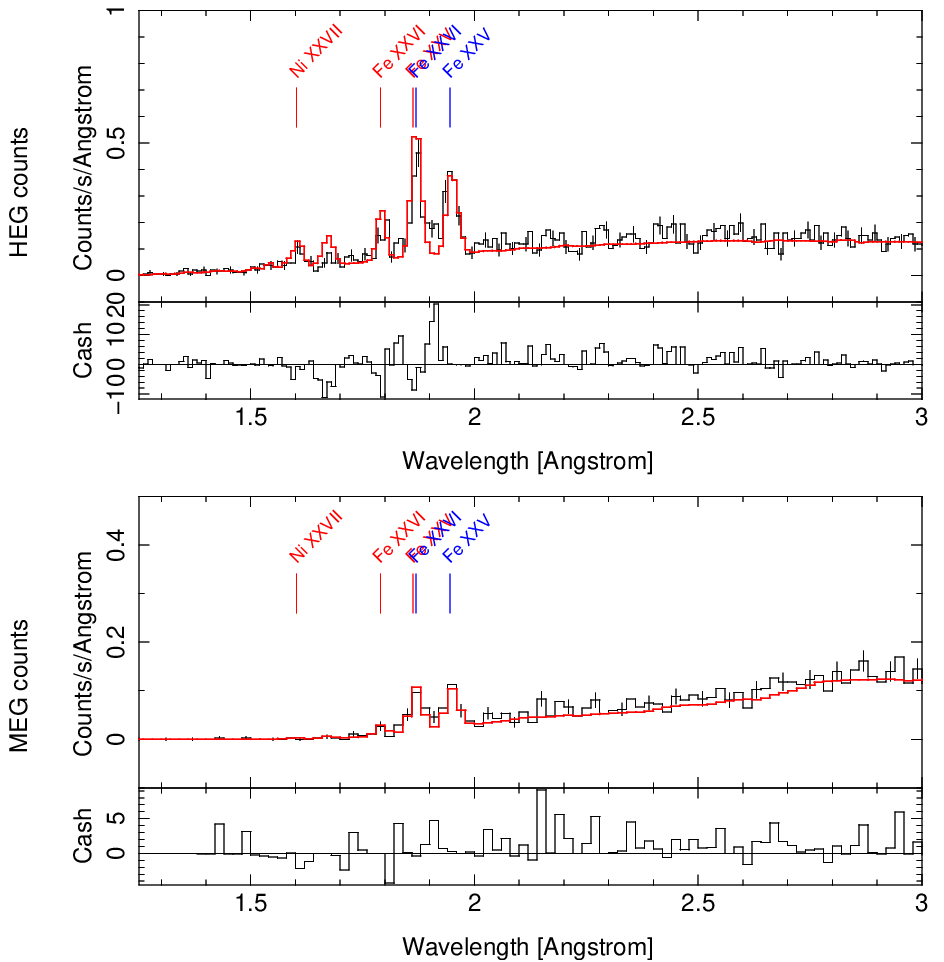
\includegraphics[width = \linewidth]{Chapters/Figures/plasma_short1.png}
    \caption{The 1.25-3.0 \AA\ regions of the HEG (top) and MEG (bottom) spectra of SS 433 observed with the Chandra HETGS on 2018 August 10, compared to a plasma model of the spectra of the blue and red jets. Black line: observed spectrum. Red line: four temperature plasma model providing a generally adequate fit to the spectrum. Line identifications are labeled where there are features in the spectrum and confirmed by the model. The red characters label the emission lines from the Western jet while the blue ones from the Eastern jet. The Cash statistic residuals are shown at the bottom of each spectrum. Fe {\sc xxvi} from the Eastern jet and Fe {\sc xxv} from the Western jet are blended. }    \label{plasma_short1}
\end{figure}


\begin{figure}
    \centering
    \includegraphics[width = \linewidth]{Chapters/Figures/plasma_short2.png}
    \caption{Same as Figure~\ref{plasma_short1}, except for the 2.8-7.5 \AA\ region. Si {\sc xiv} and Si {\sc xiii} are well fit.}
    \label{plasma_short2}
\end{figure}

\begin{figure}
    \centering
    \includegraphics[width = \linewidth]{Chapters/Figures/plasma_short3.png}
    \caption{Same as Figure~\ref{plasma_short2}, except for the 7-11 \AA\ region. }
    \label{plasma_short3}
\end{figure}


\newpage
\section{The 96 ksec Observation}

Using the similar fitting routine as the short observation, the four-temperature plasma model fit the whole long observation. The interstellar medium (ISM) absorption $N_H = (1.23 \pm 0.0024) \times 10^{22}$ $\mathrm{cm^{-2}}$.\par 


Figure~\ref{long_plasma1} - \ref{long_plasma3} shows that highly ionized iron lines from the Eastern jet were occulted during the eclipse and silicon lines from the receding (Eastern) jet also appeared fainter. This suggests that both the hot and cool part of the Eastern jet were likely occulted by the companion star. Given that ions which exist in different temperatures has a similar width and redshift, we assume that the flow has a constant jet velocity and opening angle. 
Table~\ref{tab:plasma_long} shows the results of the four-temperature plasma model for the long observation. Comparing with the plasma model results for the short observation, it is noticeable that the metal abundance (Fe, S, Si, Mg) decreased by 9.6\% and Ni abundance decreased by 29\%. The emission measures of the Eastern jet in the $126 \times 10^6$ K temperature region decreased significantly by 74\% before and during the eclipse. This matches with the spectrum, showing the disappearance of Fe {\sc xxvi} and faint lines from the Eastern jet due to the eclipse. 









\begin{figure}
    \centering
    \includegraphics[width = \linewidth]{Chapters/Figures/long_plasma_whole1.png}
    \caption{The 1.25-3.0 portions of the HEG and MEG spectra of SS 433 observed with the Chandra HETGS during 2018 August 13 - 14, compared to a model of the spectra of the blue and red jets. Red line: four temperature plasma model providing a generally adequate fit to the spectrum. Line identifications are labeled where there are features in the spectrum and confirmed by the model. The red characters label the emission lines from the Western jet while the blue ones from the Eastern jet. The Cash statistic residuals are shown at the bottom of each spectrum. Fe {\sc xxvi} from the Eastern jet and Fe {\sc xxv} from the Western jet are blended.}
    \label{long_plasma1}
\end{figure}

\begin{figure}
    \centering
    \includegraphics[width = \linewidth]{Chapters/Figures/long_plasma_whole2.png}
    \caption{Same as Figure~\ref{long_plasma1}, except for the 2.8 - 7.5 \AA\ region. }
    \label{long_plasma2}
\end{figure}


\begin{figure}
    \centering
    \includegraphics[width = \linewidth]{Chapters/Figures/long_plasma_whole3.png}
    \caption{Same as Figure~\ref{long_plasma1}, except for the 7-11 \AA region. }
    \label{long_plasma3}
\end{figure}













\begin{deluxetable}{rcccccc}
\tablecolumns{5}
\tablewidth{0pc}
\tabletypesize{\small}
\tablecaption{Jet Parameters from a Multitemperature model for the 100 ksec observation
\label{tab:plasma_long} }
\tablehead{& & & & &Western jet & Eastern jet\\
\colhead{T} &  \colhead{$n_e$} &  \colhead{vturb} & \colhead{metal} & \colhead{Ni} & \colhead{EM} & \colhead{EM} \\
  \colhead{($\times 10^6$ K)}  & \colhead{($\times 10^{14} \mathrnm{cm^{-3}}$)}& \colhead{(km/s)} &\colhead{($\odot$ metal)} & \colhead{($\odot$ Ni)} & \colhead{($\times 10^{57}\mathrm{cm^{-3}}$)} & \colhead{($\times 10^{57}\mathrm{cm^{-3}}$)}}
\startdata
6.3& 1 & 1662.2 & 2.79 & 30.21 & 0.58 &  0.23 \\
12.6& 1 & 1662.2& 2.79 & 30.21 & 2.09 &  $<$0.037 \\ 
31.6& 1 & 1662.2& 2.79 & 30.21 & 2.96 &  $<$0.037 \\
126.& 1 & 1662.2& 2.79 & 30.21 & 15.87 &  3.67 \\
\enddata
\end{deluxetable}






  \chapter{Discussion}

\section{Discrepancies in the Observed Redshifts of the Jets}
The redshifts of both jets in the short observation almost match to the predicted values - the redshift for the Eastern jet is slightly out of the error bar of predicted value (See the left part of Figure~\ref{redshift}).
Within the long observation, no significant redshifts change were observed for either jet. For the long observation, the predicted redshift value of the Western jet was -0.0097 and the predicted redshift value of the Eastern jet was 0.087. However, the average observed redshift values for the Western jet was 0.034, about 450\% larger than the predicted value. The difference being $\Delta z = 0.0437$ or 13110 km $\mathrm{s^{-1}}$. Since the discrepancy was already present at the beginning of the long observation, it is unclear when and how the redshift changed abnormally. Figure~\ref{redshift} shows the discrepancy between the observed and the predicted redshifts. The match between the predicted redshift and observed redshift of the Eastern jet indicate that two jets' behaviours were likely independent in the X-ray emitting region. This match to the conclusion drawn in \cite{Marshall2013}. According to Equation~\ref{relativistic_doppler}, the observed redshift depends on both the angle that the jet makes to the line of sight $\theta$, and on the velocity of the jet $v$. Therefore, the observed discrepancy indicates that the X-ray jet's velocities may have been affected by the environment which also perturbed the direction of the jet. 

According to Equation~\ref{relativistic_doppler}, if the redshift is 0.034, in order to make Western jet's speed to be 0.26c, $\theta$ needs to be 90.34\degree. If the redshift is -0.0097 as predicted, $\theta$ needs to be 99.69\degree. In order to have the jet have $\theta$ be the predicted value 99.69 \degree, the velocity needs to be 0.45c, which is almost twice of the accepted value, 0.26c. Figure~\ref{thetav} shows the relationship between $\theta$ and $v$, indicating that velocity perturbations alone are insufficient to explain the large Doppler shift change. Angular deviations of order 9\degree along the direction of precession would be needed to explain the discrepancy.

\begin{figure}
    \centering
    \includegraphics[width = \linewidth]{Chapters/Figures/redshiftv6.png}
    \caption{The observed redshifts from the 2018 observations with Chandra HETG and the predicted redshift according to the kinematic model. The blue and pink bands around the predicted redshift indicates the nutation motion of the jet.}
    \label{redshift}
\end{figure}


\begin{figure}[h!]
    \centering
    \includegraphics[width = \linewidth]{Chapters/Figures/thetav2.png}
    \caption{The relationship between $\theta$ and the velocity of the jet $v$ when the redshift value is 0.034 and -0.0097, respectively, from the 2018 observation. $\theta$ and $v$ }
    \label{thetav}
\end{figure}





\section{Line widths and Positions}
Table~\ref{tab:shortlinefluxes_west} - \ref{tab:longlinefluxes_east} show that the Doppler shifts of the lines in the Western and Eastern jet system are consistent with a single velocity to within the uncertainties for both the short and the long observation. The few deviations are mostly due to blended lines (e.g., line triplets) in each jet, and are not likely indicative of intrinsic variations. The lines responsible for largest deviations are mostly weak or blended, such as lines in the Eastern jet and the Si triplets. The line widths of the emission lines give information about Doppler broadening. Doppler broadening is the broadening of spectral lines due to the Doppler effect. The effect is caused by a distribution of velocities of atoms or molecules. Different velocities of the emitting particles contribute to different Doppler shifts. In plasma physics, the thermal Doppler broadening is one of the explanations to the broadening of a line. Thermal broadening is due to the thermal motion of the particles. The broadening depends only on the frequency of the spectral line, the mass of the emitting particles, and their temperature. Therefore, the broadening can be used for inferring the temperature of an emitting body. The velocity width of an emission line, or the mean speed of a particle can be found by 
\begin{equation}
    v = \dfrac{\sigma c}{\lambda_{obs}},
\end{equation}

where $\sigma$ is the width of the Gaussian. Line width measurements of the short observation for Western and Eastern jets are given in Table~\ref{linewidthshort_west} - \ref{linewidthshort_east}. Systematic errors due to poor continuum modeling, unresolved multiple blend lines modeled as single Gaussians, and unmodeled weak lines are estimated to be of order 100 - 150 km $\mathrm{s^{-1}}$ \citep{Marshall2013}. Although the statistic errors are not included, the line widths are measured in the wavelength 1.5 - 3.5 \AA\ are somewhat smaller than these found in previous papers \citep{Marshall2002, Lopez2006, Marshall2013}. The similarity of the line widths of all wavelengths range indicates that Fe {\sc xxv} is not significantly broader than other lines in the spectrum during the short observation.

\begin{deluxetable}{rc}
\tablecolumns{5}
\tablewidth{0pc}
\tabletypesize{\small}
\tablecaption{Western Jet Line Widths During the Short Observation
\label{linewidthshort_west} }
\tablehead{\colhead{Wavelength Range} &  \colhead{$v$}\\
  \colhead{(\AA)}  & \colhead{(km $\mathrm{s^{-1}}$)}& }
\startdata
1.5-3.5& 1028.2 \\
3.5-6.5& 1031.9 \\ 
6.5-10& 1036.3\\
\enddata
\end{deluxetable}


\begin{deluxetable}{rc}
\tablecolumns{5}
\tablewidth{0pc}
\tabletypesize{\small}
\tablecaption{Eastern Jet Line Widths
\label{linewidthshort_east} }
\tablehead{\colhead{Wavelength Range} &  \colhead{$v$}\\
  \colhead{(\AA)}  & \colhead{(km $\mathrm{s^{-1}}$)}& }
\startdata
1.5-3.5& 1347.6 \\
3.5-6.5& 1342.9 \\ 
6.5-10& 1340.7\\
\enddata
\end{deluxetable}



Since Eastern jet was faint during the long observation, line width measurements of only the long observation for Western jet are shown in Table~\ref{linewidthlong_west}. Line widths for different parts of the long observation were found separately. Comparing with the high-energy lines of the western jet in the short observation  (1028 km $\mathrm{s^{-1}}$, line widths of the western jet are significantly wider in the long observation (an average of 2146 km $\mathrm{s^{-1}}$). Within the long observation, lines in 1.5 - 3.5 \AA\ range are significantly broader than the lines in other ranges. Although Fe {\sc xxv} from the Western jet consists of unresolved lines, Fe {\sc xxvi} and Ni {\sc xxvii} (2100 km $\mathrm{s^{-1}}$) also dominate the broad line measurements in 1.5 - 3.5 \AA\ range. Ni is highly overabundant, as found in the plasma fitting in Chapter 4 (42.61 $\odot$ Ni for short observation and 30.21 $\odot$ Ni for the long observation). The line measurements in 6.5 - 10 \AA\ are somewhat larger than those reported in previous papers (729 $\pm$ 34 km $\mathrm{s^{-1}}$ \citep{Marshall2013}). More accurate values could be derived if more lines are fitted in longer wavelength range. 


\begin{deluxetable}{rccccc}
\tablecolumns{5}
\tablewidth{0pc}
\tabletypesize{\small}
\tablecaption{Western Jet Line Widths During the Long Observation
\label{linewidthlong_west} }
\tablehead{\colhead{} &  \colhead{Part \sc i}&  \colhead{Part \sc ii}&  \colhead{Part \sc iii}&  \colhead{Part \sc iv}&  \colhead{Part \sc v}\\ \colhead{Wavelength Range} &  \colhead{$v$}&  \colhead{$v$}&  \colhead{$v$}&  \colhead{$v$}&  \colhead{$v$}\\
  \colhead{(\AA)}  & \colhead{(km $\mathrm{s^{-1}}$)} & \colhead{(km $\mathrm{s^{-1}}$)}& \colhead{(km $\mathrm{s^{-1}}$)}& \colhead{(km $\mathrm{s^{-1}}$)}& \colhead{(km $\mathrm{s^{-1}}$)} }
\startdata
1.5 - 3.5&	15.7&	2245.3&	2213.3&	2042.2&	2232.4\\
3.5 - 6.5&	1064.1&	1082.8&	804.8&	984.2&	1293.9\\
6.5 - 10&	1120.8&	1136.2&	843.5&	1029.3&	1352.9\\

\enddata
\end{deluxetable}



\section{Jet Emission Line Fluxes}
Figure~\ref{west_flux} - \ref{east_flux} shows the line flux changes in the Western and Eastern jets, respectively. All the lines from the Western jet, including iron lines in the hardest energy region, appear on the spectrum with considerable line fluxes. The flux of Fe {\sc xxv} and Fe {\sc xxvi} from the Western jet did not decrease during the eclipse. Instead, these lines were significantly brighter than they were during the short observation 3 days ago. The changes of the fluxes of Fe {\sc xxv} and Fe {\sc xxvi} during the long observation did not show a regularly increasing or decreasing trend, indicating the fluctuations might be due to environmental activities instead of the eclipse. The increasing flux of and Si suggests that the cooler region of the Western jet was not occulted by the donor. This does not align with the model shown in Fig~\ref{geomtry_ss433} developed by \citep{Lopez2006}, where the outer region of the Western jet was blocked by the donor during the eclipse.\par 
In the Eastern jet, the flux of Fe {\sc xxv} goes to zero during the whole long observation. This suggests that the hard energy region of the Eastern jet was blocked by the donor. The blended lines of Fe {\sc xv} west and Fe {\sc xxvi} east made it harder to say whether the other Fe {\sc xxvi} from the Eastern jet was also blocked or not. Voigt profile modelling was able distinguish the two lines and fit two Gaussians in one region within a reasonable uncertainty. The flux of Fe {\sc xxvi} was not zero over the whole long observation. This questions the previous suggestion that the hard energy region of the jet was blocked since the temperature of the parts of the jet provide Fe {\sc xxvi} and Fe {\sc xxv} should not have a large difference, which means the region that emits Fe {\sc xxvi} and Fe {\sc xxv} should not be far part away. However, we have not yet been able to quantify this. Also, this observation does not agree with the conclusion by \citep{Marshall2013} that at most 20\% of the jet that provides the blue jet's Fe {\sc xxv} is blocked. The faintness of both hot and cool portions of the Eastern X-ray-emitting jet is unexpected because Eastern jet is usually the one that less blocked by the donor (see Figure~\ref{geomtry_ss433}).

\begin{figure}
    \centering
    \includegraphics[width = \linewidth]{Chapters/Figures/west_flux.png}
    \caption{Flux changes of ten most prominent emission lines of the Western jet over the short and the long observation. The left most point is the line flux of certain element from the short observation while the four right most points are from the long observation. }
    \label{west_flux}
\end{figure}




\begin{figure}
    \centering
    \includegraphics[width = \linewidth]{Chapters/Figures/east_flux.png}
    \caption{Same as Fig~\ref{west_flux}, but for the Eastern jet. The fluxes of Fe{\sc xxv} from the Eastern jet are zero over the long observation. S {\sc xv}, S {\sc xvi} and Si {\sc xiv} are faint and thus have larger uncertainties. Fe {\sc xxvi} east is blended with Fe {\sc xxv} west but with Voigt profile, it is able to fit two gaussians on one region moderately well.}
    \label{east_flux}
\end{figure}


\section{Power Law and Photon Index}

The predicted orbital phase of the end of the observation is 0.109. To verify whether the accretor came out of the eclipse at the end of our observation, we want to find the change of the normalization and the photon index of the spectra over the short and the long observation. Photon index is a measure of the dependence of radiative flux density on energy (or frequency). Normalization $K$ and photon index $\alpha$ satisfy the equation 
\begin{equation}
     N(E) = KE^{-\alpha}.
     \label{powerlaweq}
\end{equation}
After we take the log of Equation~\ref{powerlaweq}, we get 
\begin{equation}
     \mathrm{log}(N(E)) = \mathrm{log}(K) - \alpha \mathrm{log}(E).
     \label{powerlaweq}
\end{equation}
Figure~\ref{powerlaw} shows flux following a power law in energy. The cases when accretor is in the eclipse and out of the eclipse are shown in solid and dash lines.
\begin{figure}
    \centering
    \includegraphics[scale = 0.4]{Chapters/Figures/powerlaw_v2.png}
    \caption{The log plot of power law that explains the relationship between the flux density and the energy. The solid line and the dash line show ideal scenarios when the accretor is in and out of the eclipse. The photon index decrease in this process. This is because the harder energy of the spectrum is more affected by the eclipse and thus when the source is coming out of the eclipse, the flux of the harder energy part will increase.}
    \label{powerlaw}
\end{figure}
Figure~\ref{power_law} show the change of normalization and photon index over time. There is a big jump in the normalizations and photon indices between the short observation and the first part of the long observation.  This might indicate some environmental activities in the low energy part of the jet before and during the long observation. The decreasing trend of photon index indicate that the high energy part of the jet is gradually coming out of the eclipse. Since the value of photon index at the end of the long observation is still 0.23 apart from the one at the short observation, it suggests that the accretor may not have totally come out of the eclipse, which can explain the disappearance of Fe {\sc xxv} of the Eastern jet at the end of the long observation. The reason for the decrease in normalization is uncertain. It is possible that the intrinsic accretion flow was changing during this time. 

\begin{figure}
    \centering
    \includegraphics[width = \linewidth] {Chapters/Figures/powerlaw.png}
    \caption{The power law and photon index of the spectra over the short and the long observation}
    \label{power_law}
\end{figure}



  \chapter{Conclusion}
Although SS 433 have been studied for almost 40 years, it still remains a mysterious astrophysical source.
We observed SS 433 with Chandra, an advance X-ray telescope to explore this enigmatic source. Using the High Energy Transmission Grating System, we took a total of 116 ksec observation, which contains a 20 ksec short observation and a 96 ksec long observation at a new combination of orbital and jet precession phases. This special strategy enables us to map out the spatial variation of the jet's properties, such as temperature and ionization states along the jet. Through fitting two phenomenological models to the spectrum, we were able to probe the changes of the properties of emission lines from both jets between the two observations and within the long observation. The plasma model enables us the probe the physical conditions in the jet base.\par 

The unexpected redshift observed in the Western jet reinforce the hypothesis of the previous paper that the Eastern and Western jets were moving independent to each other. The varying normalization may suggest a changing intrinsic accretion flow during the observation. The unexpected line flux of the Western jet during the eclipse and the photon index of the power law also give some insights to the size of the donor star, which could be further studied in the future. \par 
This work gives rise to numerous questions that could be addressed in future studies of SS 433, both observational as well as theoretical. Plasma models for different parts in the long observation could be fit and compared so that we can probe physical condition changes of the jet during the eclipse more carefully. Better plasma models could also be developed to fit the natural properties of the jet more accurately. Therefore, this is not the end of this research project. We plan to continue researching on this observation of SS 433 to refine our approach to analyze this subject and get a better understanding to it.
  \chapter*{Appendix}

\begin{figure}[t]
    \centering
        \includegraphics[width = \linewidth]{Chapters/Figures/long_pheno0_heg.png}
        \caption{The X-ray spectrum of SS 433 observed with the Chandra HETGS on 2018-08-13, when the accretor's orbit phase is 0.022. This set of figures show the spectrum formed from the HEG data of the first 19.2 ksec of the long observation. The disappearance of Fe {\sc xxv} indicates that the region of the Eastern jet showing Fe {\sc xxv} is blocked.}
    \label{long_pheno0_heg}
\end{figure}


\begin{figure}[t]
    \centering
        \includegraphics[width = \linewidth]{Chapters/Figures/long_pheno0_meg.png}
        \caption{Same as Figure~\ref{long_pheno0_heg}, but showing the MEG spectrum.}
    \label{long_pheno0_meg}
\end{figure}





\begin{figure}[t]
    \centering
        \includegraphics[width = \linewidth]{Chapters/Figures/long_pheno1_heg.png}
        \caption{Same as Figure~\ref{long_pheno0_heg} but showing the spectrum from the HEG data of the second 19.2 ksec of the long observation. The orbit phase of the accretor is 0.039.}
    \label{long_pheno1_heg}
\end{figure}


\begin{figure}[t]
    \centering
        \includegraphics[width = \linewidth]{Chapters/Figures/long_pheno1_meg.png}
        \caption{Same as Figure~\ref{long_pheno1_heg}, but showing the MEG spectrum.}
    \label{long_pheno1_meg}
\end{figure}


\begin{figure}[t]
    \centering
        \includegraphics[width = \linewidth]{Chapters/Figures/long_pheno2_heg.png}
        \caption{Same as Figure~\ref{long_pheno0_heg} but showing the spectrum formed from the HEG data of the third 19.2 ksec part of the long observation. The orbit phase of the accretor is 0.057.}
    \label{long_pheno2_heg}
\end{figure}


\begin{figure}[t]
    \centering
        \includegraphics[width = \linewidth]{Chapters/Figures/long_pheno2_meg.png}
        \caption{Same as Figure~\ref{long_pheno2_heg}, but showing the MEG spectrum.}
    \label{long_pheno2_meg}
\end{figure}


\begin{figure}[t]
    \centering
        \includegraphics[width = \linewidth]{Chapters/Figures/long_pheno3_heg.png}
        \caption{Same as Figure~\ref{long_pheno0_heg} but showing the spectrum formed from the HEG data of the fourth 19.2 ksec of the long observation. The orbit phase of the accretor is 0.074.}
    \label{long_pheno3_heg}
\end{figure}


\begin{figure}[t]
    \centering
        \includegraphics[width = \linewidth]{Chapters/Figures/long_pheno3_meg.png}
        \caption{Same as Figure~\ref{long_pheno3_heg}, but showing the MEG spectrum.}
    \label{long_pheno3_meg}
\end{figure}



\begin{figure}[t]
    \centering
        \includegraphics[width = \linewidth]{Chapters/Figures/long_pheno4_heg.png}
        \caption{Same as Figure~\ref{long_pheno0_heg} except this set of figures show the spectrum formed from the HEG data of the fifth 19.2 ksec of the long observation. The orbit phase of the accretor is 0.092. It is noticeable that the Fe {\sc xxv} from the Eastern jet did not reappear in the spectra as predicted by the ephemeris.}
    \label{long_pheno4_heg}
\end{figure}


\begin{figure}[t]
    \centering
        \includegraphics[width = \linewidth]{Chapters/Figures/long_pheno4_meg.png}
        \caption{Same as Figure~\ref{long_pheno4_heg}, but showing the MEG spectrum}
    \label{long_pheno4_meg}
\end{figure}
  
  %\include{Chapters/}
  %\include{Chapters/further-problem}



  %%% Post face
  % figure menu
  \clearpage{}\label{chap: list of figure}
  \listoffigures
  
  % bibliography
  \bibliography{bib_file/bibliography}
  %\printbibliography
  % index page
  \clearpage{}\label{chap: index}
  \printindex
  

  
  

\end{document}